\documentclass[nobib,notoc,twoside,symmetric]{tufte-book}
\setcounter{tocdepth}{4}
\setcounter{secnumdepth}{4}

\usepackage{marginfix}
%to fix margins
\usepackage{multicol}
%for two-column.
\usepackage{CJKutf8}
%for mandarin

%\usepackage{scrextend} 
%\changefontsizes[11pt]{12pt}

\renewcommand{\footnotesize}{\small}

\geometry{a4paper,landscape,inner=30mm,top=15mm,bottom=10mm,headsep=\baselineskip,textwidth=170mm,marginparsep=8mm,marginparwidth=80mm,textheight=170mm,headheight=\baselineskip}

%\geometry{showframe}% for debugging purposes -- displays the margins

%\usepackage{stmaryrd}
%\usepackage{fontawesome}

\usepackage{amsmath,amsthm,amssymb,amsfonts}
\theoremstyle{definition}
\newtheorem{theorem}{Theorem}[section]
\newtheorem*{theorem*}{Theorem}
\newtheorem{corollary}[theorem]{Corollary}
\newtheorem{lemma}[theorem]{Lemma} 
\newtheorem{proposition}[theorem]{Proposition}
\newtheorem{conj}[theorem]{Conjecture}
\newtheorem{defn}[theorem]{Definition}
\newtheorem{fact}[theorem]{Fact} 
\newtheorem{example}[theorem]{Example} 
\newtheorem{examples}[theorem]{Examples}
\newtheorem{example*}[theorem]{Example*}
\newtheorem{examples*}[theorem]{Examples*}
\newtheorem{remark}[theorem]{Remark}
\newtheorem{remark*}[theorem]{Remark*}
\newtheorem{question}[theorem]{Question}
\newtheorem{assumption}[theorem]{Assumption}
\newtheorem{conjecture}[theorem]{Conjecture}
\newtheorem{convention}[theorem]{Convention}
\newtheorem{justification}[theorem]{Justification} 
\newtheorem{construction}[theorem]{Construction}
\newtheorem{rem}[theorem]{Reminder}
\newtheorem{intuition}[theorem]{Intuition}
\newtheorem{term}[theorem]{Terminology}
\newtheorem{scholium}[theorem]{Scholium}
\newtheorem{requirement}[theorem]{Requirement}
\newtheorem{notation}[theorem]{Notation}
\newtheorem{refinement}[theorem]{Refinement}
\newtheorem{thesis}[theorem]{Thesis}

%for fonts
\usepackage{newpxtext}
%\usepackage[fracspacing]{newpxmath}
\linespread{1.05}

\usepackage{tikz-cd}
\usepackage{macros/tikzfig}
\usepackage{macros/quiver}
\input{macros/thesis.tikzstyles}

% Set up the images/graphics package
\usepackage{graphicx}
\setkeys{Gin}{width=\linewidth,totalheight=\textheight,keepaspectratio}
\graphicspath{{graphics/}}

\title{String diagrams for text}
\author[V.W.]{Vincent Wang-Ma\'{s}cianica}
\date{\today}

% The following package makes prettier tables.  We're all about the bling!
\usepackage{booktabs}

% The units package provides nice, non-stacked fractions and better spacing
% for units.
\usepackage{units}

% The fancyvrb package lets us customize the formatting of verbatim
% environments.  We use a slightly smaller font.
\usepackage{fancyvrb}
\fvset{fontsize=\normalsize}

% Small sections of multiple columns
\usepackage{multicol}

% Squares
\usepackage{stix}

% Provides paragraphs of dummy text
\usepackage{lipsum}

% These commands are used to pretty-print LaTeX commands
\newcommand{\doccmd}[1]{\texttt{\textbackslash#1}}% command name -- adds backslash automatically
\newcommand{\docopt}[1]{\ensuremath{\langle}\textrm{\textit{#1}}\ensuremath{\rangle}}% optional command argument
\newcommand{\docarg}[1]{\textrm{\textit{#1}}}% (required) command argument
\newenvironment{docspec}{\begin{quote}\noindent}{\end{quote}}% command specification environment
\newcommand{\docenv}[1]{\textsf{#1}}% environment name
\newcommand{\docpkg}[1]{\texttt{#1}}% package name
\newcommand{\doccls}[1]{\texttt{#1}}% document class name
\newcommand{\docclsopt}[1]{\texttt{#1}}% document class option name

\usepackage{bussproofs}

\usepackage{xcolor}
\usepackage{xspace}
\def\bB{\begin{color}{blue}}
\def\bO{\begin{color}{orange}}
\def\bG{\begin{color}{green}}
\def\bM{\begin{color}{magenta}}
\def\e{\end{color}\xspace}

%For chesspieces
\usepackage{skak}

%For Brakets
\usepackage{physics}

\usepackage{xspace} 
%\usepackage{enumerate}
\usepackage{color} 
\def\bR{\begin{color}{red}}
\def\bB{\begin{color}{blue}}
\def\e{\end{color}\xspace}

%\usepackage{tocloft}
%\cftsetindents{section}{0em}{2em}
%\cftsetindents{subsection}{0em}{2em}
%\renewcommand\cfttoctitlefont{\hfill\Large\bfseries}
%\renewcommand\cftaftertoctitle{\hfill\mbox{}}

\begin{document}

\maketitle% this prints the handout title, author, and date

%\begin{fullwidth}
%\begin{multicols}{2}
\tableofcontents\marginnote{(Acknowledgements will go in a margin note here.)}
%\end{multicols}
%\end{fullwidth}

\newpage
\vfill
\begin{myboxB}
\centering
\textbf{Novel contributions:}
\begin{itemize}

\item Section \bR REF \e is a pedestrian introduction to weak $n$-category theory (via \texttt{homotopy.io}, underpinned by the theory of associative $n$-categories) from the perspective of generalising familiar string-rewrite systems to higher dimensions. The chief development of this section is a demonstration that context-free grammars and tree-adjoining grammars may be formalised in the $n$-categorical setting.

\item Section \bR REF \e spells out a generative grammar for text using an $n$-categorical signature as a rewrite system, which additionally provides a unified framework from which the Text Circuit Theorem first proved in \bR CITE \e is recovered.

\item Section \bR REF \e introduces the category \textbf{ContRel} of continuous relations. I detail the relationships (or lack thereof) of \textbf{ContRel} to its cousins \textbf{Top} and \textbf{Rel}. Though \textbf{ContRel} is constructed na\"{i}vely, its definition and an exposition of its expressivity from the monoidal perspective appears to be novel.

\item Section \bR REF \e string-diagrammatically characterises set-indexed collections of disjoint open subsets of spaces in \textbf{ContRel} as \emph{sticky spiders} -- special frobenius algebras that satisfy certain interaction relations with an idempotent. The diagrammatic outcome is that reasoning with such set-indexed collections remains as graphically intuitive as with spiders.

\item Section \bR REF \e -- with the aid of a theorem by Friedman \citep{friedman_fom_2005} -- string-diagrammatically characterises a vocabulary of linguistic topological relations in \textbf{ContRel} such as simple connectedness, touching, insideness, and rigid motion.

\item Section \bR REF \e argues for the centrality of explaining communication as a criterion for formal approaches to syntax, and explores the relationship between productive and parsing grammars as organised by a monoidal cofunctor. A diagrammatic treatment of monoidal cofunctor boxes is introduced for this purpose.

\item \bR REF \e is a standalone introduction to the mathematical setup of Montague's \emph{Universal Grammar}, aimed at modern algebraists. An outcome of this section is the placement of text circuits as a natural mathematical development in the broadly conceived programme of Montague Semantics.

\item Appendix \bR REF \e constructs a subcategory of sticky spiders in \textbf{ContRel} on the unit square that behaves as a model of \textbf{FinRel} equipped with a \emph{Turing object} -- a single object in a category with respect to which all other objects and morphisms between them may be encoded. This is of particular relevance to the linguistic phenomenon of \emph{entification} -- that essentially all grammatical categories of words and even phrases have noun-equivalents, e.g. $\texttt{to run} \simeq \texttt{running}$, $\texttt{Bob drinks} \simeq \texttt{the fact that Bob drinks}$. The presence of a Turing object in a symmetric monoidal category additionally provides a semantic model for higher-order processes of generic input type, and for \emph{lasso diagrams}.

\item In Section \bR REF \e, by parsing text as circuits (Section \bR REF \e) and using monoidal cofunctor boxes (Section \bR REF \e) to interpret those circuits in \textbf{ContRel} as iconic representations equipped with a vocabulary of lingustic-topological concepts (Section \bR REF \e), I compute some metaphors by hand.

\end{itemize}
\end{myboxB}
\vfill
\clearpage
\newpage

\setcounter{chapter}{-1}
\chapter{Context and synopsis}
There are potentially practical and theoretical benefits to a fresh mathematical take on basic linguistics. String diagrams are formal, intuitive, expressive, fun, and pretty. I review the relevant research context.
\newpage
\section{Process Theories}

This section seeks to give an introduction to process theories in an intuitively grounded manner. We aim here to build the process-theoretic mathematics towards linguistic spatial relations -- words like "to the left of" and "between" -- which are a common ground of competence we all possess. Here we only focus on geometric relations in two dimensional Euclidean space equipped with notions of metric and distance. This section provides adequate foundations to follow \citep{}talkspace, in which I demonstrate how text circuits can be obtained from sentences and how such text circuits interpreted in the category of sets and relations \textbf{Rel} provides a semantics for such sentences. Moreover, this section motivates the question of how to express the (arguably more primitive \citep{}piaget) linguistic topological concepts -- such as "touching" and "inside" -- the mathematics of which will be in Chapter \ref{}; the reader may skip straight to that chapter after this section if they are uninterested in syntax. We close this section with a brief aside on how process theories relate to mathematical foundations and computer science.

A \emph{process} is something that transforms some number of input system types to some number of output system types. We depict systems as wires, labelled with their type, and processes as boxes. We read processes from left to right.
\[\tikzfig{proctheory/process}\]
Processes may compose in parallel, which we depict as vertically stacking boxes.
\[\tikzfig{proctheory/processpar}\]
Processes may compose sequentially, which we depict as connecting wires of the same type from left to right.
\[\tikzfig{proctheory/processseq}\]
In these diagrams only input-output connectivity matters: so we may twist wires and slide boxes along wires to obtain different diagrams that still refer to the same process. So the diagram below is equal to the diagram above.
\[\tikzfig{proctheory/processeq}\]
Some processes have no inputs; we call these \emph{states}. 
\[\tikzfig{proctheory/state}\]
Some processes have no outputs; we call these \emph{tests}.
\[\tikzfig{proctheory/test}\]
A process with no inputs and no outputs is a \emph{number}; the number tells us the outcome of applying tests to a composite of states modified by processes.
\[\tikzfig{proctheory/number}\]

A process theory is given by the following data\footnote{Formally, process theories are symmetric monoidal categories []; see section \ref{}.}:
\begin{itemize}
    \item A collection of systems
    \item A collection of processes along with their input and output systems
    \item A methodology to compose systems and processes sequentially and in parallel, and a specification of the unit of parallel composition.
    \item A collection of equations between composite processes
\end{itemize}

\begin{example}[Linear maps with direct sum]
Systems are finite-dimensional vector spaces over $\mathbb{R}$. Processes are linear maps, expressed as matrices with entries in $\mathbb{R}$.\\
Sequential composition is matrix multiplication. Parallel composition of systems is the direct sum of vector spaces $\oplus$. The parallel composition of matrices $\mathbf{A}, \mathbf{B}$ is the block-diagonal matrix
$$\begin{bmatrix}
\mathbf{A} & \mathbf{0} \\
\mathbf{0} & \mathbf{B}
\end{bmatrix}$$
The unit of parallel composition is the singleton 0-dimensional vector space.
States are row vectors. Tests are column vectors. The numbers are $\mathbb{R}$.\footnote{Usually the monoidal product is written with the symbol $\otimes$, which denotes hadamard product for linear maps. The process theory we have just described takes the direct sum $\oplus$ to be the monoidal product. To avoid confusion we will use the linear algebraic notation when linear algebra is concerned.}
\end{example}

\begin{example}[Sets and functions with cartesian product]
Systems are sets $A,B$. Processes are functions between sets $f: A \rightarrow B$. Sequential composition is function composition. Parallel composition of systems is the cartesian product of sets: the set of ordered pairs of two sets.
\[A \otimes B = A \times B := \{(a,b) \ | \ a \in A, b \in B\}\]
The parallel composition $f \otimes g : A \times C \rightarrow B \times D$ of functions $f: A \rightarrow B$ and $g: C \rightarrow D$ is defined:
\[f \otimes g := (a,c) \mapsto (f(a),g(c))\]
The unit of parallel composition is the\footnote{There are many singletons, but this presents no problem for the later formal definition because they are all equivalent up to unique isomorphism.} singleton set $\{\star\}$. States of a set $A$ correspond to elements $a \in A$\footnote{We forgo the usual categorical definition of points from the terminal object in favour of generalised points from the monoidal perspective.}. Every system $A$ has only one test $a \mapsto \star$\footnote{This is since the singleton is terminal in \textbf{Set}.}. There is only one number.
\end{example}

\begin{example}[Sets and relations with cartesian product]
Systems are sets $A,B$. Processes are relations between sets $\Phi \subseteq A \times B$, which we may write in either direction $\Phi^*: A \nrightarrow B$ or $\Phi_*: B \nrightarrow A$.\footnote{Relations between sets are equivalently matrices with entries from the boolean semiring. Relation composition is matrix multiplication with the boolean semiring. $\Phi^*,\Phi_*$ are the transposes of one another.}
Sequential composition is relation composition:
\[A \overset{\Phi}{\nrightarrow} B \overset{\Psi}{\nrightarrow} C := \{(a,c) \ | \  a \in A, \ c \in C, \ \exists b_{\in B}: (a,b) \in \Phi \wedge (b,c) \in \Psi  \}\]
Parallel composition of systems is the cartesian product of sets. The parallel composition of relations $A \otimes C \overset{\Phi \otimes \Psi}{\nrightarrow} B \otimes D$ of relations $A \overset{\Phi}{\nrightarrow} B$ and $C \overset{\Psi}{\nrightarrow} D$ is defined:
\[\Phi \otimes \Psi := \{\big( (a,c) , (b,d) \big) \ | \ (a,b) \in \Phi \wedge (c,d) \in \Psi\}\]
The unit of parallel composition is the singleton. States of a set $A$ are subsets of $A$. Tests of a set $A$ are also subsets of $A$.
\end{example}

\subsection{What does it mean to copy and delete?}

Now we discuss how we might define the properties and behaviour of processes by positing equations between diagrams. Let's begin simply with two intuitive processes \emph{copy} and \emph{delete}:
\[\tikzfig{proctheory/copydelete}\]

\begin{example}[Linear maps]
Consider a vector space $\mathbf{V}$, which we assume includes a choice of basis. The copy map is the rectangular matrix made of two identity matrices:
\[\Delta_\mathbf{V}: \mathbf{V} \rightarrow \mathbf{V} \oplus \mathbf{V} := \begin{bmatrix} \mathbf{1}_\mathbf{V} & \mathbf{1}_\mathbf{V} \end{bmatrix}\]
The delete map is the column vector of 1s:
\[\epsilon_\mathbf{V}: \mathbf{V} \rightarrow \mathbf{0} := \begin{bmatrix} 1 \\ \vdots \\ 1 \end{bmatrix}\]
\end{example}

\begin{example}[Sets and functions]
Consider a set $A$. The copy function is defined:
\[\Delta_A : A \rightarrow A \times A := a \mapsto (a,a)\]
The delete funtion is defined:
\[\epsilon_A : A \rightarrow \{\star\} := a \mapsto \star\]
\end{example}

\begin{example}[Sets and relations]\label{relcopy}
Consider a set $A$. The copy relation is defined:
\[\Delta_A : A \nrightarrow A \times A := \{\big(a , (a,a) \big) \ | \ a \in A\}\]
The delete relation is defined:
\[\epsilon_A : A \nrightarrow \{\star\} := \{(a,\star) \ | \ a \in A\}\]
\end{example}

We may verify that, no matter the concrete interpretation of the diagram in terms of linear maps, functions or relations copy and delete satisfy the equations in the margin:\marginnote[-10cm]{
Formally, the following equations characterise a cocommutative comonoid internal to a monoidal category.
\begin{equation}\label{cocom}
\scalebox{0.75}{\tikzfig{bestiary/basicrelations}}
\end{equation}
}

It is worth pausing here to think about how one might characterise the process of copying in words; it is challenging to do so for such an intuitive process. The diagrammatic equations in the margin, when translated into prose, provide an answer.
\begin{description}
\item[\textbf{Coassociativity}:] says there is no difference between copying copies.
\item[\textbf{Cocommutativity}:] says there is no difference between the outputs of a copy process.
\item[\textbf{Counitality}:] says that if a copy is made and one of the copies is deleted, the remaining copy is the same as the original.
\end{description}

Insofar as we think this is an acceptable characterisation of copying, rather than specify concretely what a copy and delete does for each system $X$ we encounter, we can instead posit that so long as we have processes $\Delta_X: X \otimes X \rightarrow X$ and $\epsilon_X: X \rightarrow I$ that obey all the equational constraints above, $\Delta_X$ and $\epsilon_X$ are as good as a copy and delete.

\marginnote{
\begin{example}[Not all states are copyable]\label{ex:copyablestate}
Call a state \emph{copyable} when it satisfies the following diagrammatic equation:
\[\tikzfig{proctheory/copyable}\]
In the process theory of sets and functions, all states are copyable. Not all states are copyable in the process theories of sets and relations and of linear maps. For example, consider the two element set $\mathbb{B} := \{0,1\}$, and let $\top : \{\star\} \nrightarrow \mathbb{B} := \{(\star,0),(\star,1)\} \simeq \{0,1\}$. Consider the composite of $\top$ with the copy relation:
\[\top;\Delta_{\mathbb{B}} := \{\big(\star,(0,0)\big),\big(\star,(1,1)\big)\} \simeq \{(0,0),(1,1)\}\]
This is a perfectly correlated bipartite state, and it is not equal to $\{0,1\} \times \{0,1\}$, so $\top$ is not copyable.
\end{example}
}
\marginnote{
\begin{remark}\label{ft:determinism}
The copyability of states is a special case of a more general form of interaction with the copy relation:
\[\scalebox{0.75}{\tikzfig{proctheory/copyablefunc}}\]
A cyan map that satisfies this equation is said to be a homomorphism with respect to the commutative comonoid. In the process theory of relations, those relations that satisfy this equation are precisely the functions; in other words, this diagrammatic equation expresses \emph{determinism}.
\end{remark}}

Here is an unexpected consequence. Suppose we insist that \emph{to copy} in principle also implies the ability to copy \emph{anything} -- arbitrary states. From Example \ref{ex:copyablestate} and Remark \ref{ft:determinism}, we know that this demand is incompatible with certain process theories. In particular, this demand would constrain a process theory of sets and relations to a subtheory of sets and functions. The moral here is that process theories are flexible enough to meet ontological needs. A classical computer scientist who works with perfectly copyable data and processes might demand universal copying along with Equations \ref{cocom}, whereas a quantum physicist who wishes to distinguish between copyable classical data and non-copyable quantum data might taxonomise copy and delete as a special case of a more generic quasi-copy and quasi-delete that only satisfies equations \ref{cocom}.\footnote{Quantum physicists \emph{do} do this; see Dodo: []}

\subsection{What is an update?}\label{ss:update}

In the previous section we have seen how we can start with concrete examples of copying in distinct process theories, and obtain a generic characterisation of copying by finding diagrammatic equations copying satisfies in each concrete case. In this section, we show how to go in the opposite direction: we start by positing diagrammatic equations that characterise the operational behaviour of a particular process -- such as \emph{updating} -- and it will turn out that any concrete process that satisfies the equational constraints we set out will \emph{by our own definition} be an update.\\

Perhaps the most familiar setting for an update is a database. In a database, an \bM entry\e often takes the form of pairs of \bB fields\e and \bO values\e. For example, where a database contains information about employees, a typical entry might look like:
\[\texttt{\bM < \bB\textbf{NAME}\e:\bO Jono Doe\e, \bB\textbf{AGE}\e:\bO 69\e, \bB\textbf{JOB}\e:\bO CONTENT CREATOR\e, \bB\textbf{SALARY}\e:\bO\$420\e, ... >\e}\]
There are all kinds of reasons one might wish to update the value of a field: Jono might legally change their name, a year might pass and Jono's age must be incremented, Jono might be promoted or demoted or get a raise and so on. It was the concern of database theorists to formalise and axiomatise the notion of updating the value of a field -- \emph{independently of the specific programming language implementation of a database} -- so that they had reasoning tools to ensure program correctness []. The problem is reducible to axiomatising a \emph{rewrite}: we can think of updating a value as first calculating the new value, then \emph{putting} the new value in place of the old. Since often the new value depends in some way on the old value, we also need a procedure to \emph{get} the current value.\\

That was a flash-prehistory of \emph{bidirectional transformations} []. Following the monoidal generalisation of lenses in [], a rewrite as we have described above is specified by system diagrammatic equations in the margin, each of which we introduce in prose.

\marginnote[-5cm]{
\begin{description}
\item[\textbf{PutPut}:] Putting in one value and then a second is the same as deleting the first value and just putting in the second.
\[\scalebox{0.5}{\tikzfig{proctheory/putputs}}\]
\item[\textbf{GetPut}:] Getting a value from a field and putting it back in is the same as not doing anything.
\[\scalebox{0.5}{\tikzfig{proctheory/getput}}\]
\item[\textbf{PutGet}:] Putting in a value and getting a value from the field is the same as first copying the value, putting in one copy and keeping the second.
\[\scalebox{0.5}{\tikzfig{proctheory/putget}}\]
\item[\textbf{GetGet}:] Getting a value from a field twice is the same as getting the value once and copying it.
\[\scalebox{0.5}{\tikzfig{proctheory/getget}}\]
\end{description}
}

These diagrammatic equations do two things. First, they completely specify what it means to get and put values in a field in an implementation independent manner; it doesn't matter whether database entries are encoded as bitstrings, qubits, slips or paper or anything else, what matters is the interaction of get and put. Second, the diagrammatic equations give us the right to call our processes \emph{get} and \emph{put} in the first place: we define what it means to get and put by outlining the mutual interactions of get, put, copy, and delete. These two points are worth condensing and rephrasing:
\[
\textbf{A \emph{kind of process} is determined by patterns of interaction with other kinds of processes.}
\]

Now we can diagrammatically depict the process of updating Jono's age, by \bB getting\e Jono's \bO age value\e from their \bM entry\e, incrementing it by 1, and \bB putting\e it back in.

\[\tikzfig{proctheory/incrementage}\]

\subsection{Spatial predicates}

The following simple inference is what we will try to capture process-theoretically:

\begin{itemize}
\item \texttt{Oxford is north of London}
\item \texttt{Vincent is in Oxford}
\item \texttt{Rocco is in London}
\end{itemize}

How might it follow that \texttt{Rocco is south of Vincent}?\\

One way we might approach such a problem computationally is to assign a global coordinate system, for instance interpreting `north' and `south' and `is in' using longitude and latitude. Another coordinate system we might use is a locally flat map of England. The fact that either coordinate system would work is a sign that there is a degree of implementation-independence.\\

This coordinate/implementation-independence is true of most spatial language: we specify locations only by relative positions to other landmarks or things in space, rather than by means of a coordinate system. This is necessarily so for the communication of spatial information between agents who may have very different reference frames.\\

So the process-theoretic modelling aim is to specify how relations between entities can be \emph{updated} and \emph{classified} without requiring individual spatial entities to intrinsically possess meaningful or determinate spatial location.\\

So far we have established how to update properties of individual entities. We can build on what we have so far by observing that a relation between two entities can be considered a property of the pair.

\[placeholder\]

Spatial relations obey certain compositional constraints, such as transitivity in the case of `north of':

\[placeholder\]

Or the equivalence between 'north of' and 'south of' up to swapping the order of arguments:

\[\]

There are other general constraints on spatial relations, such as order-independence: the order in which spatial relations are updated does not (at least for perfect reasoners) affect the resultant presentation. This is depicted diagrammatically as commuting gates:

\[placeholder\]

\subsection{Processes, Sets, Computers}

\newthought{\texttt{Objection:} But what are the \emph{things} that the processes operate on?}

This is a common objection from philosophers who want their ontologies tidy. The claim roughly goes that you can't really reason about processes without knowing the underlying objects that participate on those processes, and since set theory is the only way we know how to spell out objects intensionally in this way, we should stick to sets. In simpler terms, if we're drawing only functions as (black)-boxes in our diagrams, how will we know what they do to the elements of the underlying sets?\\

The short answer is that -- perhaps surprisingly -- reasoning process-theoretically is mathematically equivalent to reasoning about sets and elements for all practical purposes; it is as if whatever is going on \emph{out there} is indifferent to whether we describe using a language of only nouns or only verbs.\\

In the case of set theory, let's suppose that instead of encoding functions as sets, we treat functions as primitive, so that we have a process theory where wires are labelled with sets, and functions are process boxes that we draw. The problem we face now is that it is not immediately clear how we would access the elements of any set using only the diagrammatic language. The solution is the observation that the elements $\{x \ | \ X\}$ of a set $X$ are in bijective correspondence with the functions from a singleton into $X$: $\{ f(\star) \mapsto x \ | \ \{\star\} \overset{f}{\rightarrow} X $. In prose, for any element $x$ in a set $X$, we can find a function that behaves as a pointer to that element $\{\star\} \rightarrow X$. So the states we have been drawing, when interpreted in the category of sets and function, are precisely elements of the sets that label their output wires.\\

The full and formal answer will require the reader to see Section \ref{} which spells out the category theory underpinning process theories. The caveat here is that process theories work for all \emph{practical} purposes, so I make no promises about how diagrams work for the kind of set theories that deals with hierarchies of infinities that set theorists do. For other issues concerning for instance the set of all functions between two sets, that requires symmetric monoidal closure, for which there exist string-diagrammatic formalisms \citep{}.

\newthought{\texttt{Objection:} But if they're expressively the same, what's the point?}

The following rebuttal draws on Harold Abelson's introductory lecture to computer science \citep{} (in which string diagrams appear to introduce programs without being explicitly named as such).\\

There is a distinction between declarative and imperative knowledge. Declarative knowledge is \emph{knowing-that}, for example, 6 is the square root of 36, which we might write $6 = \sqrt{36}$. Imperative knowledge is \emph{knowing-how}, for example, to obtain the square root of a positive number, for instance, by Heron's iterative method: to obtain the square root of $Y$, make a guess $X$, and take the average of $X$ and $\frac{Y}{X}$ until your guess is good enough.\\

Computer science concerns imperative knowledge. An obstacle to the study of imperative knowledge is complexity, which computer scientists manage by black-box abstraction -- suppressing irrelevant details, so that for instance once a square root procedure is defined, the reasoner outside the system does not need to know whether the procedure inside is an iterative method by Heron or Newton, only that it works and has certain properties. These black-boxes can be then composed into larger processes and procedures within human cognitive load.\\

Abstraction also yields generality. For example, in the case of addition, it is not only numbers we may care to add, but perhaps vectors, or the waveforms of signals. So there is an abstract notion of addition which we concretely instantiate for different domains that share a common interface; we may decide for example that all binary operations that are commutative monoids are valid candidates for what it means to be an addition operation.\\

In this light, string diagrams are a natural metalanguage for the study of imperative knowledge; string diagrams in fact independently evolved within computer science from flowcharts describing processes. Process theories, which are equations or logical sentences about processes, allow us to reason declaratively about imperative knowledge. Moreover, string diagrams as syntactic objects can be interpreted in various concrete settings, so that the same diagram serves as the common interface for a process like addition, with compliant implementation details for each particular domain spelled out separately.\label{sec:proctheory}
\newpage
\section{Previously, on DisCoCat}\label{sec:previously}

DisCoCat is a research programme in applied mathematical linguistics that is \textbf{Dis}tributional, \textbf{Co}mpositional and \textbf{Cat}egorical. In this section I will recount a selective development of DisCoCat as relevant for this thesis.

\subsection{Lambek's Linguistics}

Jim Lambek was a jovial man who always carried a wad of twenties.  can't do better than Moortgat's history and exposition of typelogical grammar in \bR CITE \e, so I will borrow Moortgat's phrasing and summarise Lambek's role in the story. Typelogical grammar originated in two seminal papers by Lambek in 1958 and 1961 \bR CITE \e, where Lambek sought “to obtain an effective rule (or algorithm) for distinguishing sentences from non-sentences, which works not only for the formal languages of interest to the mathematical logician, but also for natural languages […]”. The method is to assign grammatical categories -- parts of speech such as nouns and verbs -- logical formulae. Whether a sentence is grammatical or not is obtained from deduction using these logical formulae in a Gentzen-style sequent proof.

\begin{figure}[h!]
\centering
\scalebox{1}{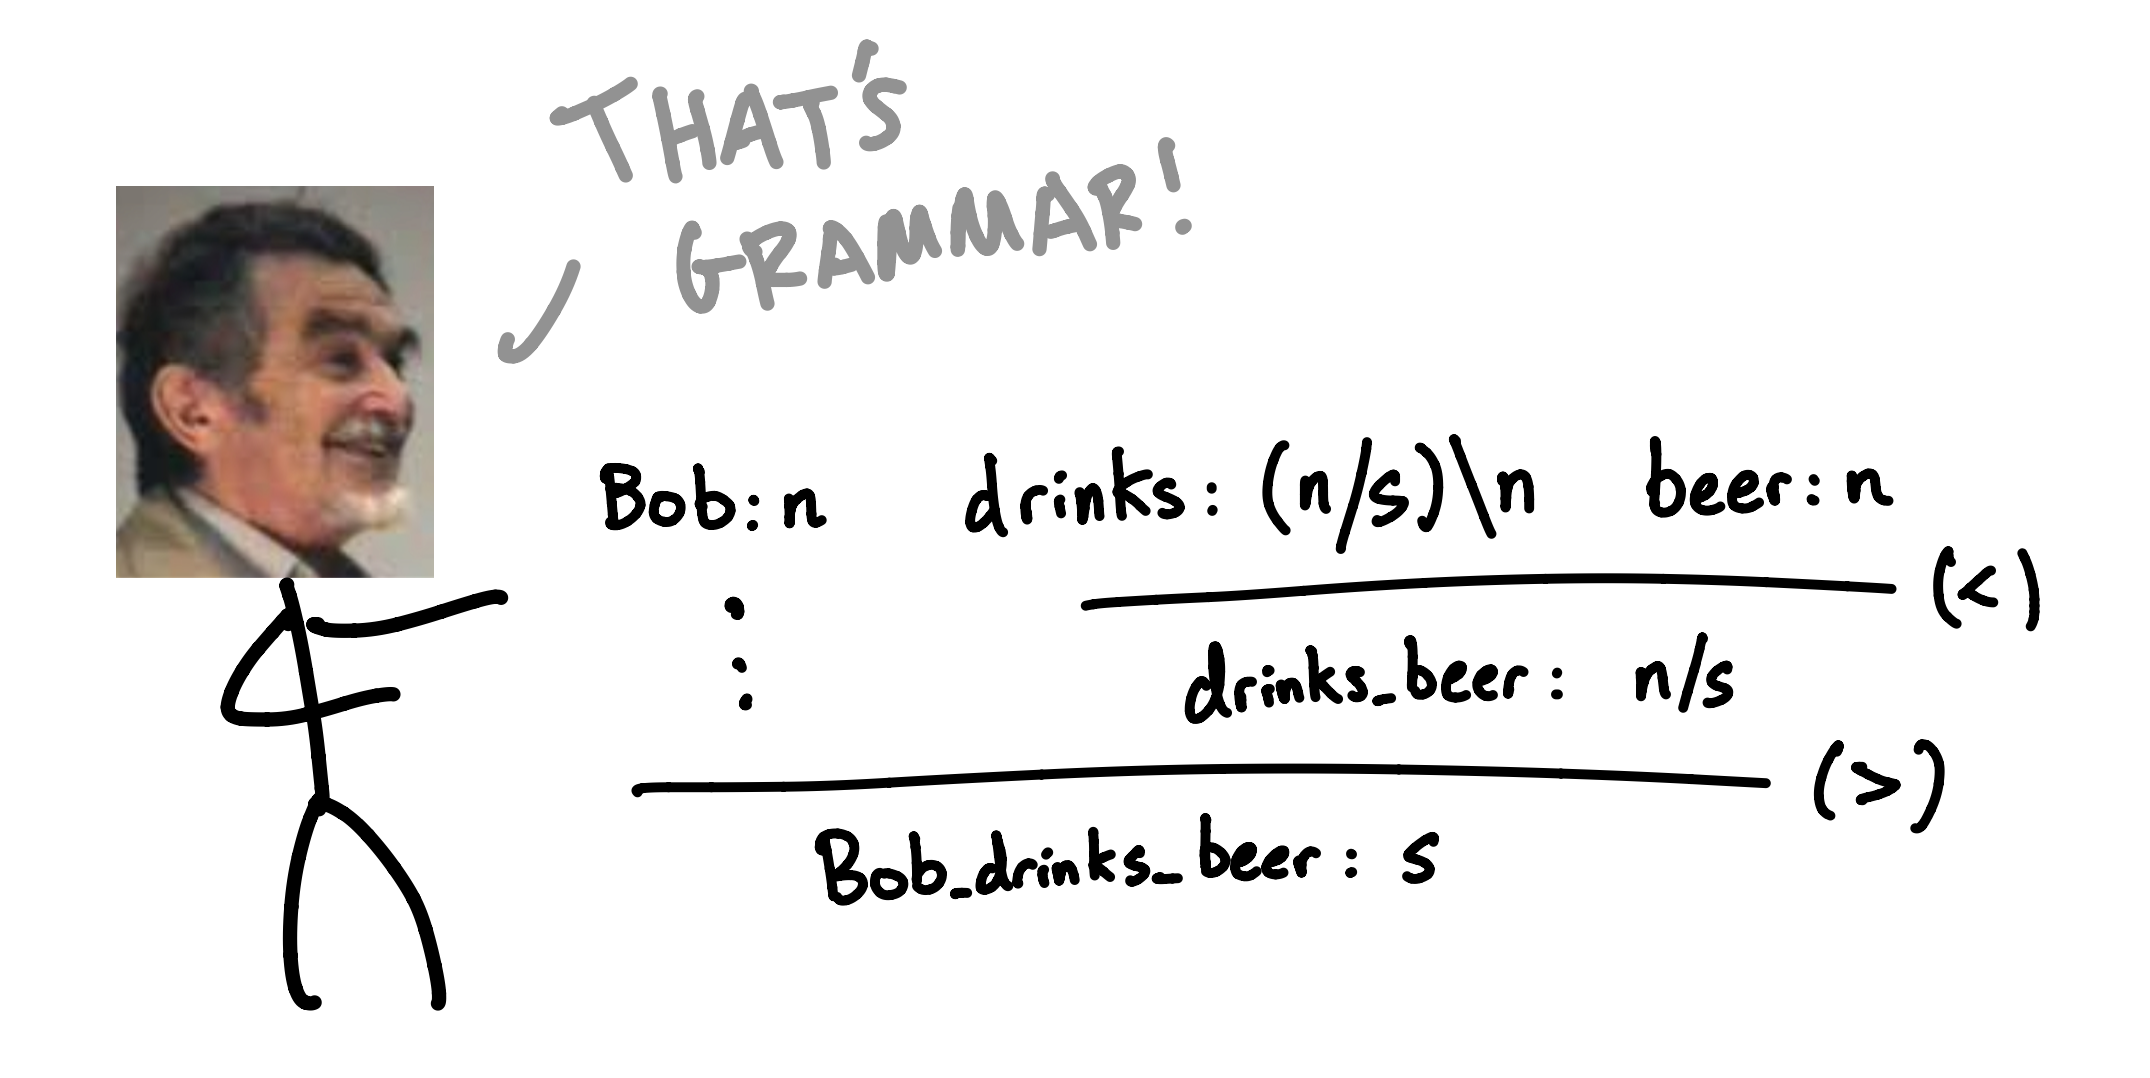
\includegraphics{figures/cartoons/lambek1}}
\caption{In English, we may consider a noun to have type $n$, and a transitive verb $(n/s)\setminus n$, to yield a well-formedness proof of \texttt{Bob drinks beer}. The type formation rules for such a grammar are intuitive. Apart from a stock of basic types $\mathbb{B}$ that contains special final types to indicate sentences, we have two type formation operators $(-/=)$ and $(- \setminus =)$, which along with their elimination rules establish a requirement that grammatical categories require other grammatical categories to their left or right. This is the essence of Lambek's calculi \textbf{NL} and \textbf{L}. CCGs keep the same minimal type-formations, but include extra sequent rules such as type-raising and cross-composition.}
\end{figure}

\begin{figure}[h!]
\centering
\scalebox{1}{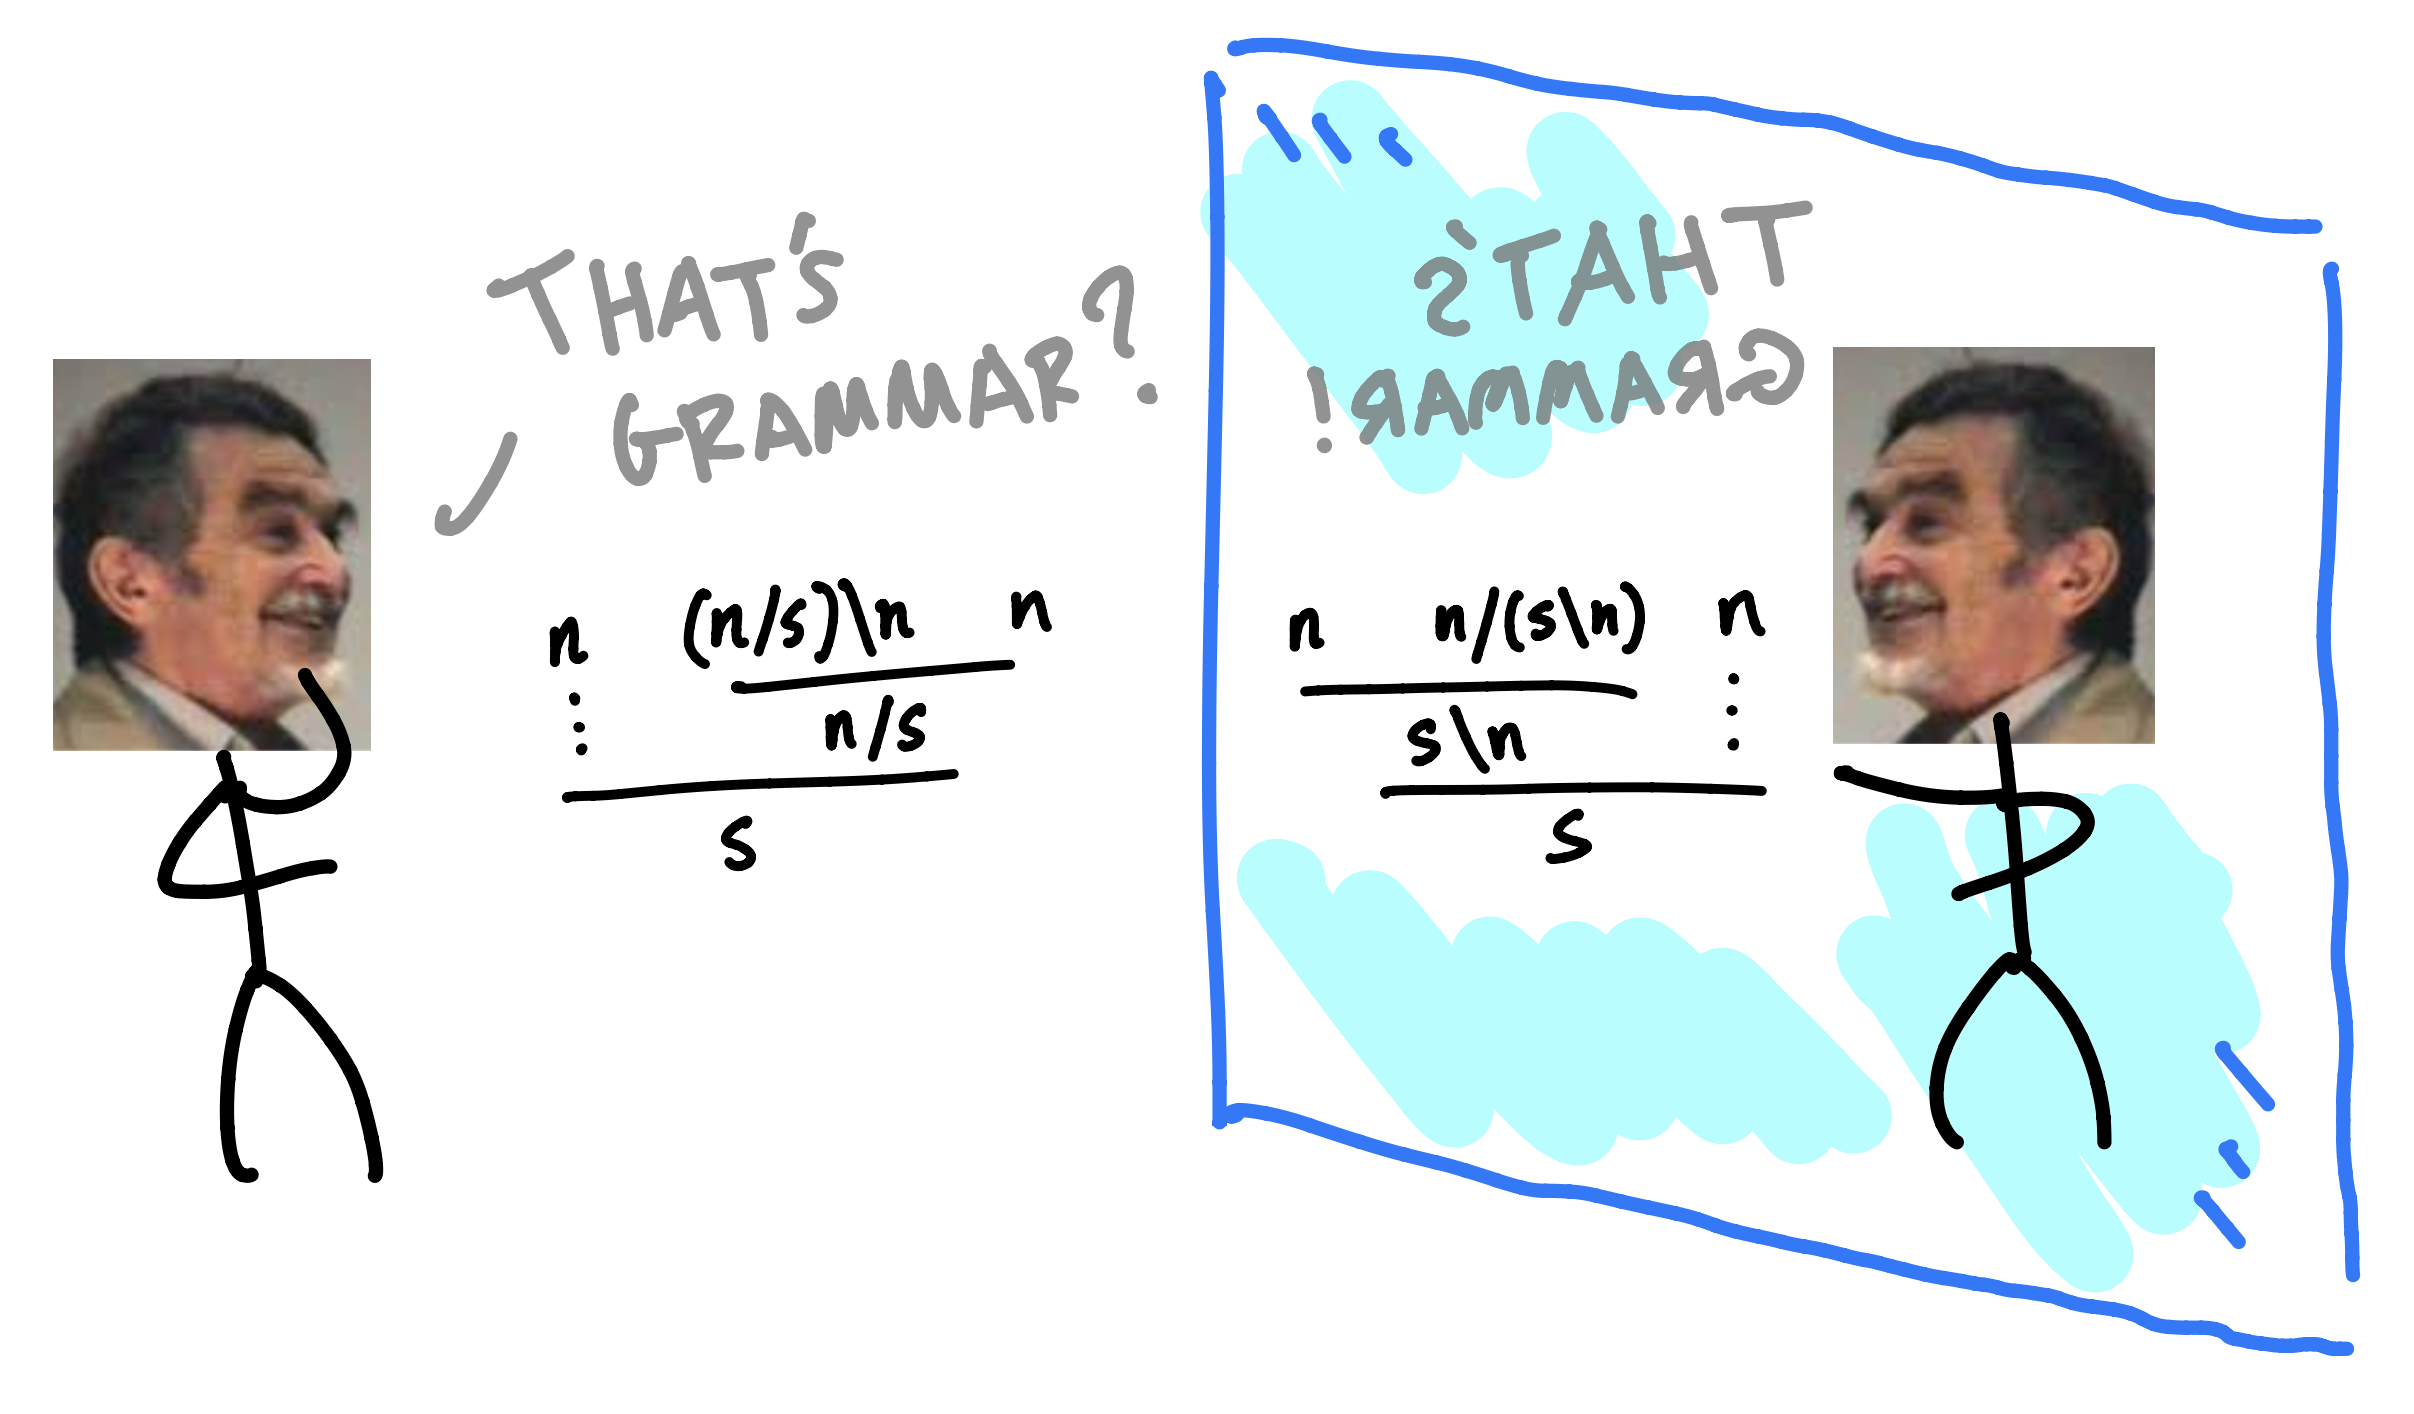
\includegraphics{figures/cartoons/lambek2}}
\caption{We can notice an asymmetry in the above formulation when we examine the transitive verb type $(n/s)\setminus n$ again; it asks first for a noun to the right, and then a noun to the left. We could just as well have asked for the nouns in the other order with the typing $(n/s)\setminus n$ and obtained all of the same proofs.}
\end{figure}

\begin{figure}[h!]
\centering
\scalebox{1}{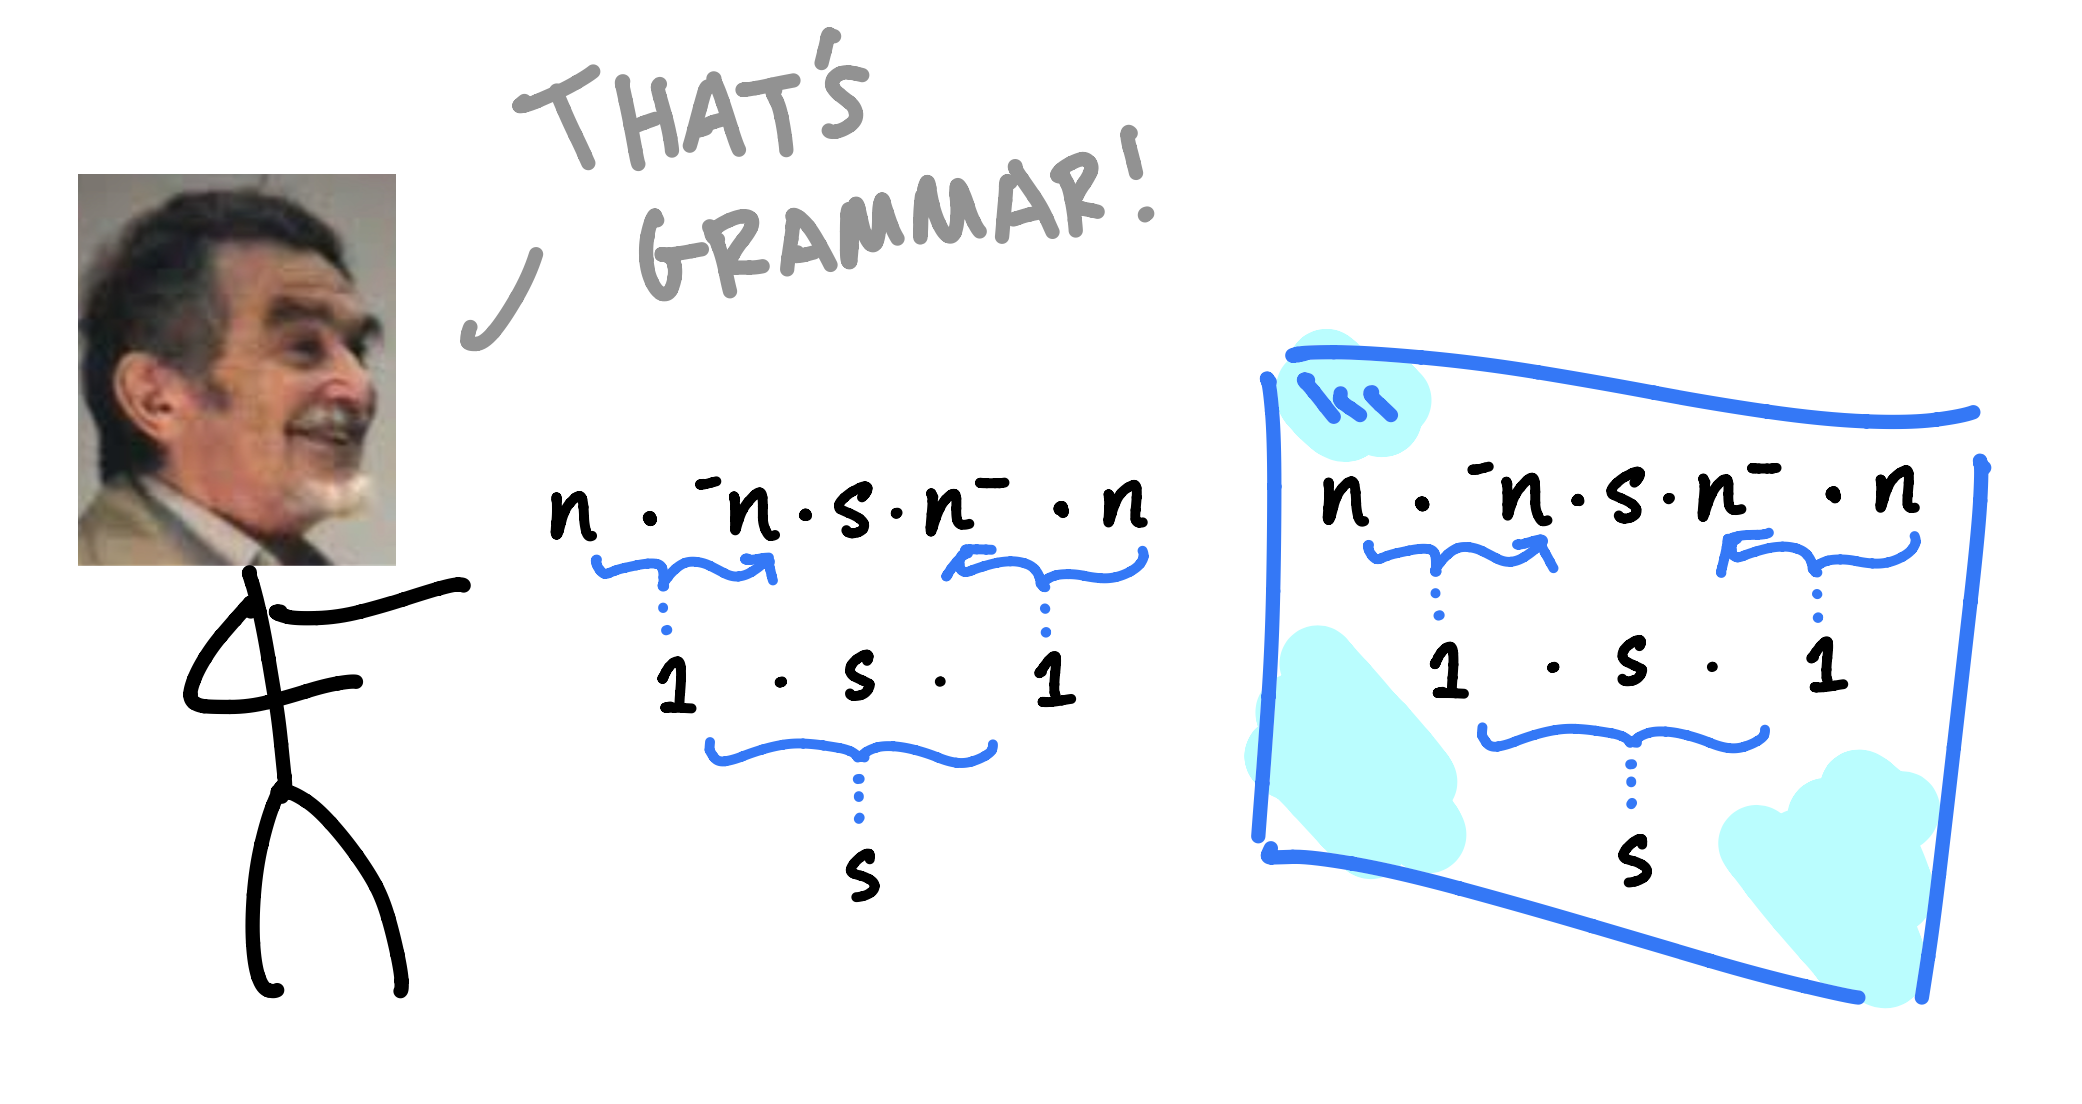
\includegraphics{figures/cartoons/lambek3}}
\caption{To eliminate this asymmetry, Lambek devised pregroup grammars. Whereas a group is a monoid with inverses up to left- and right-multiplication, a pregroup weakens the requirement for inverses so that all elements have distinct left- and right- inverses, denoted $x^{-1}$ and $^{-1}x$ respectively. Eliminating or introducing inverses is a non-identity relation on elements of the pregroup, so we have axioms of the form e.g. $x \cdot ^{-1}x \rightarrow 1 \rightarrow ^{1}x \cdot x$. In this formulation, denoting the multiplication with a dot, both $(n/s)\setminus n$ and $(n/s)\setminus n$ become $^{-1}n \cdot s \cdot n^{-1}$, which just wants a noun to the left and a noun to the right in whatever order to eliminate the flanking inverses to reveal the embedded sentence type. Now we can obtain the same proof of correctness as a series of algebraic reductions.

\begin{align*}
& &n \cdot (^{-1}n \cdot s \cdot n^{-1}) \cdot n\\
&\rightarrow &(n \cdot ^{-1}n) \cdot s \cdot (n^{-1} \cdot n)\\
&\rightarrow & 1 \cdot s \cdot 1\\
&\rightarrow & s
\end{align*}
}
\end{figure}
\clearpage

\subsection{Coecke's Composition}

\begin{figure}[h!]
\centering
\scalebox{0.9}{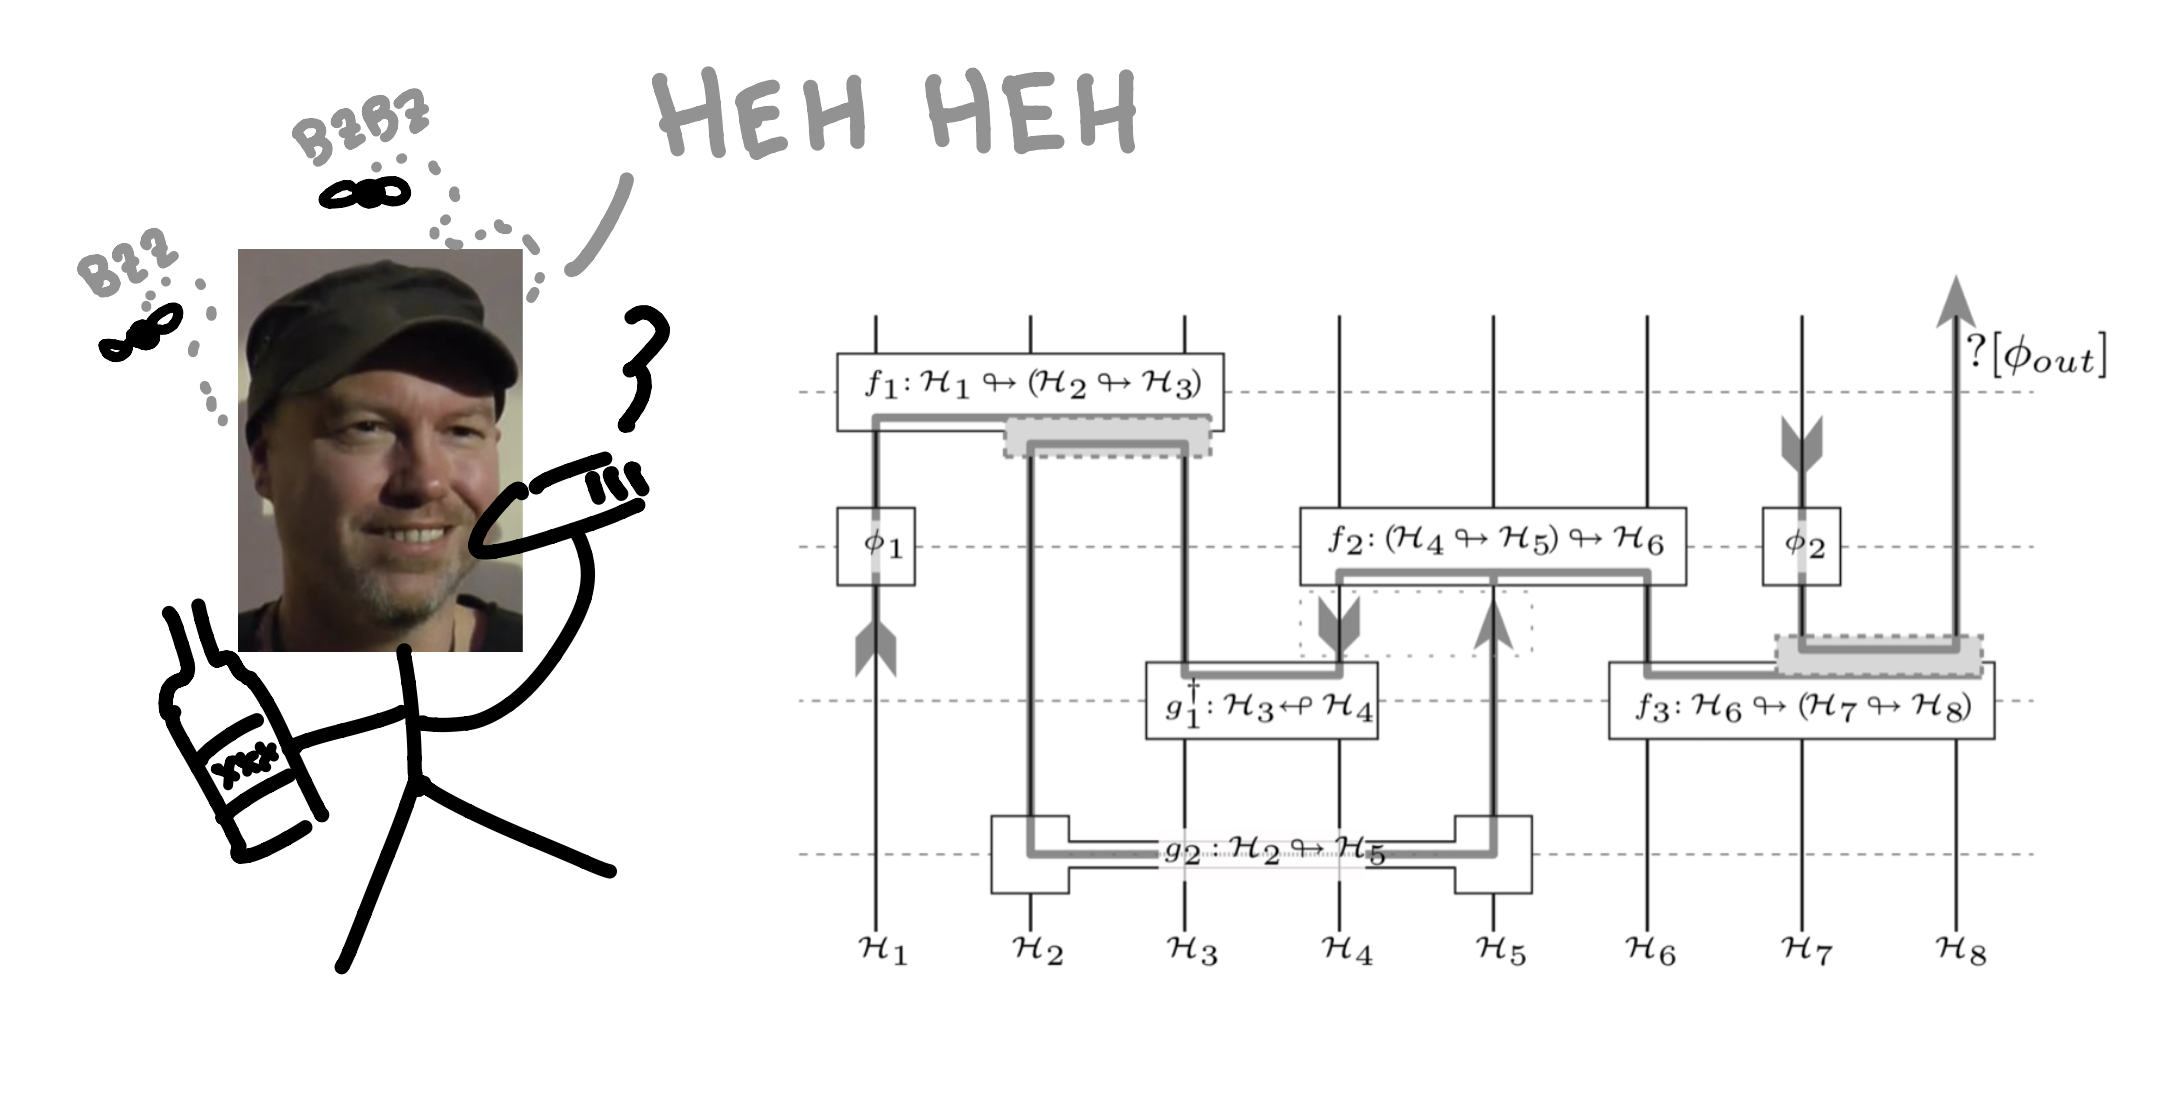
\includegraphics{figures/cartoons/bob1}}
\caption{Meanwhile, an underground grunge vagabond moonlighting as a quantum physicist moonlighting as a computer scientist was causing a shortage of cigars and whiskey in a small English town. He noticed a funny thing about the composition of multiple non-destructive measurements of a quantum system, which was that information could be carried, or flow, between them. So he wrote a paper \bR invitationtoquantum \e, which contained informal diagrams that looked like this.}
\end{figure}

\begin{figure}[h!]
\centering
\scalebox{0.9}{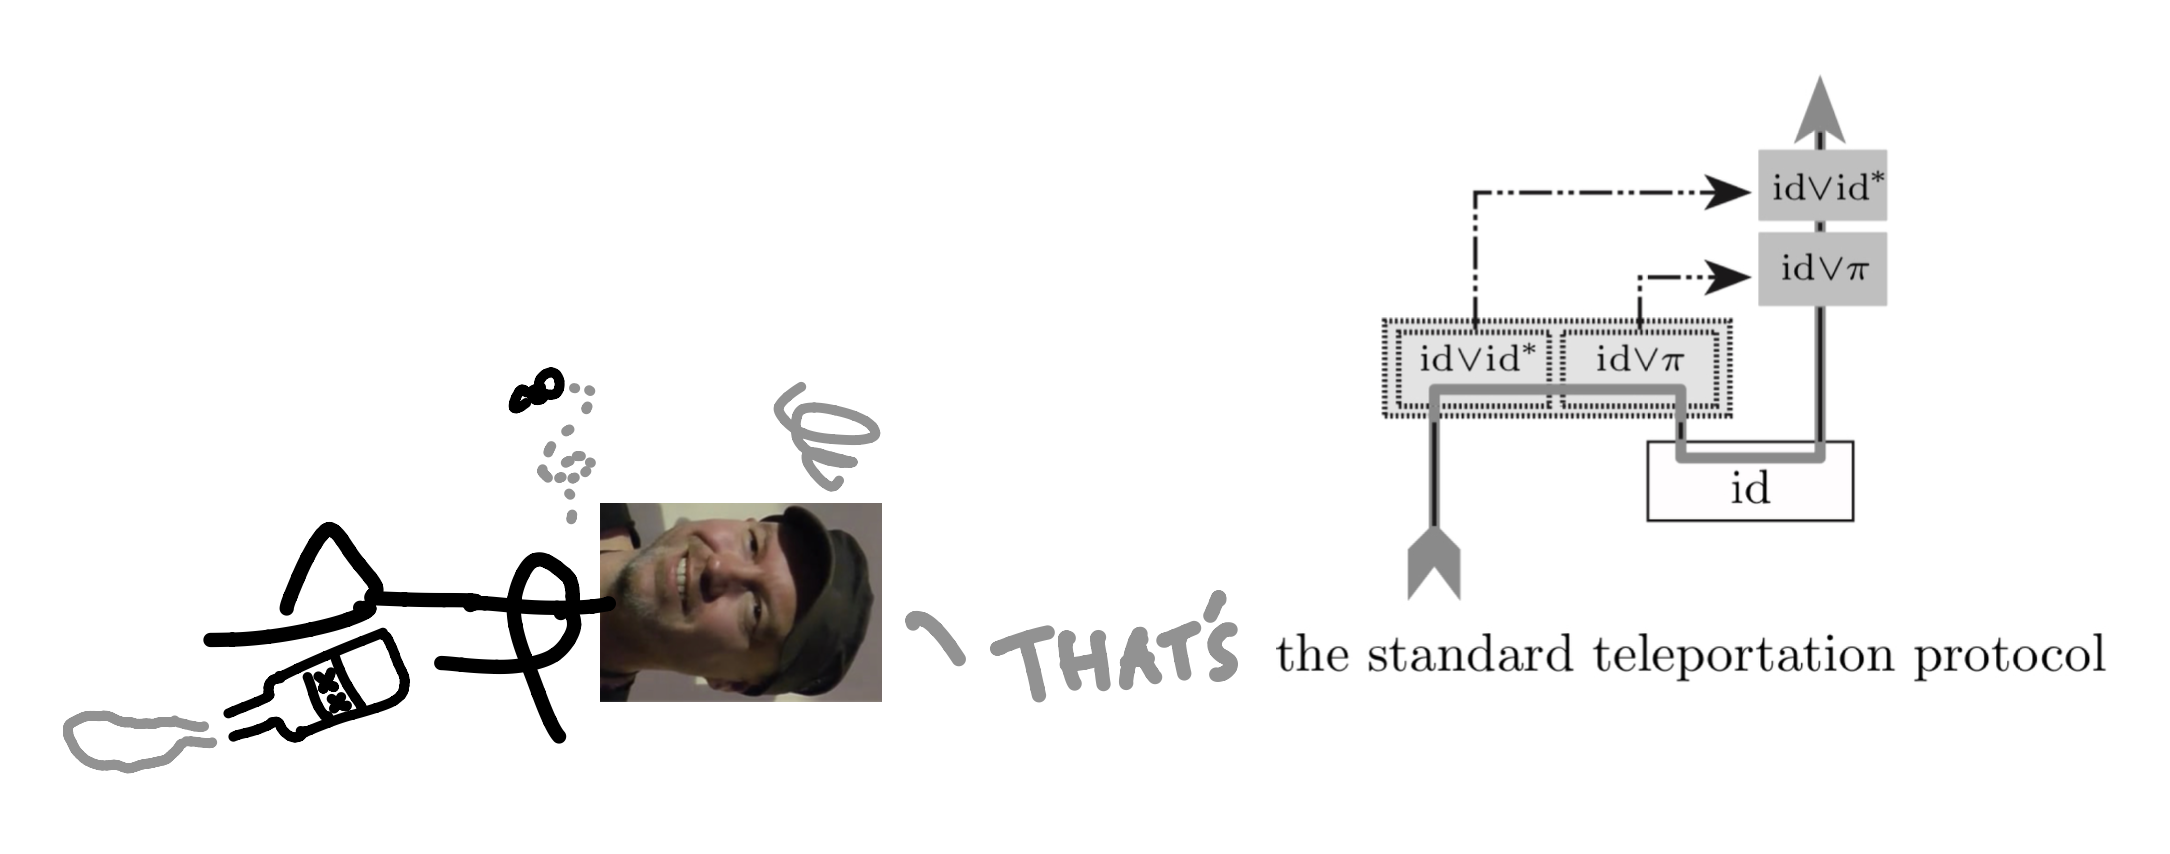
\includegraphics{figures/cartoons/bob2}}
\caption{There were two impressive things about these diagrams. First, the effects such as transparencies for text boxes and curved serifs for angled arrows give a modern feel, but they were done manually in macdraw, the diagrammatic equivalent of sticks and stones. Second, though the diagrams were informal, they provided a way to visualise and reason about entanglement that was impossible by staring at the equivalent matrix formulation of the same composite operator. The most important diagram for our story was this one, which captures the information flow of quantum teleportation.}
\end{figure}
\clearpage

\subsection{Categorical quantum mechanics}

\begin{figure}[h!]
\centering
\scalebox{1}{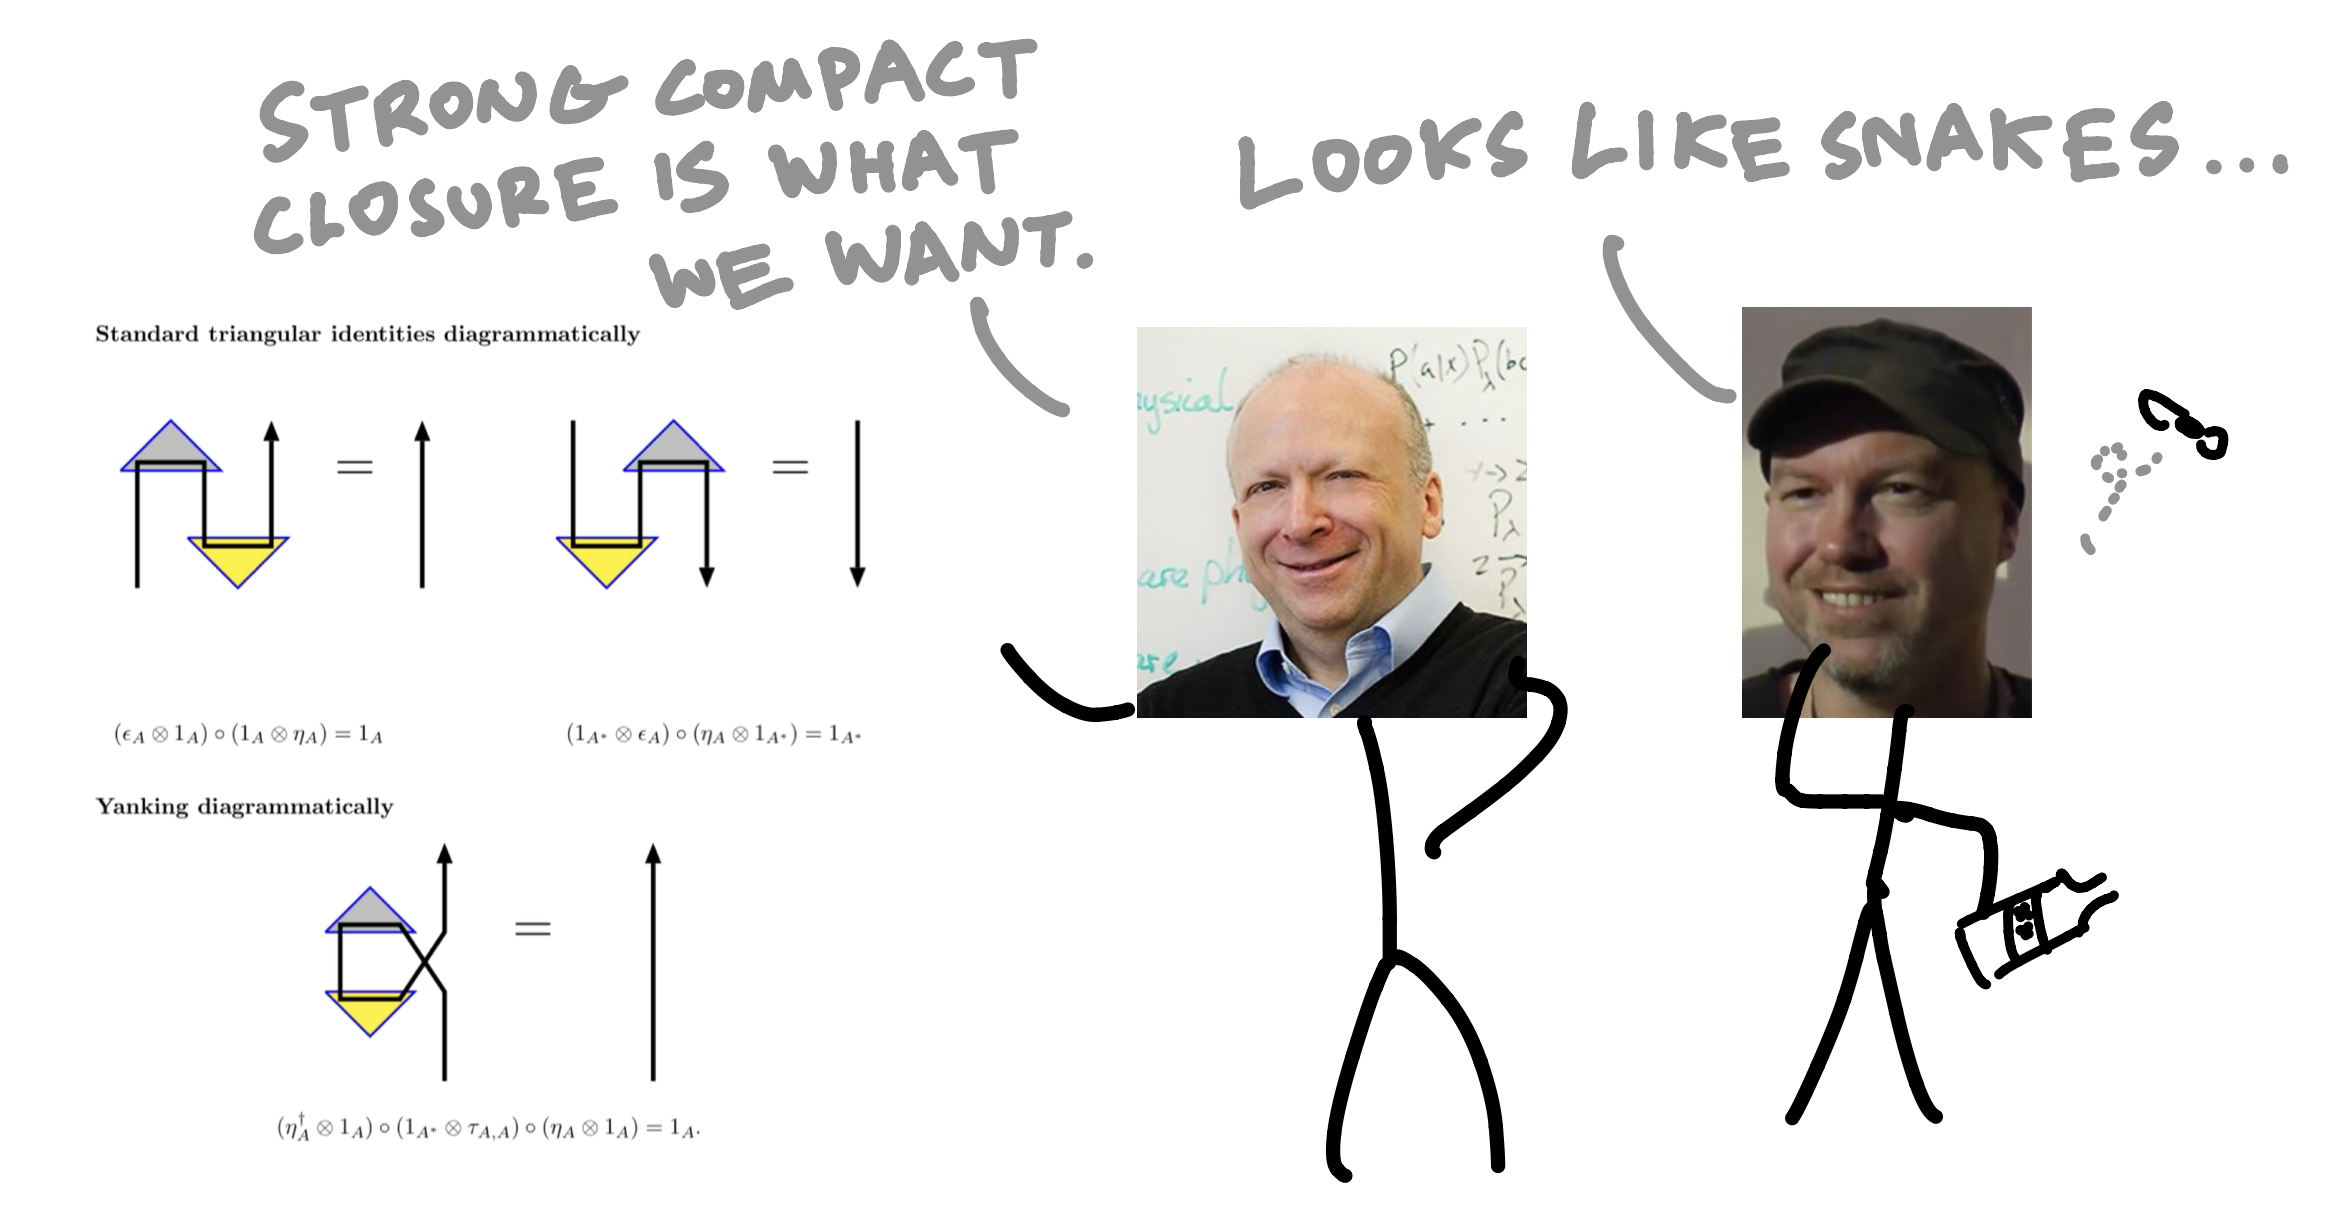
\includegraphics{figures/cartoons/samson}}
\caption{Category theorists and physicists such as Abramsky and Baez were excited about these diagrams, which looked like string diagrams waiting to be made formal. The graphical cups and caps in the important diagram were determined to correspond to a special form of symmetric monoidal closed category called strong compact closed.}
\end{figure}

\begin{figure}[h!]
\centering
\scalebox{1}{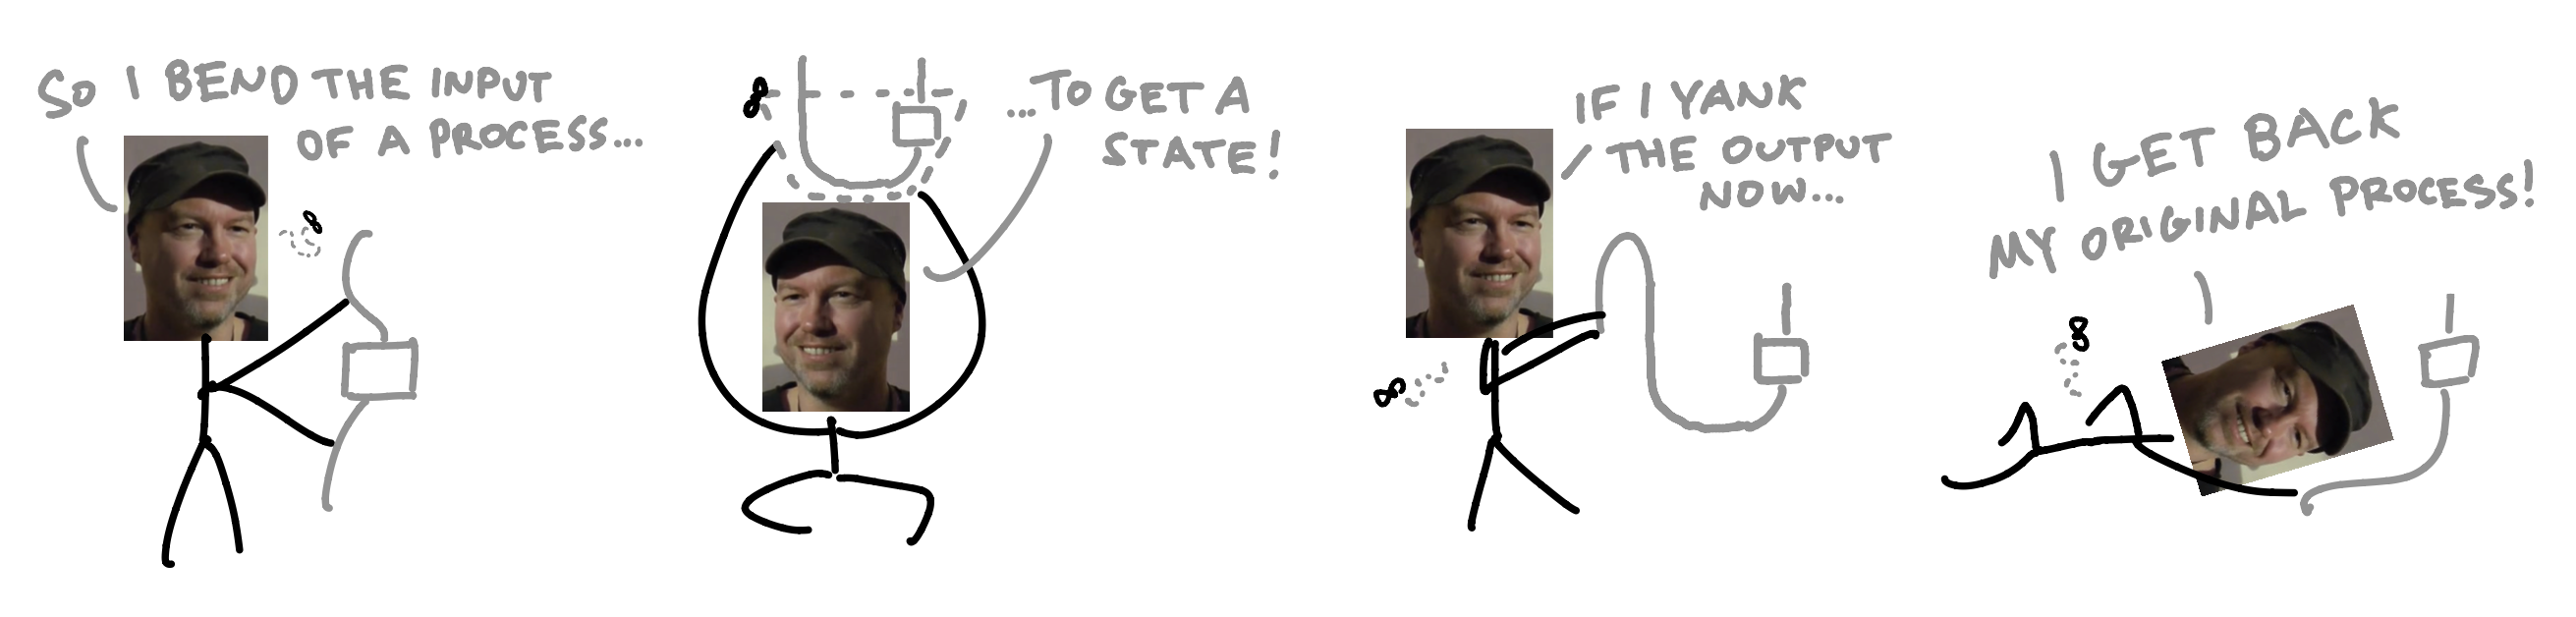
\includegraphics{figures/cartoons/cjiso}}
\caption{Diagrammatically, reasoning in a strongly compact closed category amounts to ignoring the usual requirement of processiveness and forgetting the distinction between inputs and outputs, so that "future" outputs could curl back and be "past" inputs. This formulation also gave insight into the structure of quantum mechanics. For example, the process-state duality of strong compact closure manifested as the Choi–Jamiołkowski isomorphism.}
\end{figure}

\begin{figure}[h!]
\centering
\scalebox{1}{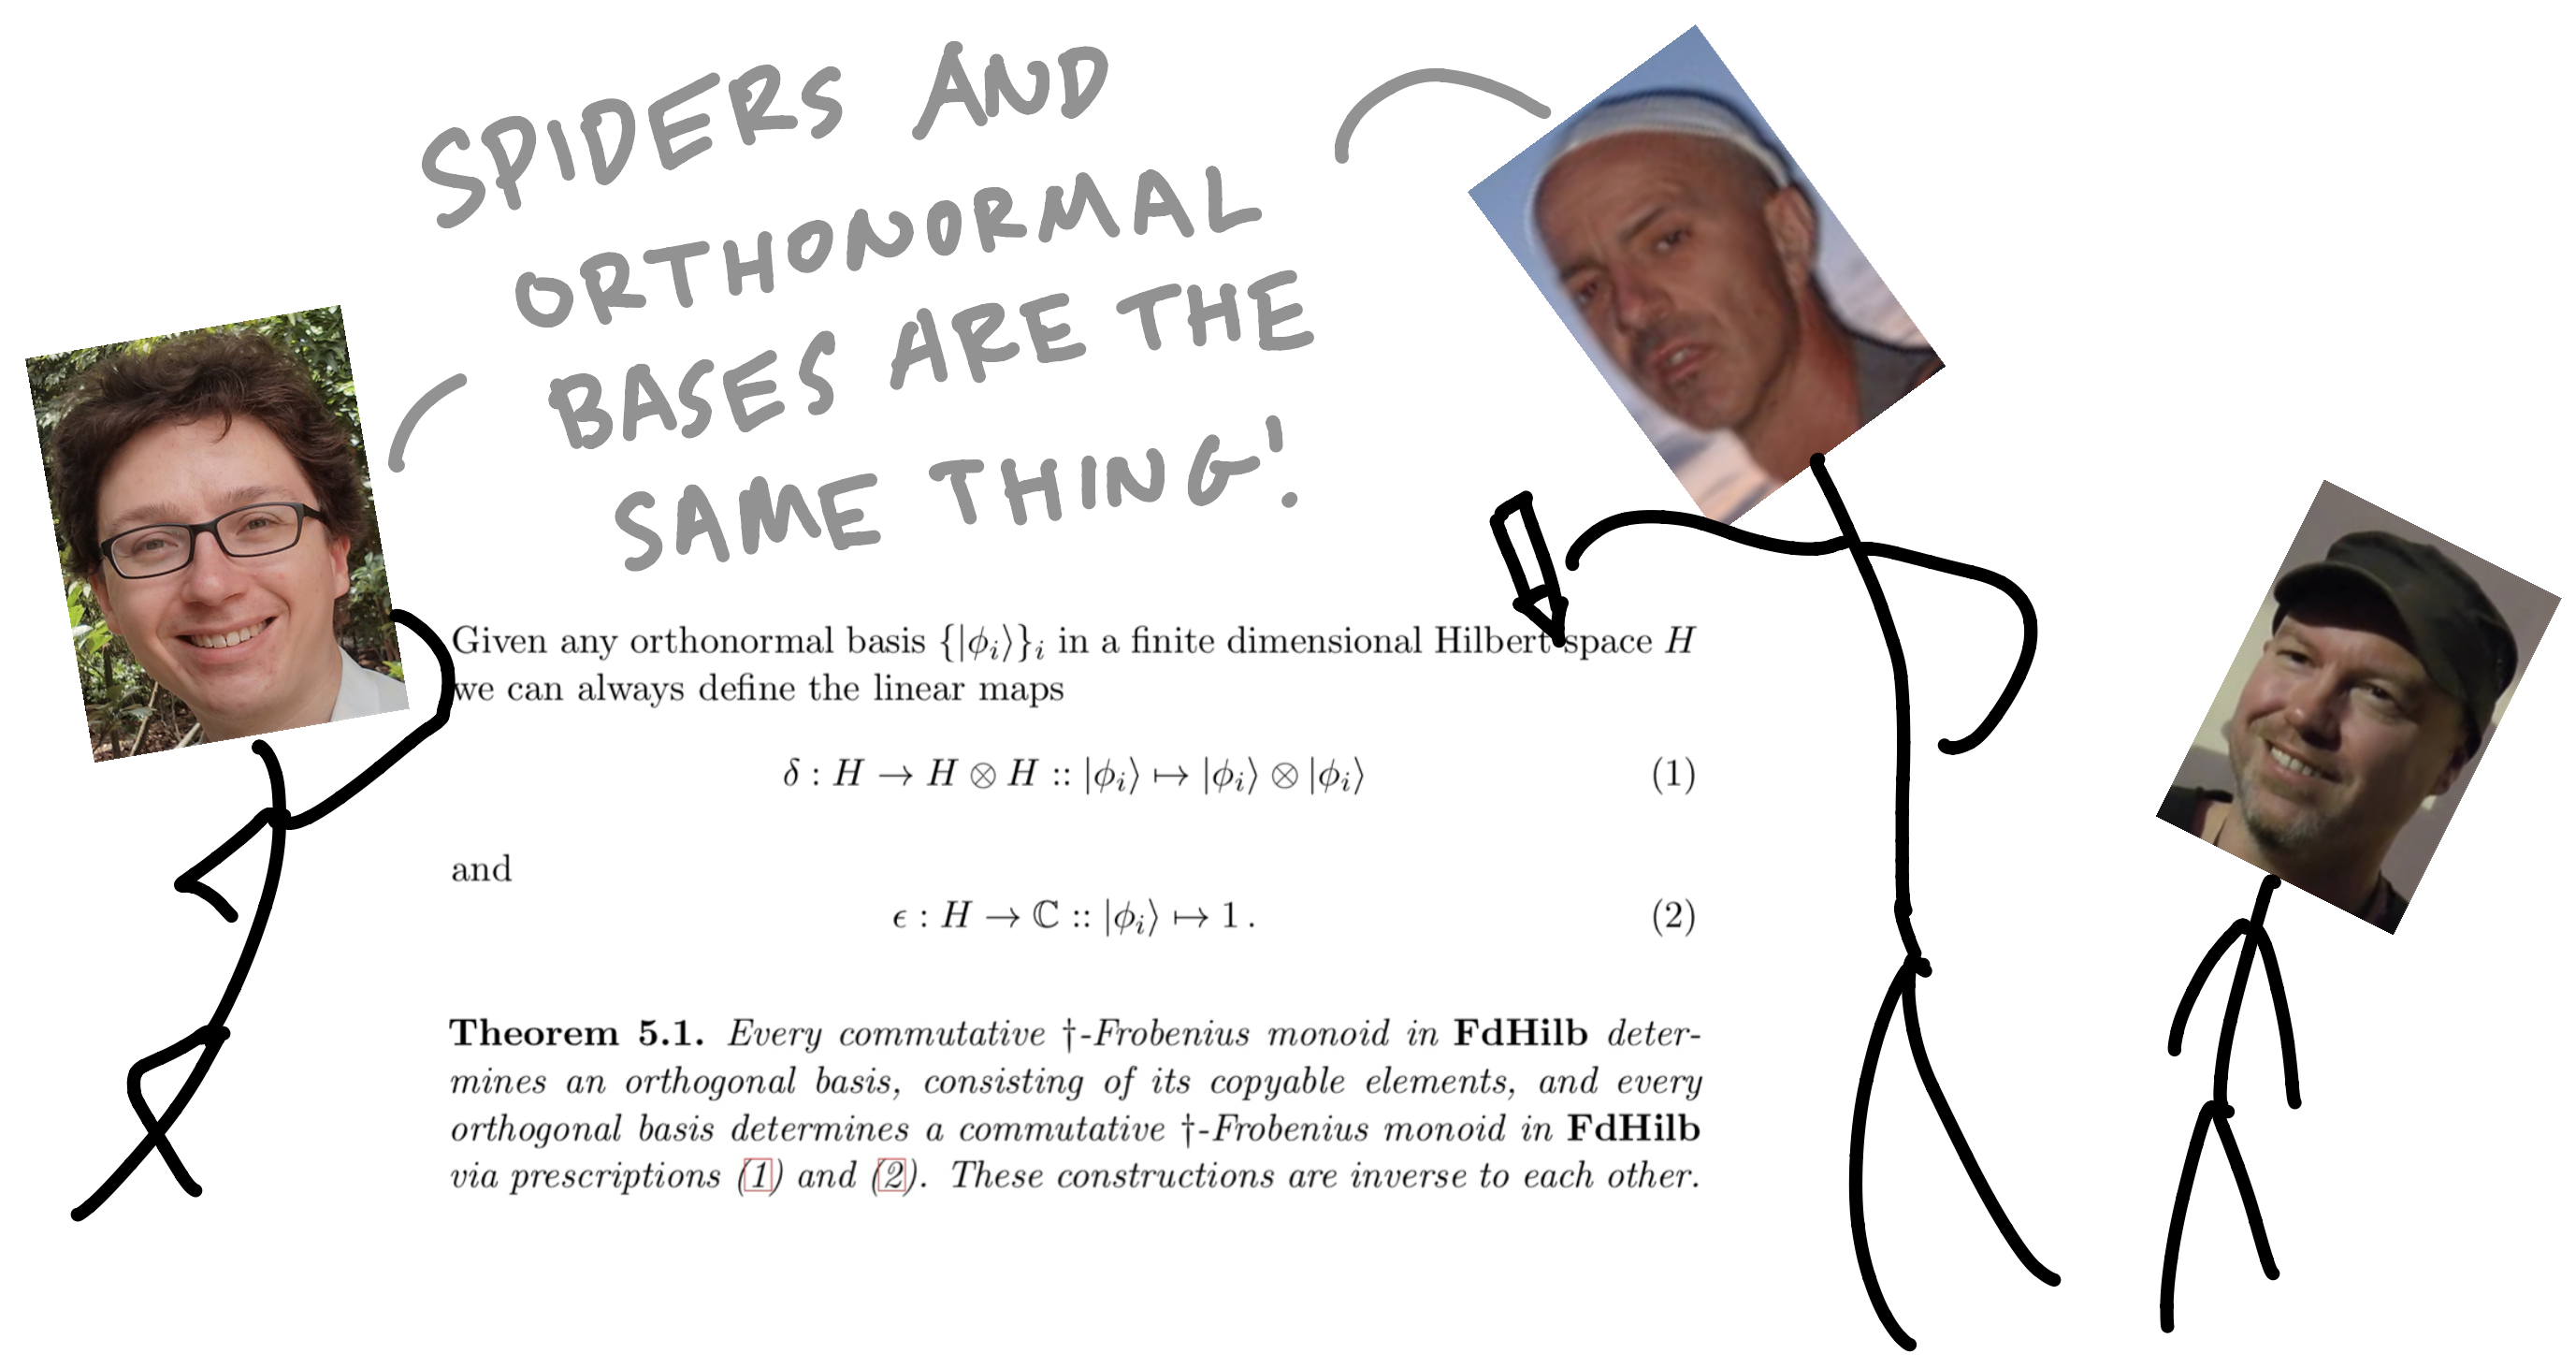
\includegraphics{figures/cartoons/spiders}}
\caption{However, dealing with superpositions necessitated using summation operators within diagrams, which is cumbersome to write especially when dealing with even theoretically simple Bell states. An elegant diagrammatic simplification arose with the observation that special-$\dagger$-frobenius algebras \bR classicquantumstruct \e, or spiders, correspond to choices of orthonormal bases \bR novelchar \e in \textbf{FdHilb}, the ambient setting of finite-dimensional hilbert spaces. Not only did this remove the need for summation operators, it also revealed that strong compact closure was a derived, rather than fundamental structure, since spiders induce compact closed structure.}
\end{figure}

\begin{figure}[h!]
\centering
\scalebox{1}{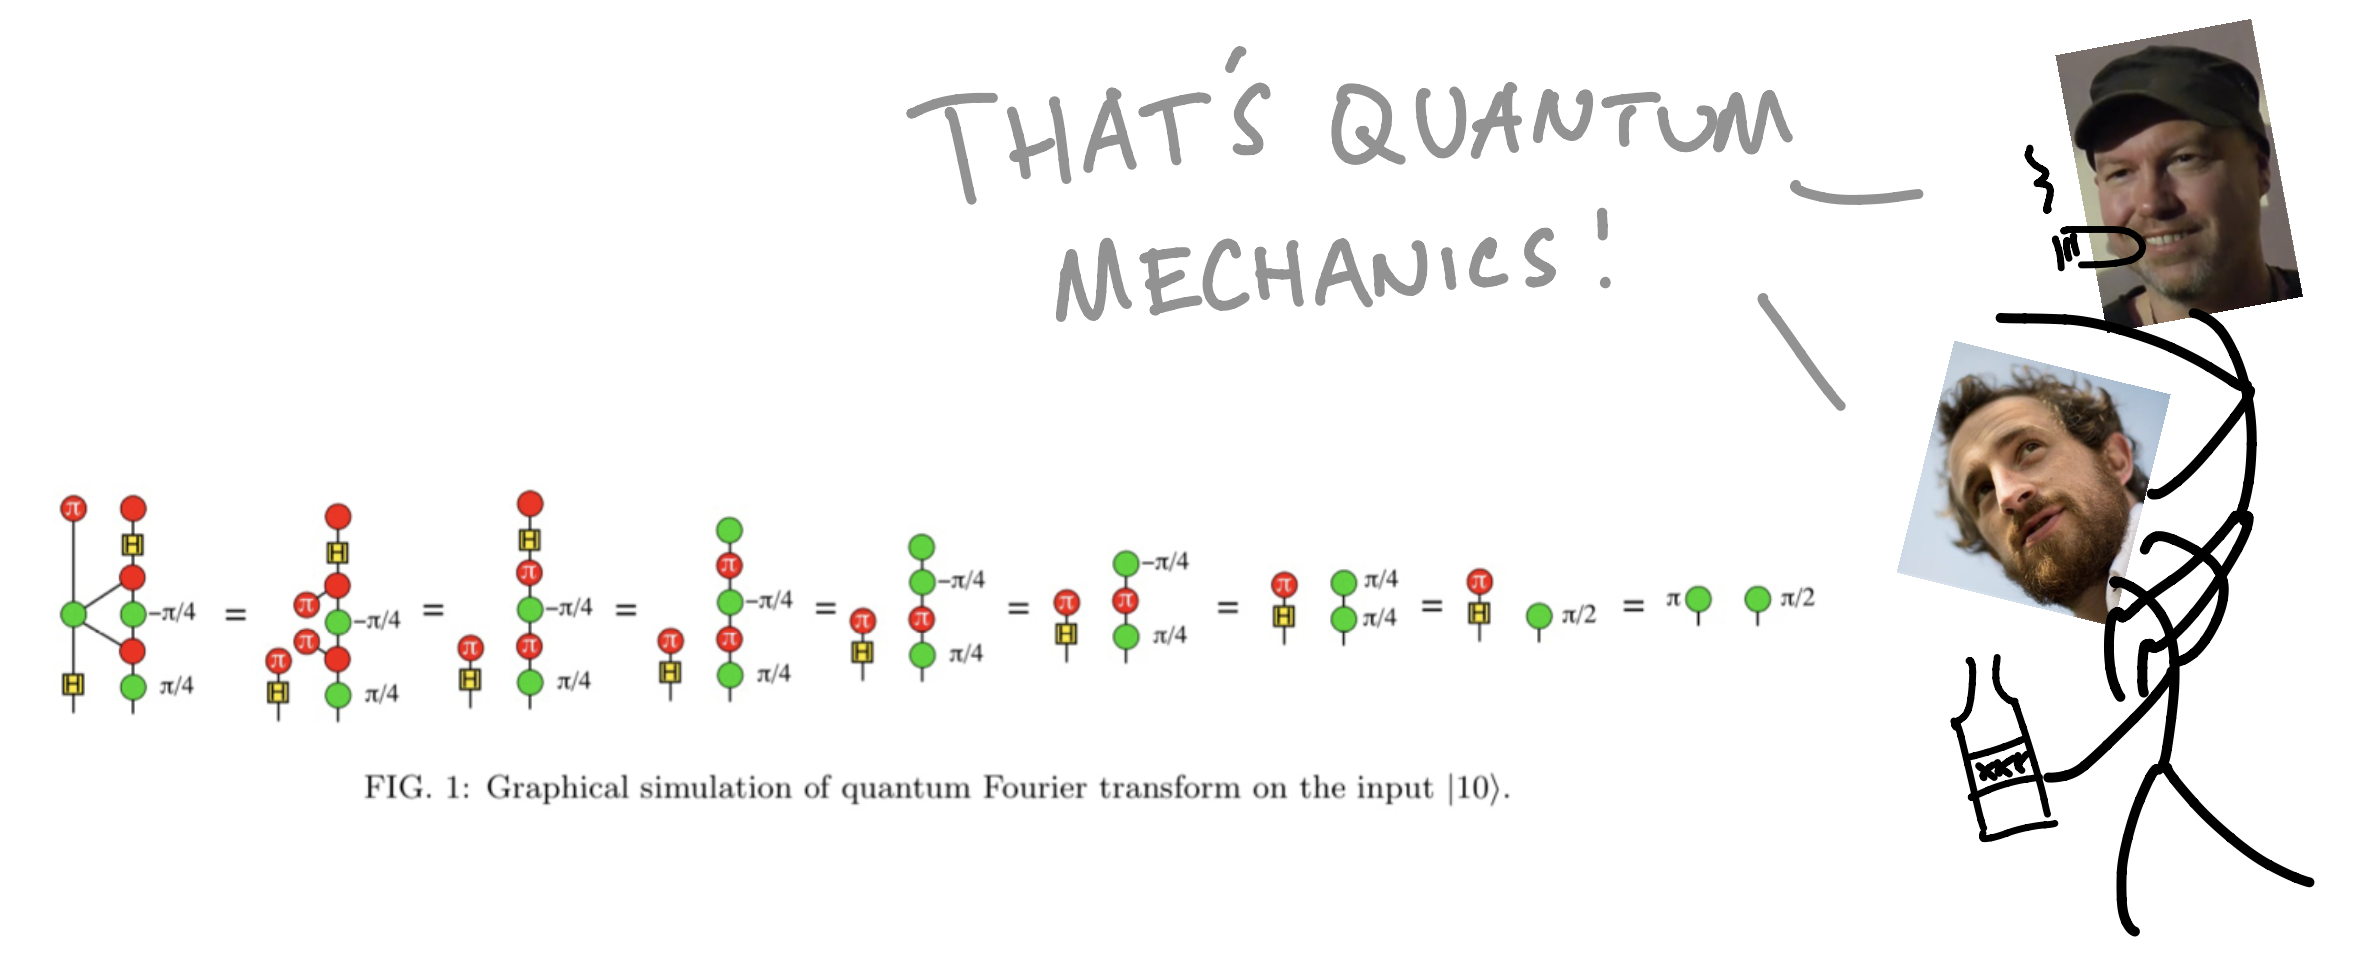
\includegraphics{figures/cartoons/ross}}
\caption{And so the stage was set for a purely diagrammatic treatment of ZX quantum mechanics. The story of ZX diverges away from our interest, so I will summarise what happened afterwards. In no particular order, the development of ZX went on to accommodate a third axis of measurement to yield a ZXW calculus \bR CITE \e, the systems were proven to be complete \bR CITES \e, there are at the time of writing two expository books \bR CITES \e, and ZX-variants are becoming an industry standard for quantum circuit specification and rewriting \bR CITE \e.}
\end{figure}
\clearpage

\subsection{Enter computational linguistics}

\begin{figure}[h!]
\centering
\scalebox{1}{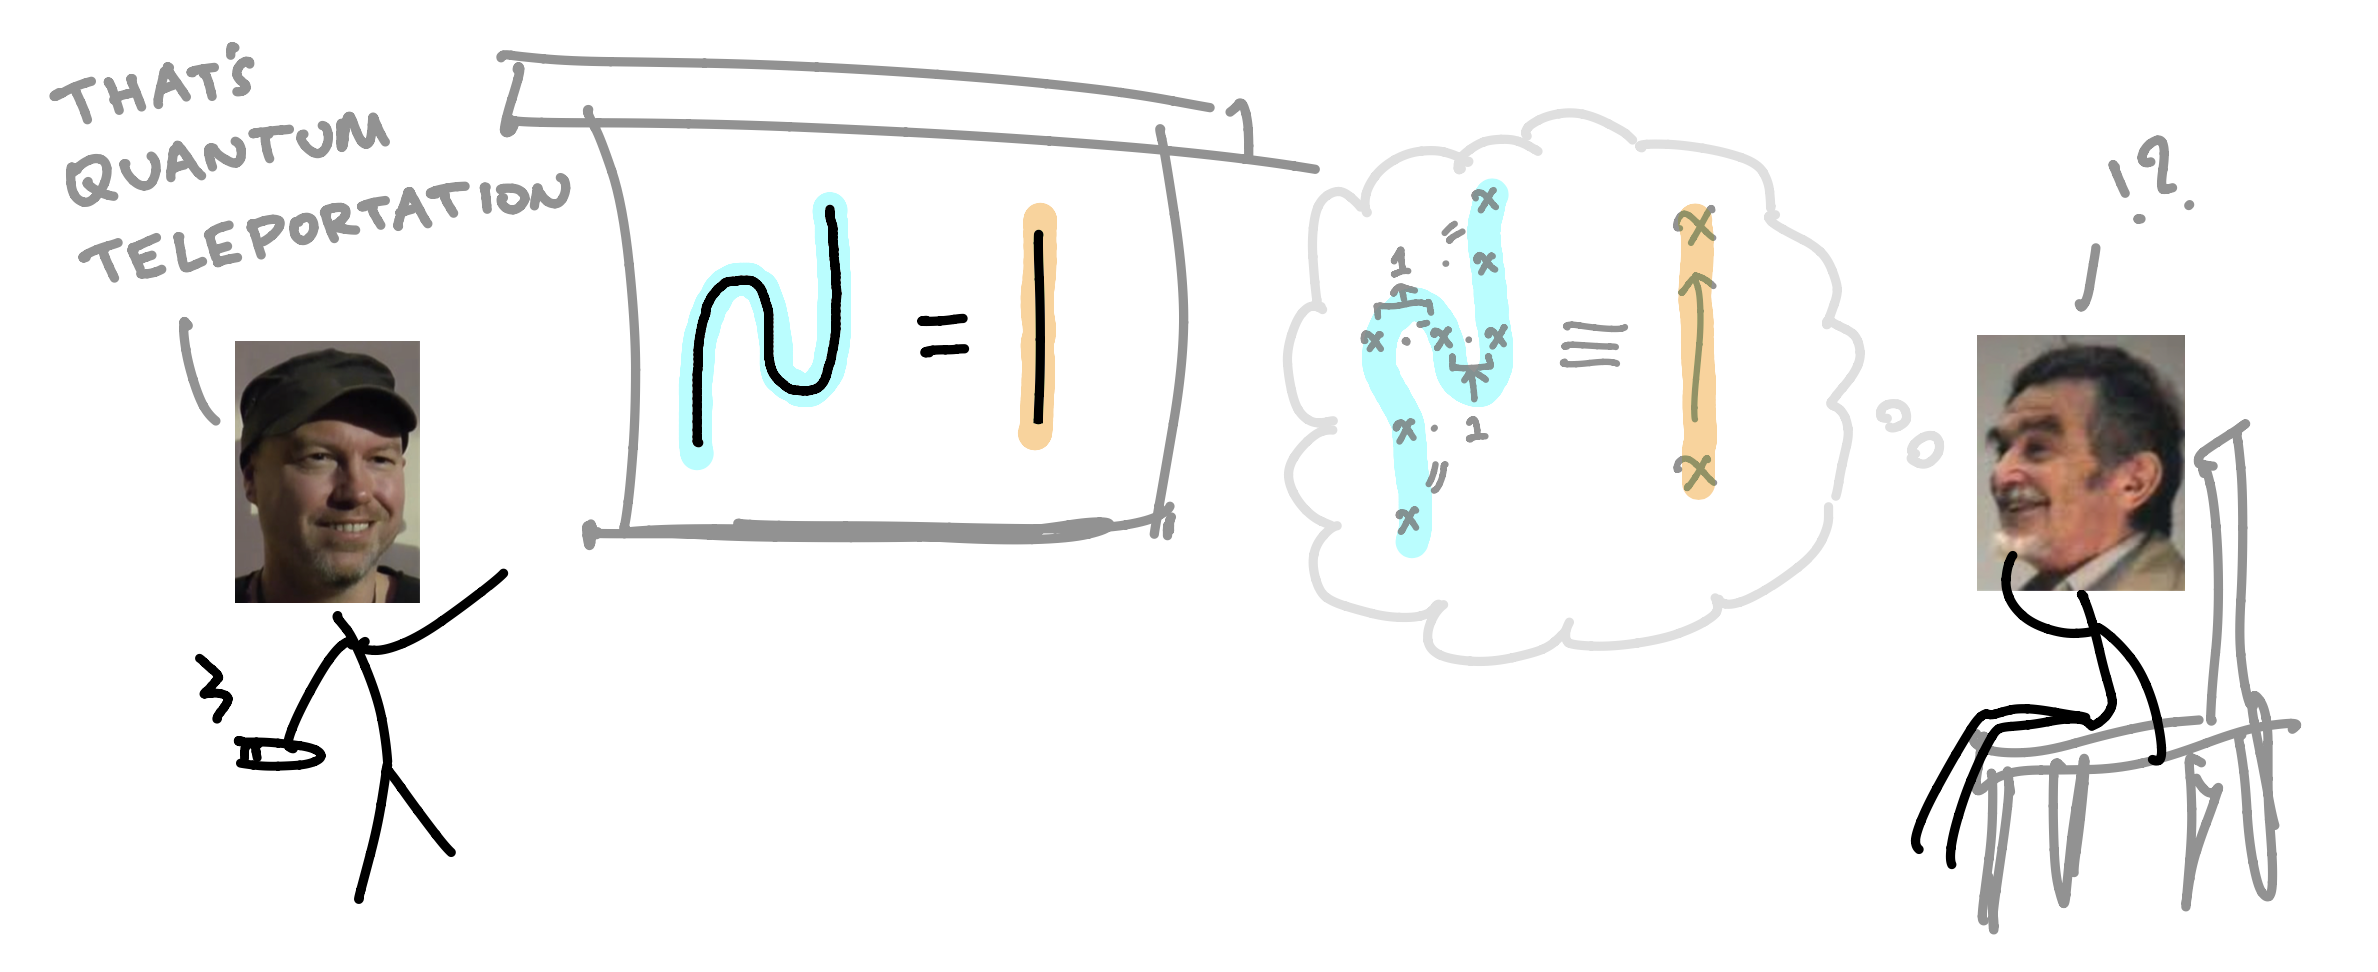
\includegraphics{figures/cartoons/boblambek1}}
\caption{Somewhere in Canada at the turn of the millenium, Bob met Jim, who saw something familiar about the diagram for quantum teleportation. The snake equation for compact closure looked a lot like the categorified version of introducing and eliminating pregroup types.
}
\end{figure}

\begin{figure}[h!]
\centering
\scalebox{1}{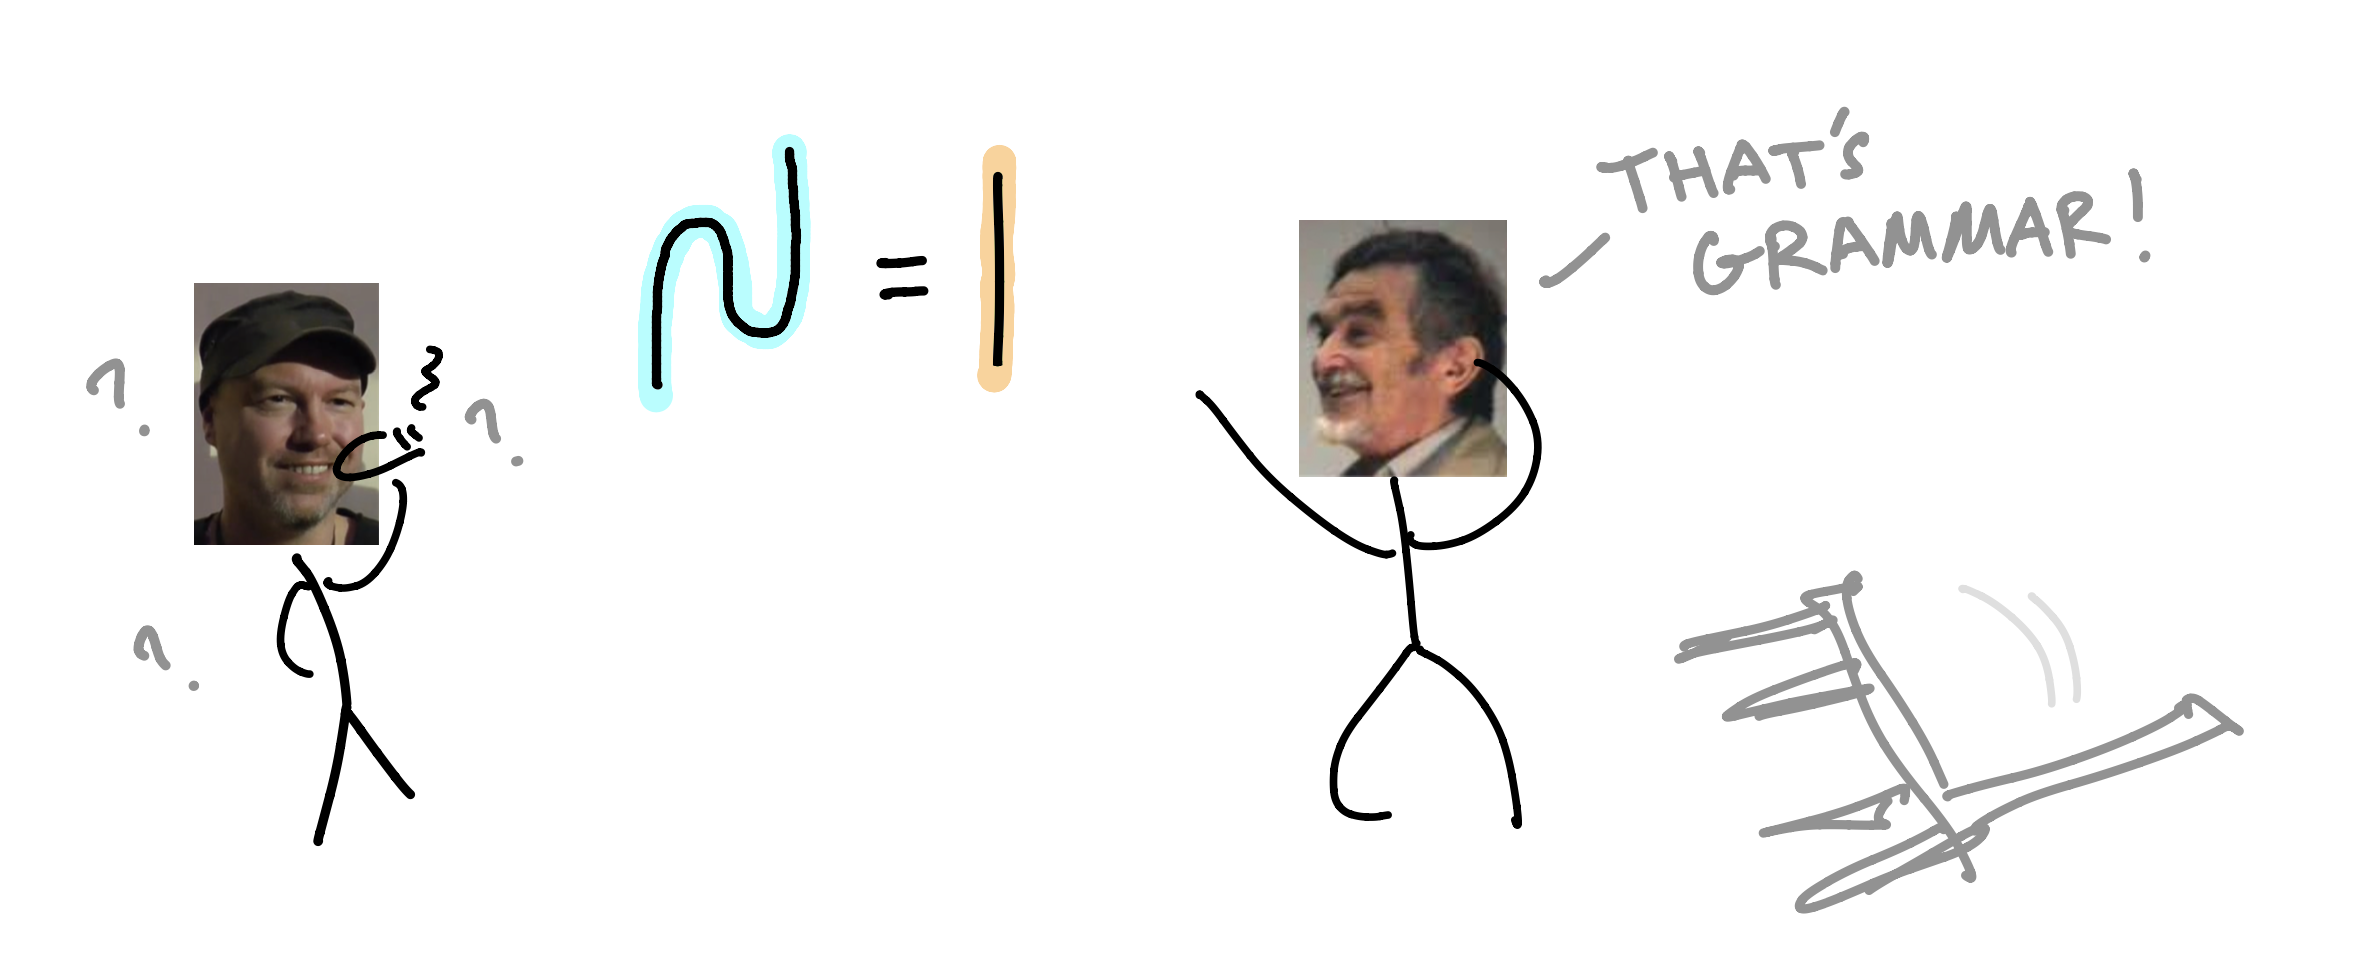
\includegraphics{figures/cartoons/boblambek2}}
\caption{Bob and Jim's meeting put the adjectives \emph{compositional} and \emph{categorical} on the same table, but the cake wasn't ready. Two more actors Steve and Mehrnoosh were required to introduce \emph{distributional}, which refers to Firth's maxim \bR CITE \e "you shall know a word by the company it keeps". In its modern incarnation, this refers generally to vector-based semantics for words, where it is desirable but not necessarily so (as in the case of generic latent space embeddings by an autoencoder) that proximity of vectors models semantic closeness.}
\end{figure}

\begin{figure}[h!]
\centering
\scalebox{1}{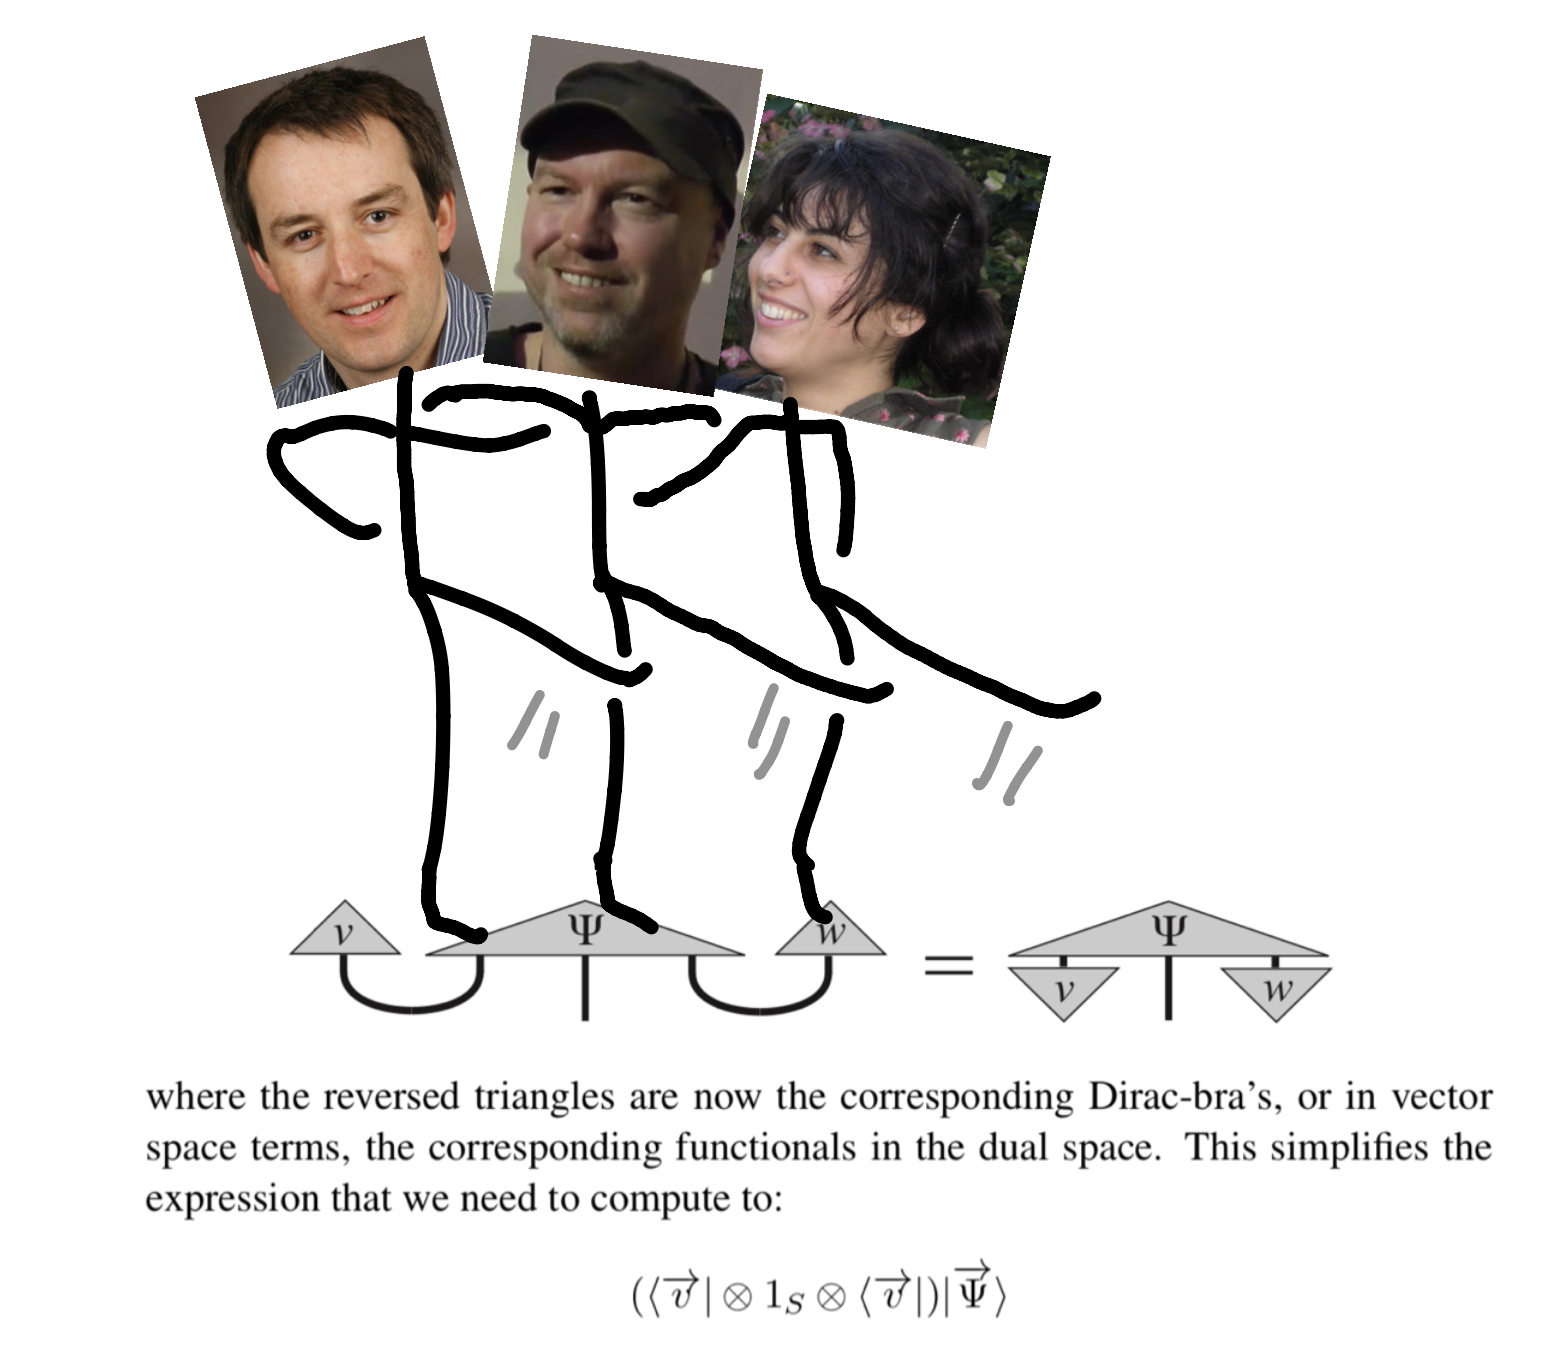
\includegraphics{figures/cartoons/disco1}}
\caption{Steve Clark was a professor in the computer science department at Oxford, and he was wondering how to compose vector-based semantic representations. Steve asked Bob, who realised suddenly what Jim was talking about. Mediated by the linguistic expertise of Mehrnoosh who was a postdoctoral researcher in Oxford at the time, pregroup diagrams were born. The basic types $n$ and $s$ are assigned finite-dimensional vector spaces, concatenation of types the kronecker product $\otimes$, and by the isomorphism of dual spaces in finite dimensions there is no need to keep track of the left- and right- inverse data. Words become vectors, and pregroup reductions become bell-states, or bell-measurements, depending on whether one reads top-down or bottom-up. There was simply no other game in town for an approach to computational linguistics that combined linguistic compositionality with distributional representations.}
\end{figure}

\begin{figure}[h!]
\centering
\scalebox{1}{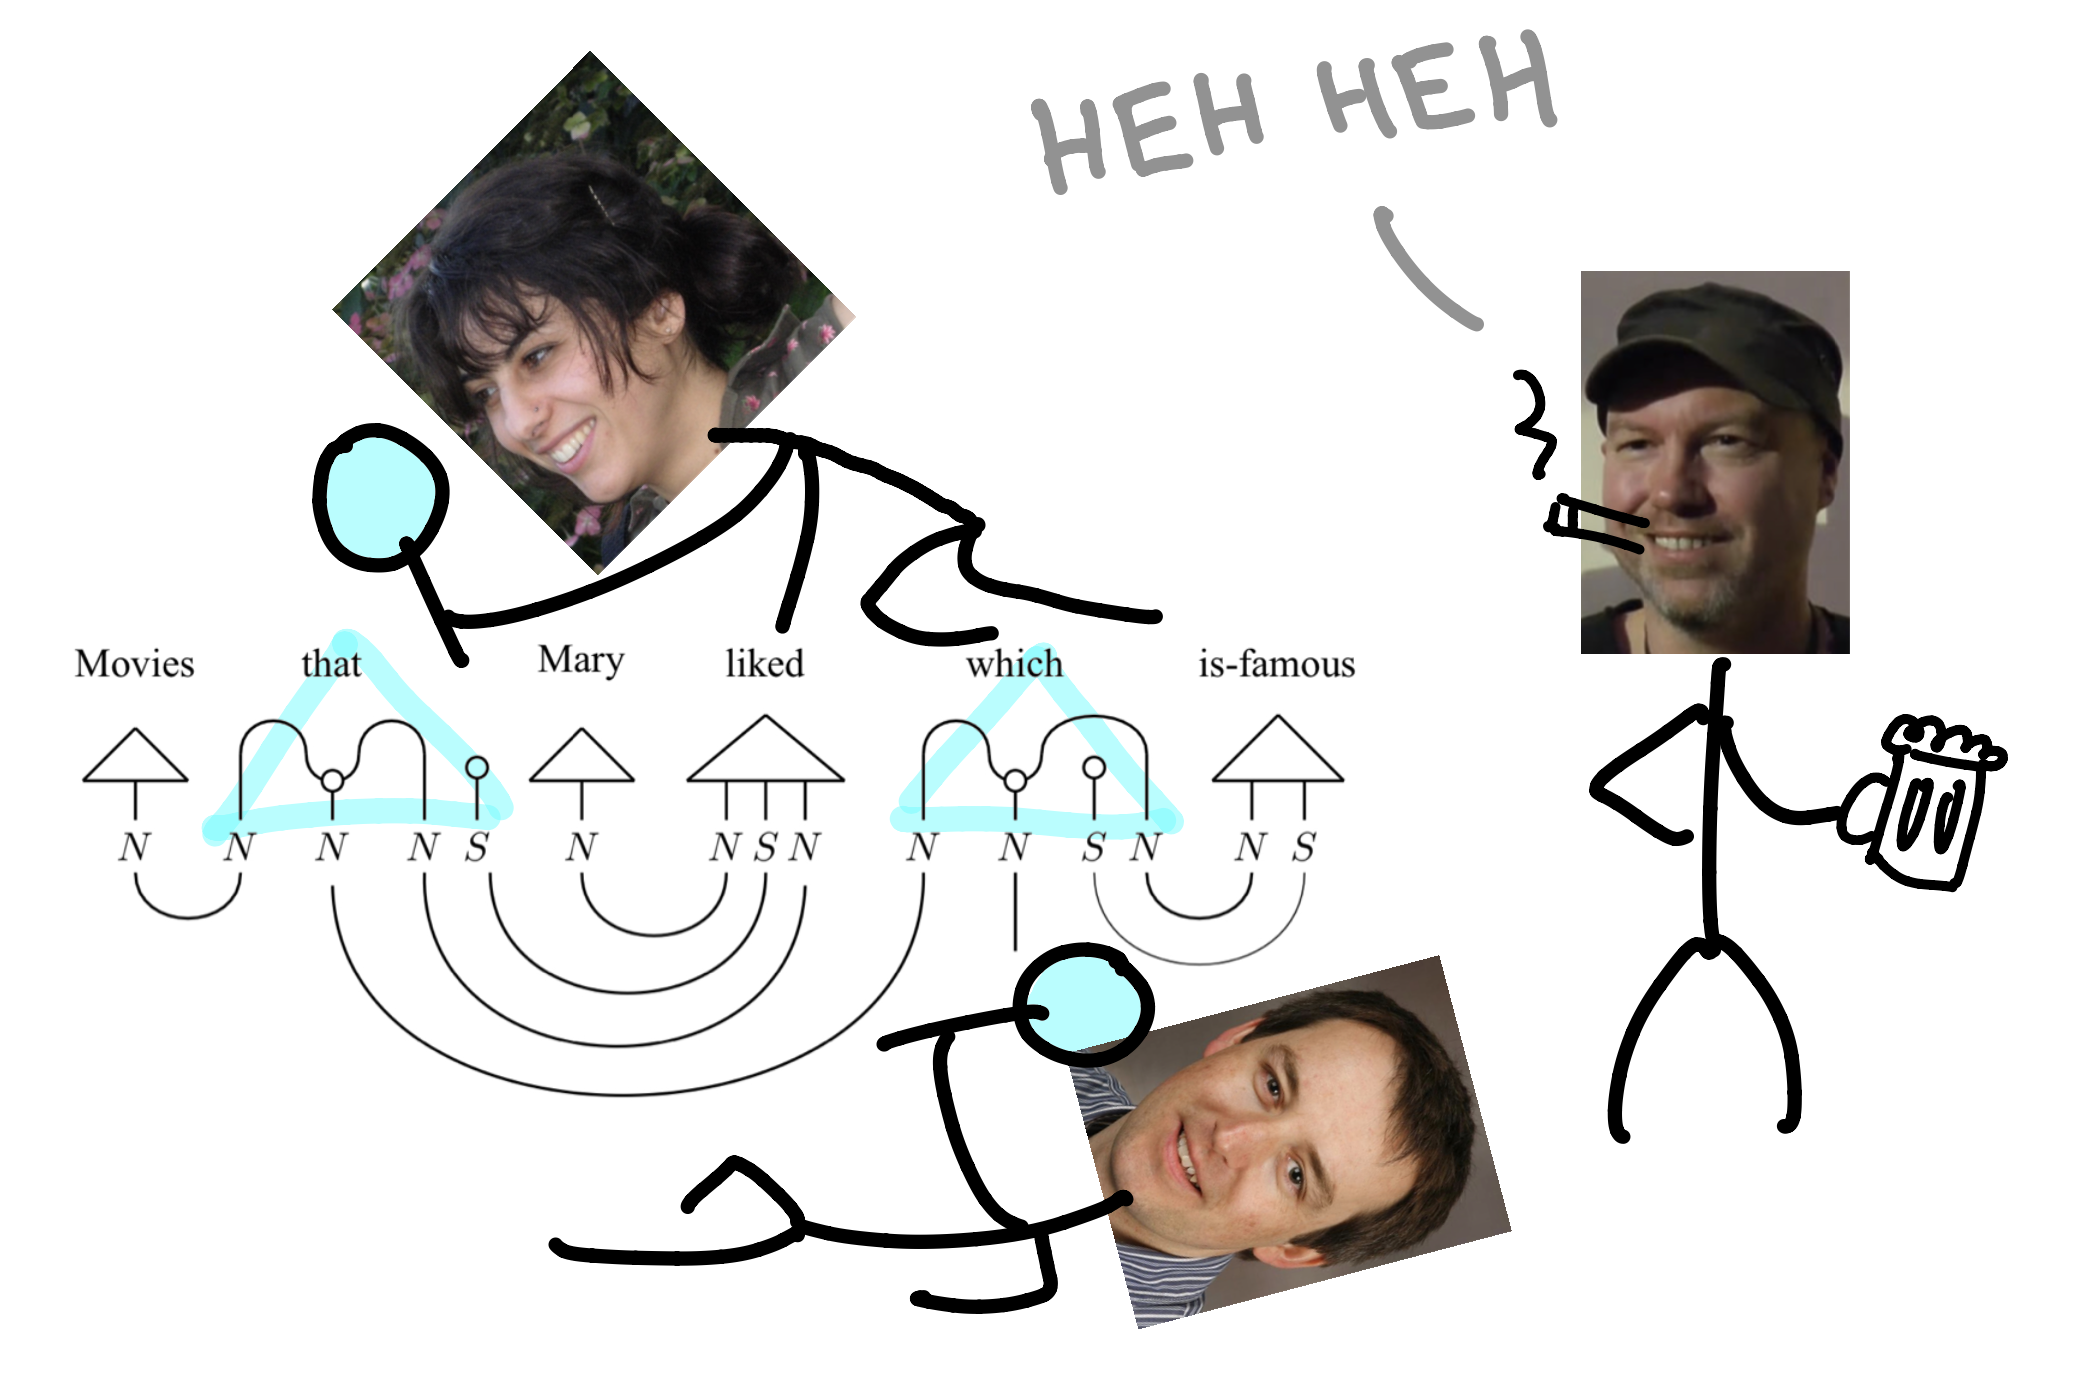
\includegraphics{figures/cartoons/disco2}}
\caption{In \emph{the frobenius anatomy of relative pronouns}\bR CITE \e, the trio realised that spiders could play the role of relative pronouns, which was genuinely novel linguistics. If one follows the noun-wire of "movies", one sees that by declaring the relative pronoun to be a vector made up of a particular bunch of spiders-as-multiwires, "movies" is copied to be related to the "liked" word, copied again by "which" to be related to the "is-famous" word, and a third time to act as the noun in the whole noun-phrase. This discovery clarified a value proposition: insights from quantum theory could be applied in the linguistic setting, and linguistics offered a novel use-case for quantum computers. For example, density matrices were used to model semantic ambiguity \bR CITE \e, and natural language experiments were performed on real quantum computeres \bR CITE \e.}
\end{figure}

\begin{figure}[h!]
\centering
\scalebox{1}{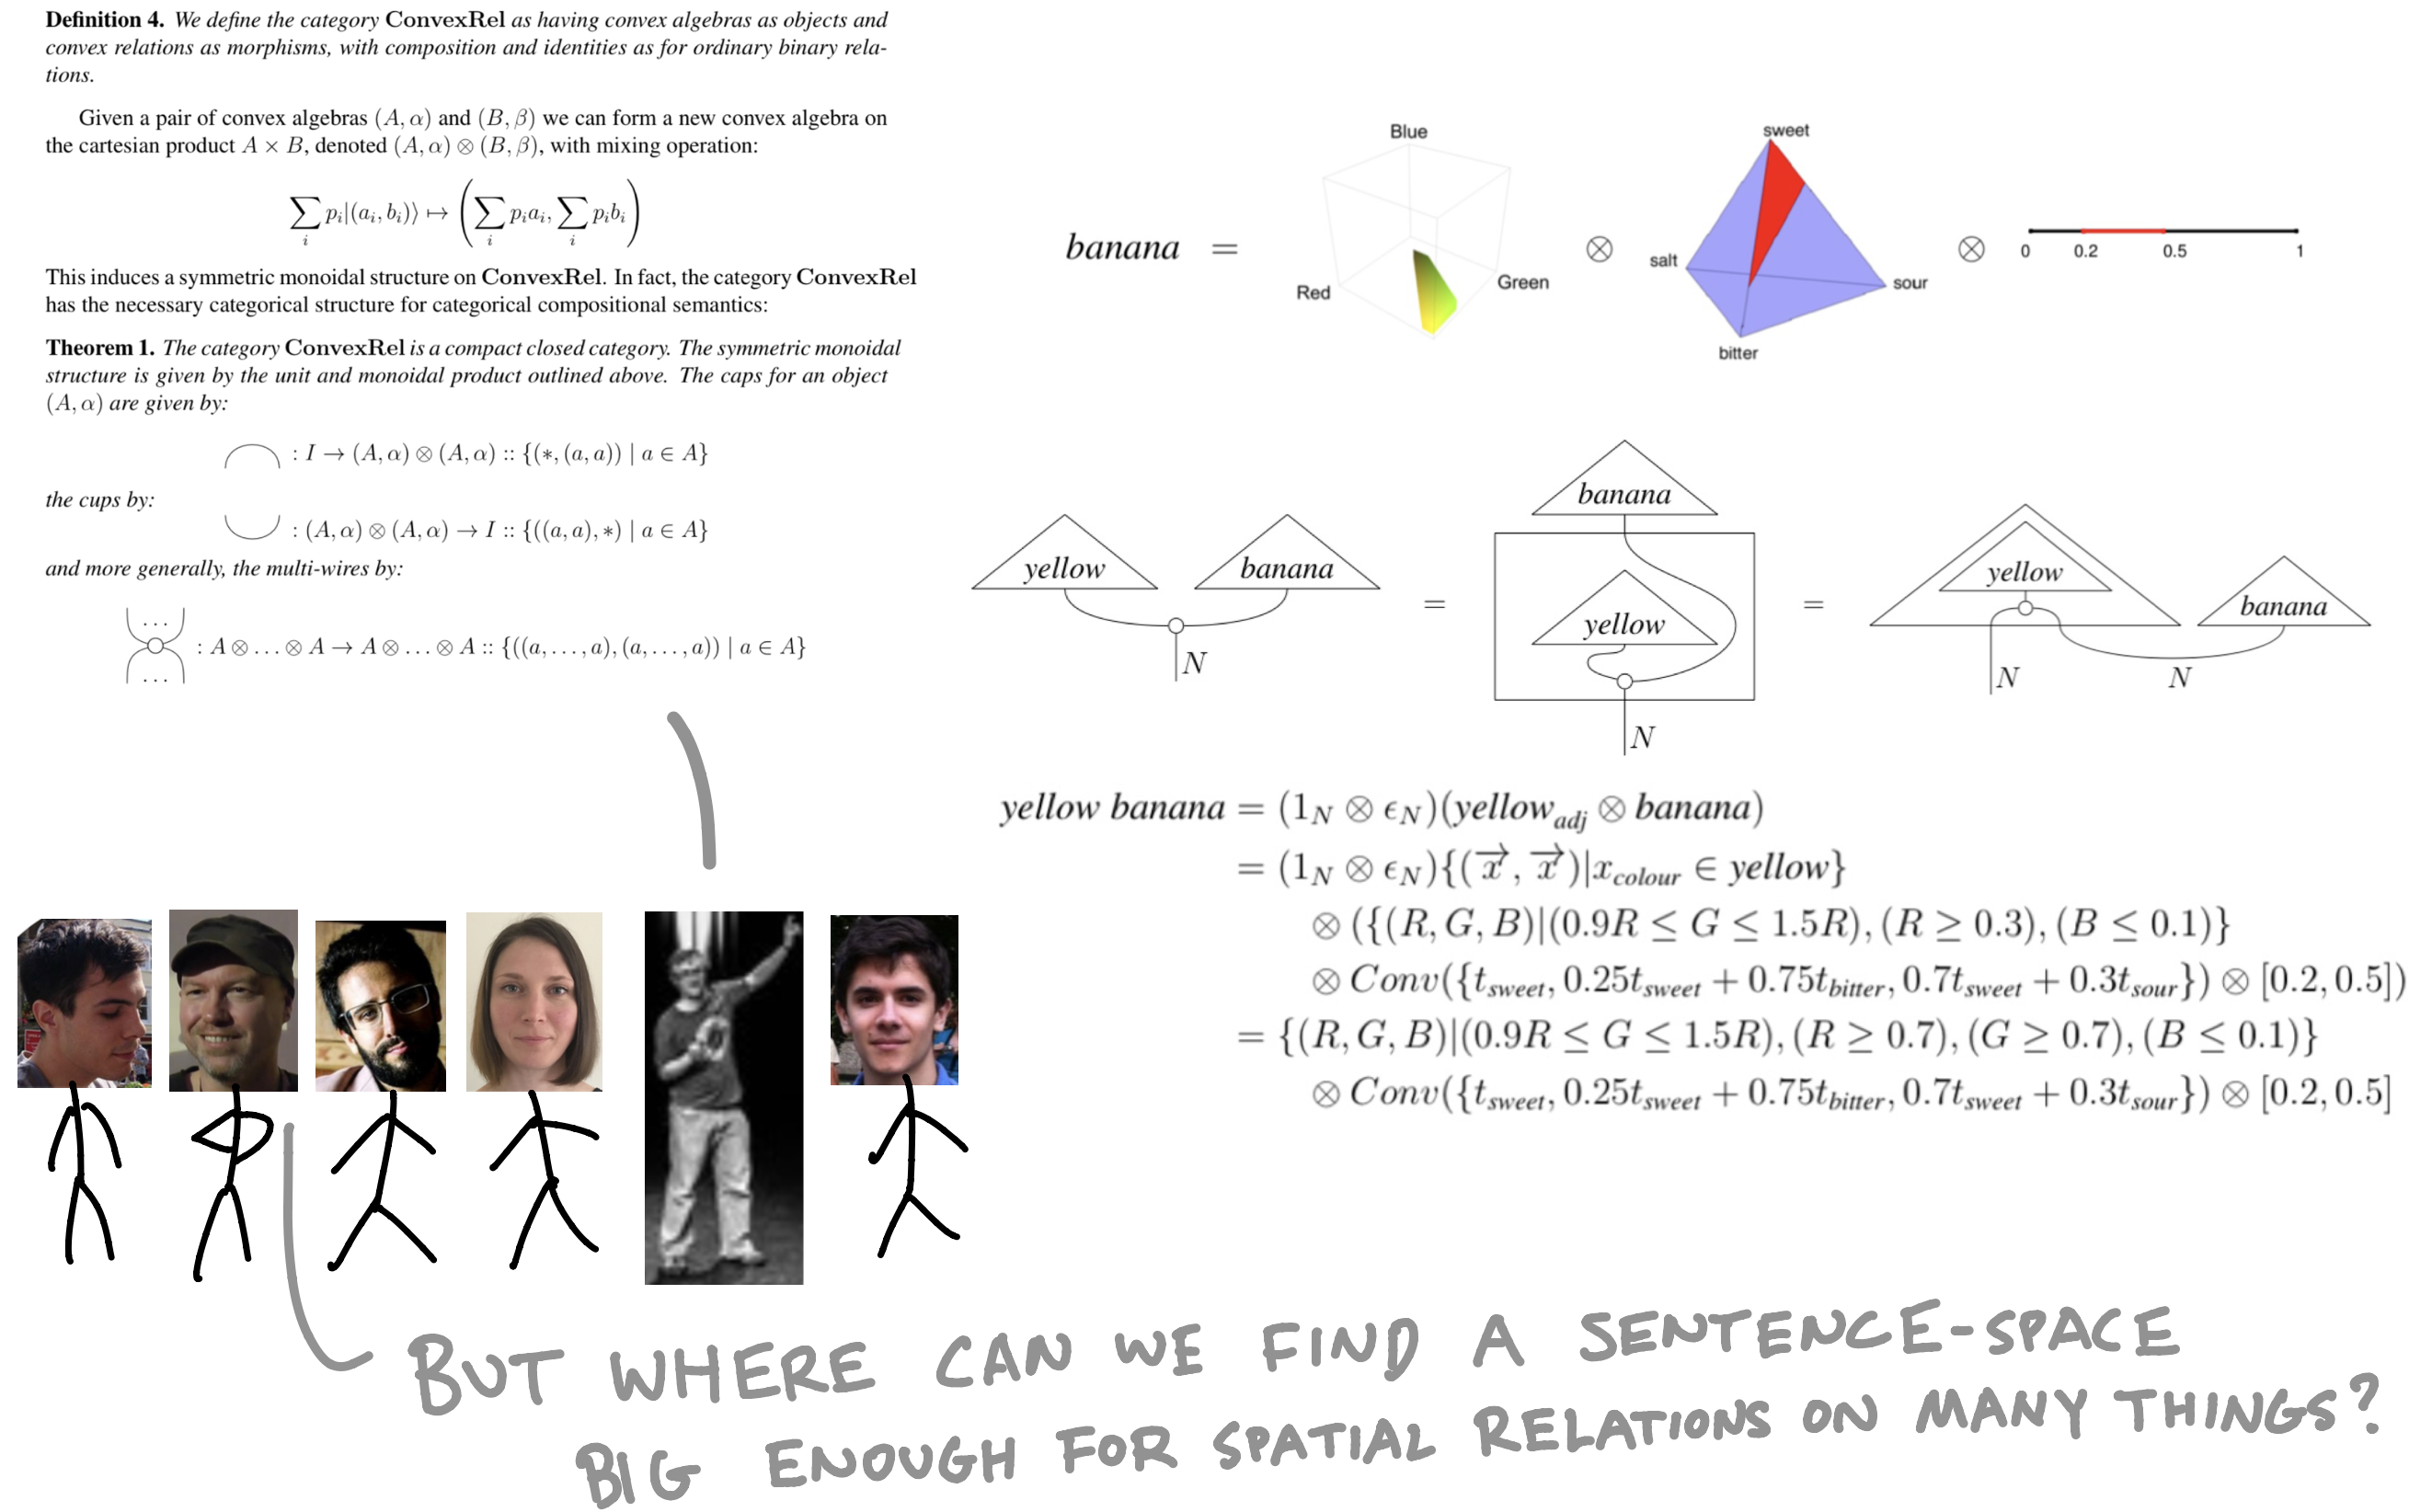
\includegraphics{figures/cartoons/disco3}}
\caption{Keeping the structure of the diagrams but seeking set-relational rather than vector-based semantics, a bridge was made between linguistics and cognitive science in \emph{interacting conceptual spaces I}\bR CITE \e. Briefly, G\"{a}rdenfors posits that spatial representations of concepts mediate raw sense data and symbolic representations -- e.g. red is a region in colourspace -- and moreover that concepts ought to be spatially convex -- e.g. mixing any two shades of red still gives red. This paper created a new point in the value proposition: that new mathematics would arise from investigating the linguistic-quantum bridge, e.g. generalised relations \bR CITE \e. Although labelled as if it is the first in a series, the paper never saw a sequel by the same title, blocked by an apparently simple but actually tricky theoretical problem. The problem is that while this convex-relational story worked for conceptual adjectives modifying a single noun such for "sweet yellow bananas", there was difficulty in extending the story to work for multiple objects interacting in the same space, as in "cup on table in room". It couldn't be worked out what structure a sentence-wire in \textbf{ConvexRel} ought to have in order to accommodate (in principle) arbitrarily many objects and spatial relations between them.\\

DisCoCat then diverges from the story I want to tell. In no particular order, QNLP was done on an actual quantum computer \bR CITE \e, some software packages were written \bR CITE \e, and some art was made \bR CITE \e.}
\end{figure}
\clearpage



\subsection{I killed DisCoCat, and I would do it again.}

\begin{figure}[h!]
\centering
\scalebox{1}{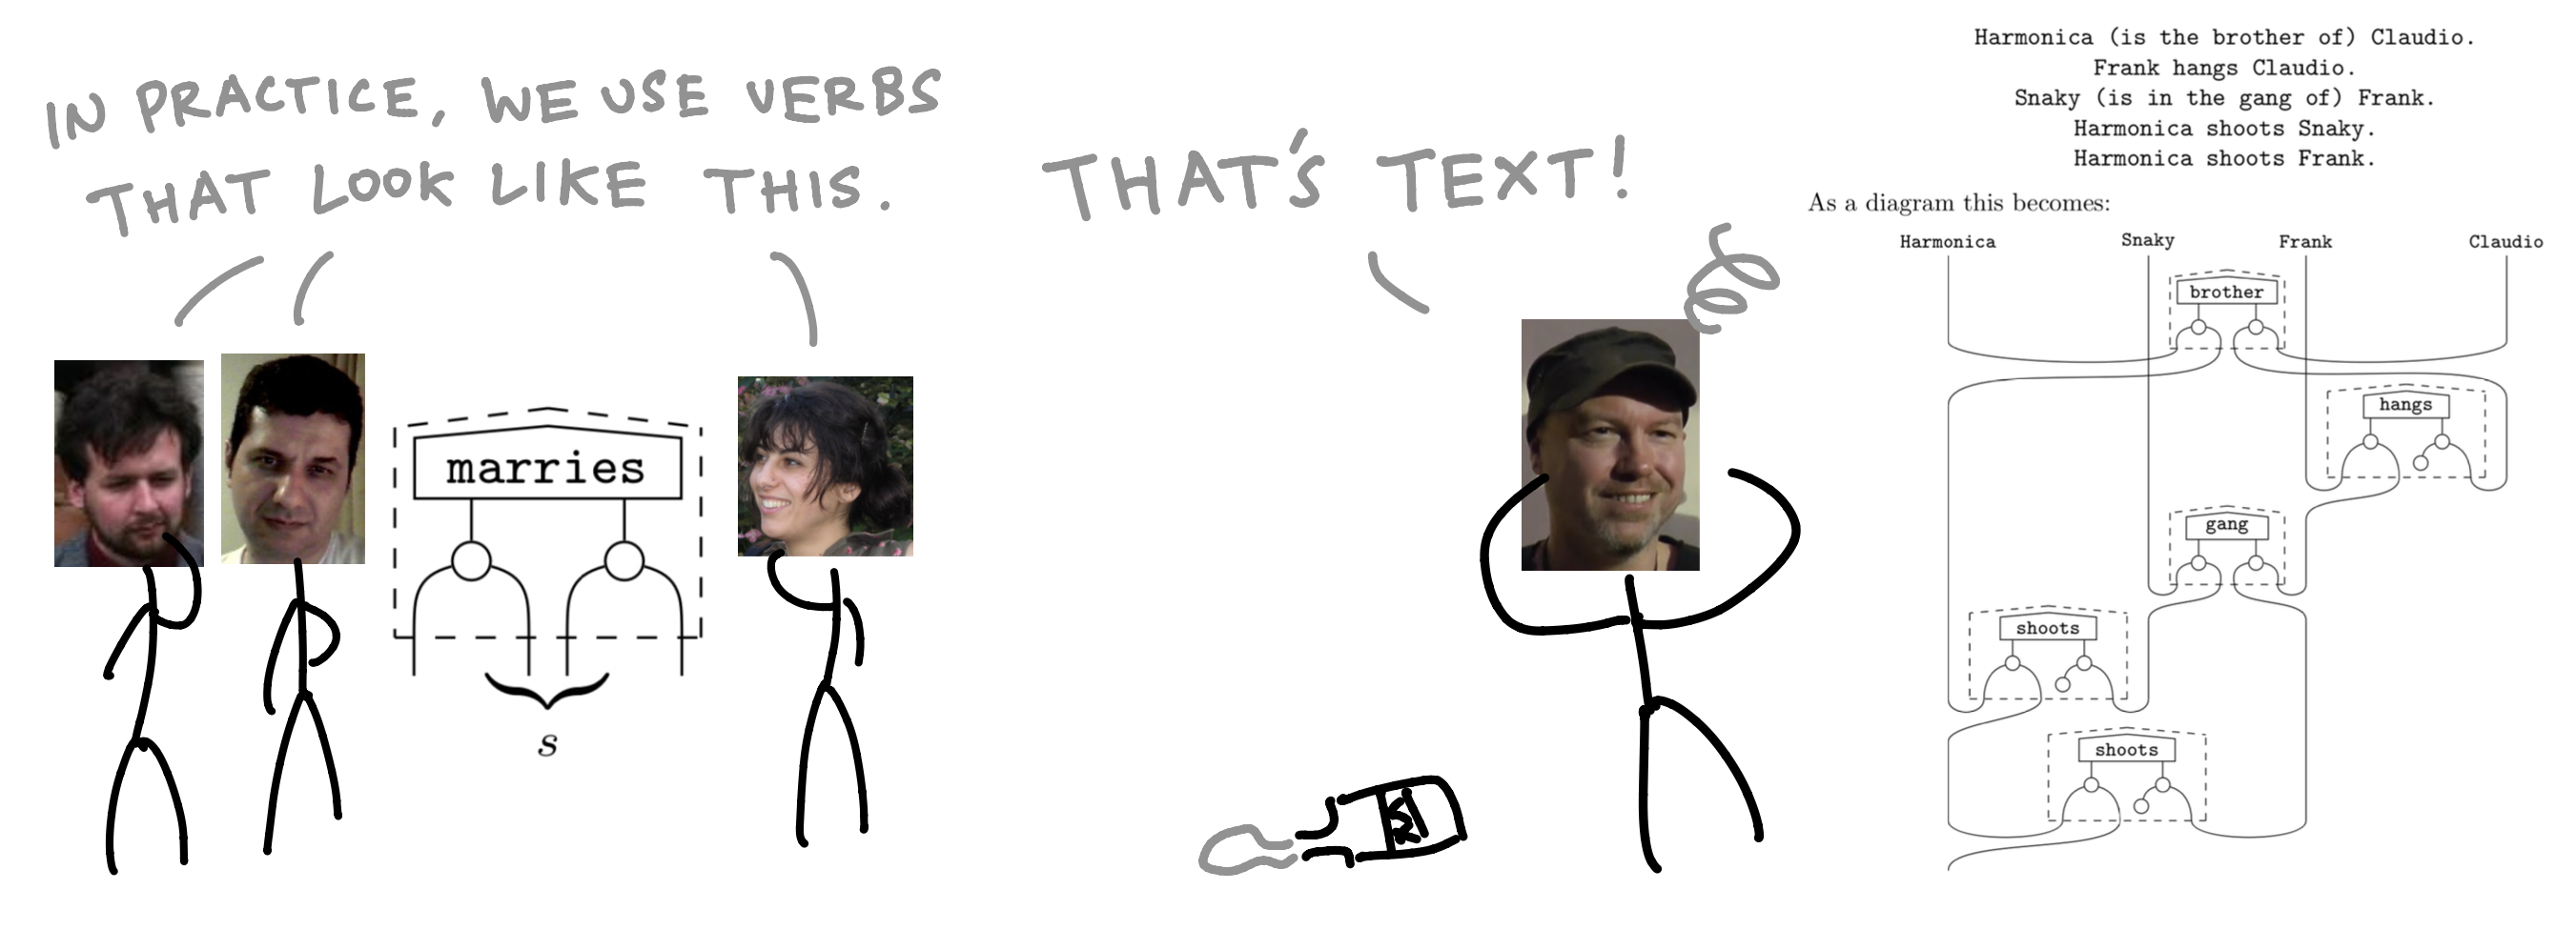
\includegraphics{figures/cartoons/discocirc1}}
\caption{It is a common evolutionary step in linguistics that theories `break the sentential barrier', moving from sentence-restricted to text- or discourse-level analysis \bR CITE \e. The same thing happened with DisCoCirc, due to a combination of practical constraints and theoretical ambition. On the practical side, wide tensors were (and remain) prohibitively expensive to simulate classically and actual quantum computers did not (and still do not) have many qubits, hence in practice pregroup diagrams were reduced to thinner and deeper circuits, often with the help of an additional simplifying assumption that sentence wires were pairs of noun wires in the illustrated form on the left. Theoretically, seeking dynamic epistemic logic, Bob had an epiphanous hangover (really) where he envisioned that these "Cartesian verbs" could be used in service of compositional text meanings, and he called this idea DisCoCirc \bR CITE \e.}
\end{figure}

\begin{figure}[h!]
\centering
\scalebox{1}{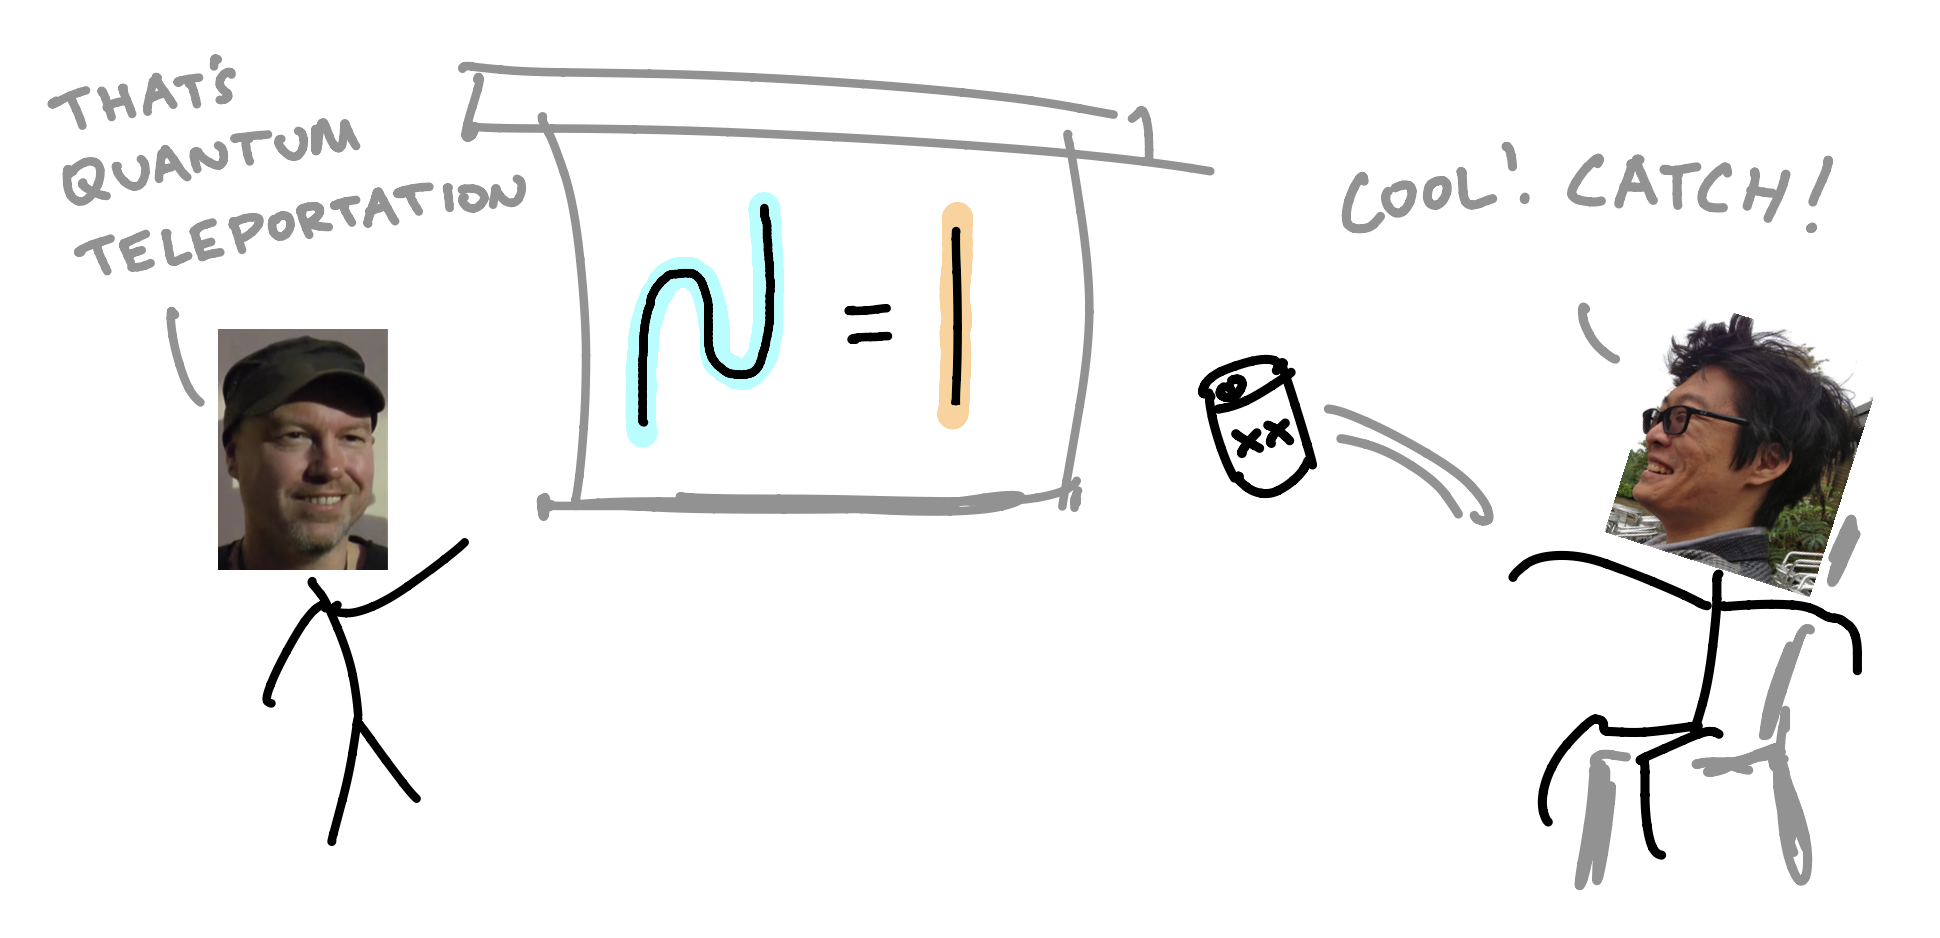
\includegraphics{figures/cartoons/v1}}
\caption{I met Bob in my master's in 2019, where he taught the picturing quantum processes course. When quantum teleportation was explained in half a minute by a diagram, I decided to pursue a DPhil in diagrammatic mathematics. In the last lecture, I threw Bob a cider, after which he seemed to like me. I did not know he was an alcoholic.}
\end{figure}
\clearpage

I was shanghaied into thinking about diagrams for language. I was deeply dissatisfied with the content from the standpoint my own intellectual integrity. Firstly, there seemed to me an unspoken claim that the presence of cups in pregroup diagrams (which implied a noncartesian and hence large tensor product) made it necessary to use quantum computers to effectively compute pregroup diagrams. I just could not believe that my brain required quantum computation to understand language. This implicit claim of kinship between quantum and linguistics was further entrenched by the analysis of the relative pronoun in terms of frobenius algebras, since spiders in $\mathbf{Vect}^\otimes$ were the \emph{sine qua non} of categorical quantum mechanics. The best steelman for spiders I have is that frobenius algebras (which are central to bicategories of relations \bR CITE \e) just happen to be a ubiquitous mathematical structure that are well-suited to express the mathematics of connections, both in language and in quantum.\\

Second, representing the content of a sentence as a vector in a sentence-vector-space did not sit well with me, since this move meant that the only meaningful thing one could do with two sentences was take their inner-product as a measure of similarity. Moreover, I had the theoretical concern that language is in principle indefinitely productive, so one could construct a sentence that marshalled indefinitely many nouns, and at some point for any finite vector space $s$ one would run out of room to encode relationships, or else they would be cramped together in a way that did not suit intuitions about the freedom of constructing meanings using language. I always believed in the existence of a simple, practical, and intuitive categorical, compositional, and distributional semantics; I just didn't believe that the role of quantum -- however helpful or interesting -- was \emph{necessary}.

My first unsatisfactory attempt was in my Master's thesis \bR CITE \e. It had been known for a while that a free autonomous category construction by Delpeuch \bR CITE \e could potentially eliminate some of the cups in pregroup diagrams, yielding what amounted to a method to transform a pregroup diagram into a monoidal string diagram in the shape of a context-free grammar tree. This trick had the limitation that freely adding directed cups and caps to a string diagrammatic signature did not turn a symmetric monoidal category into a (weakly) compact closed one, rather just into a monoidal category where the original wires had braidings, but all the new left and right dual wires did not; this presented difficulties in accounting for iterated duals for higher-order modifiers such as adverbs in grammatical types, and had nothing to say about spiders. I tried to generalise this trick to `freely' adding arbitrary diagrammatic gadgets to string diagrams, but my assessor Samson pointed out that it was nontrivial to determine whether such constructions were faithful. In retrospect the free autonomous completion of a parameterised \bR CITE \e markov category \bR CITE \e is in the ballpark of dequantumfying pregroup diagrams, but I didn't learn about them until later, and that still wouldn't have addressed the issues that come with only having a sentence-wire.

\begin{figure}[h!]
\centering
\scalebox{1}{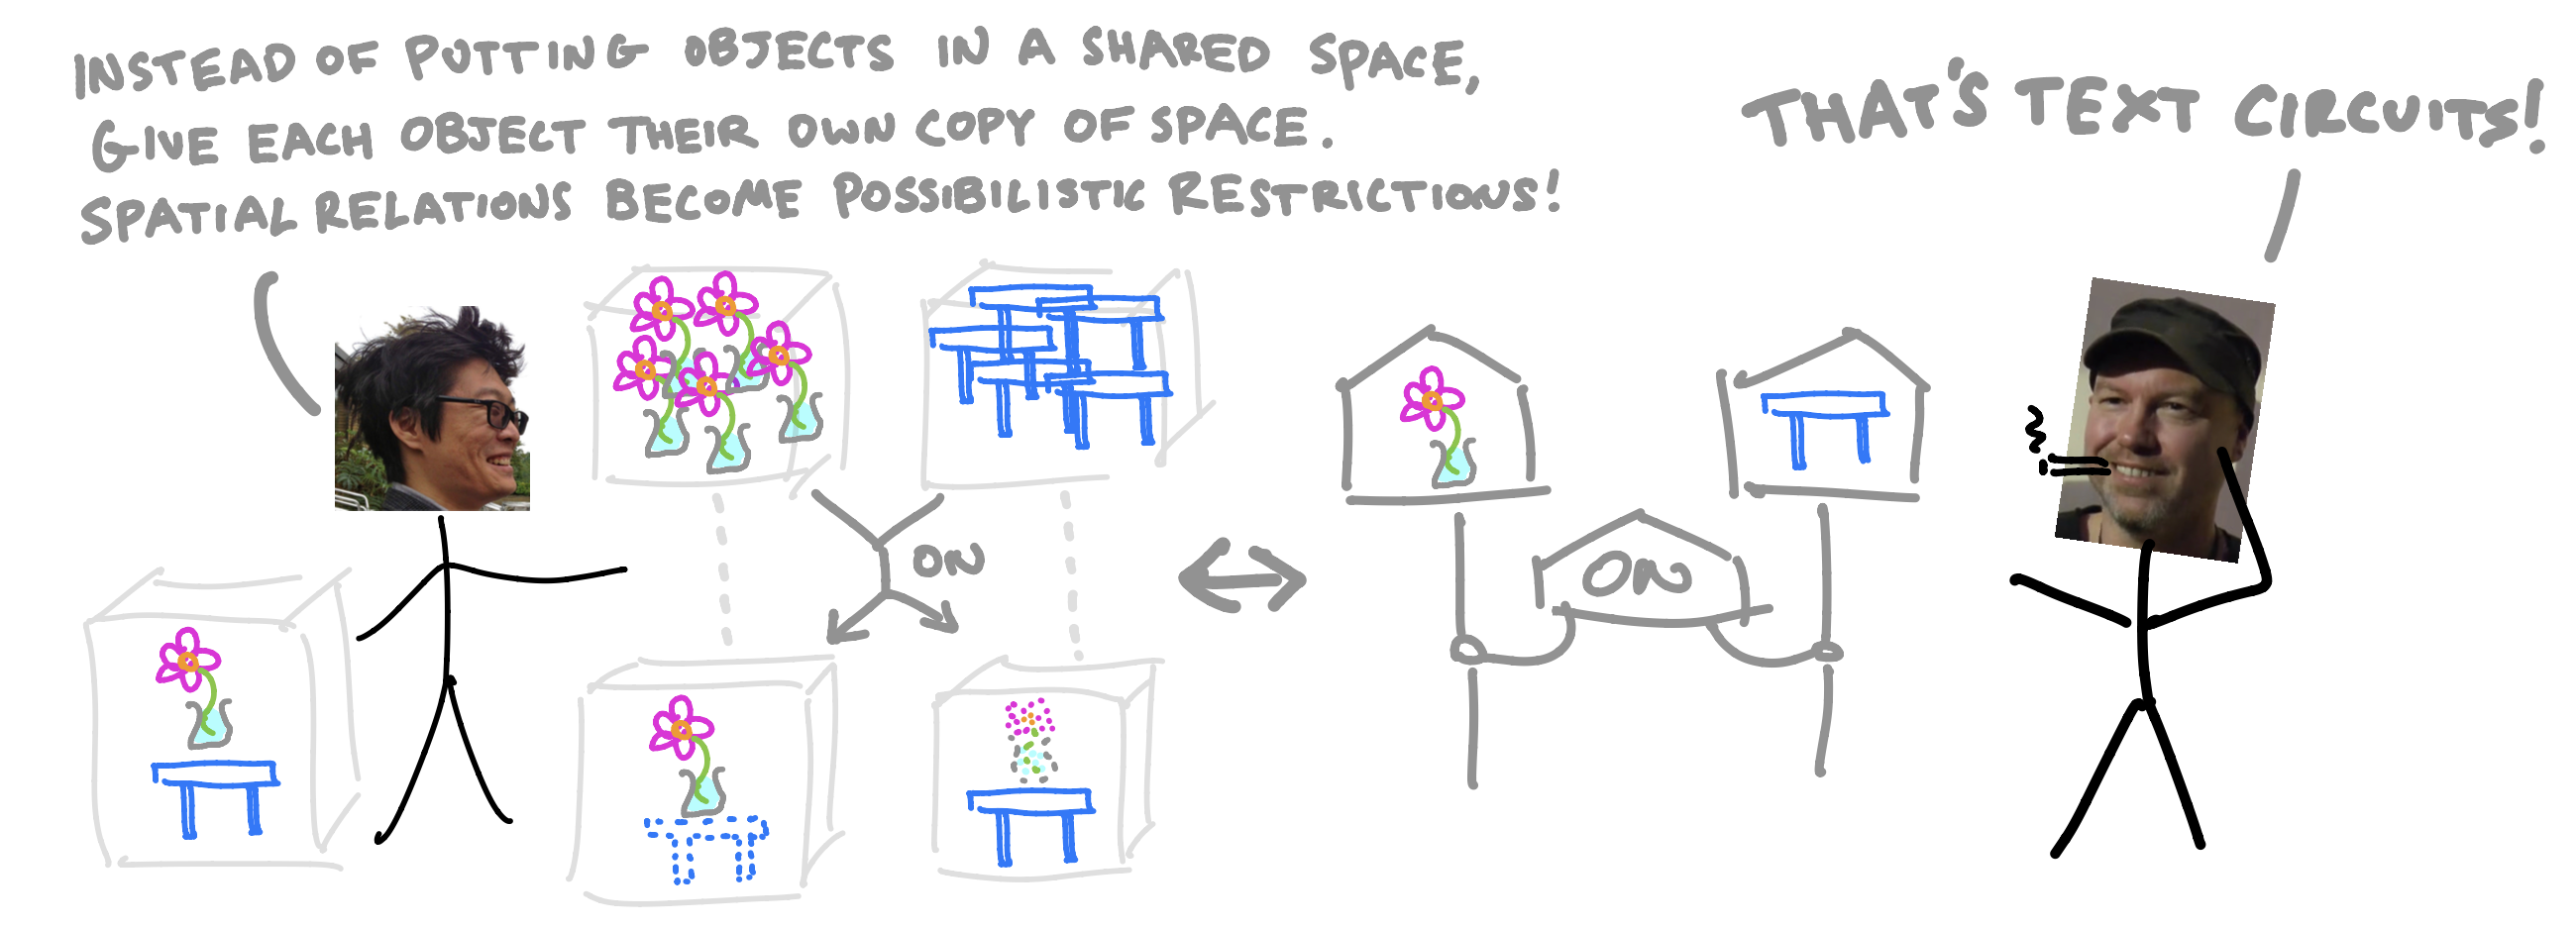
\includegraphics{figures/cartoons/circify1}}
\caption{Then COVID happened. During the first lockdown, I visited Bob's garden under technically legal circumstances, and I suggested a solution to the longstanding problem of representing linguistic spatial relationships. My theoretical concern was the culprit: the initial attempts at the problem failed because the approach was to find a single sentence object $s$ in which one could paste the data of arbitrarily many distinct spatial entities. The simple solution was a change in perspective.}
\end{figure}

\begin{figure}[h!]
\centering
\scalebox{1}{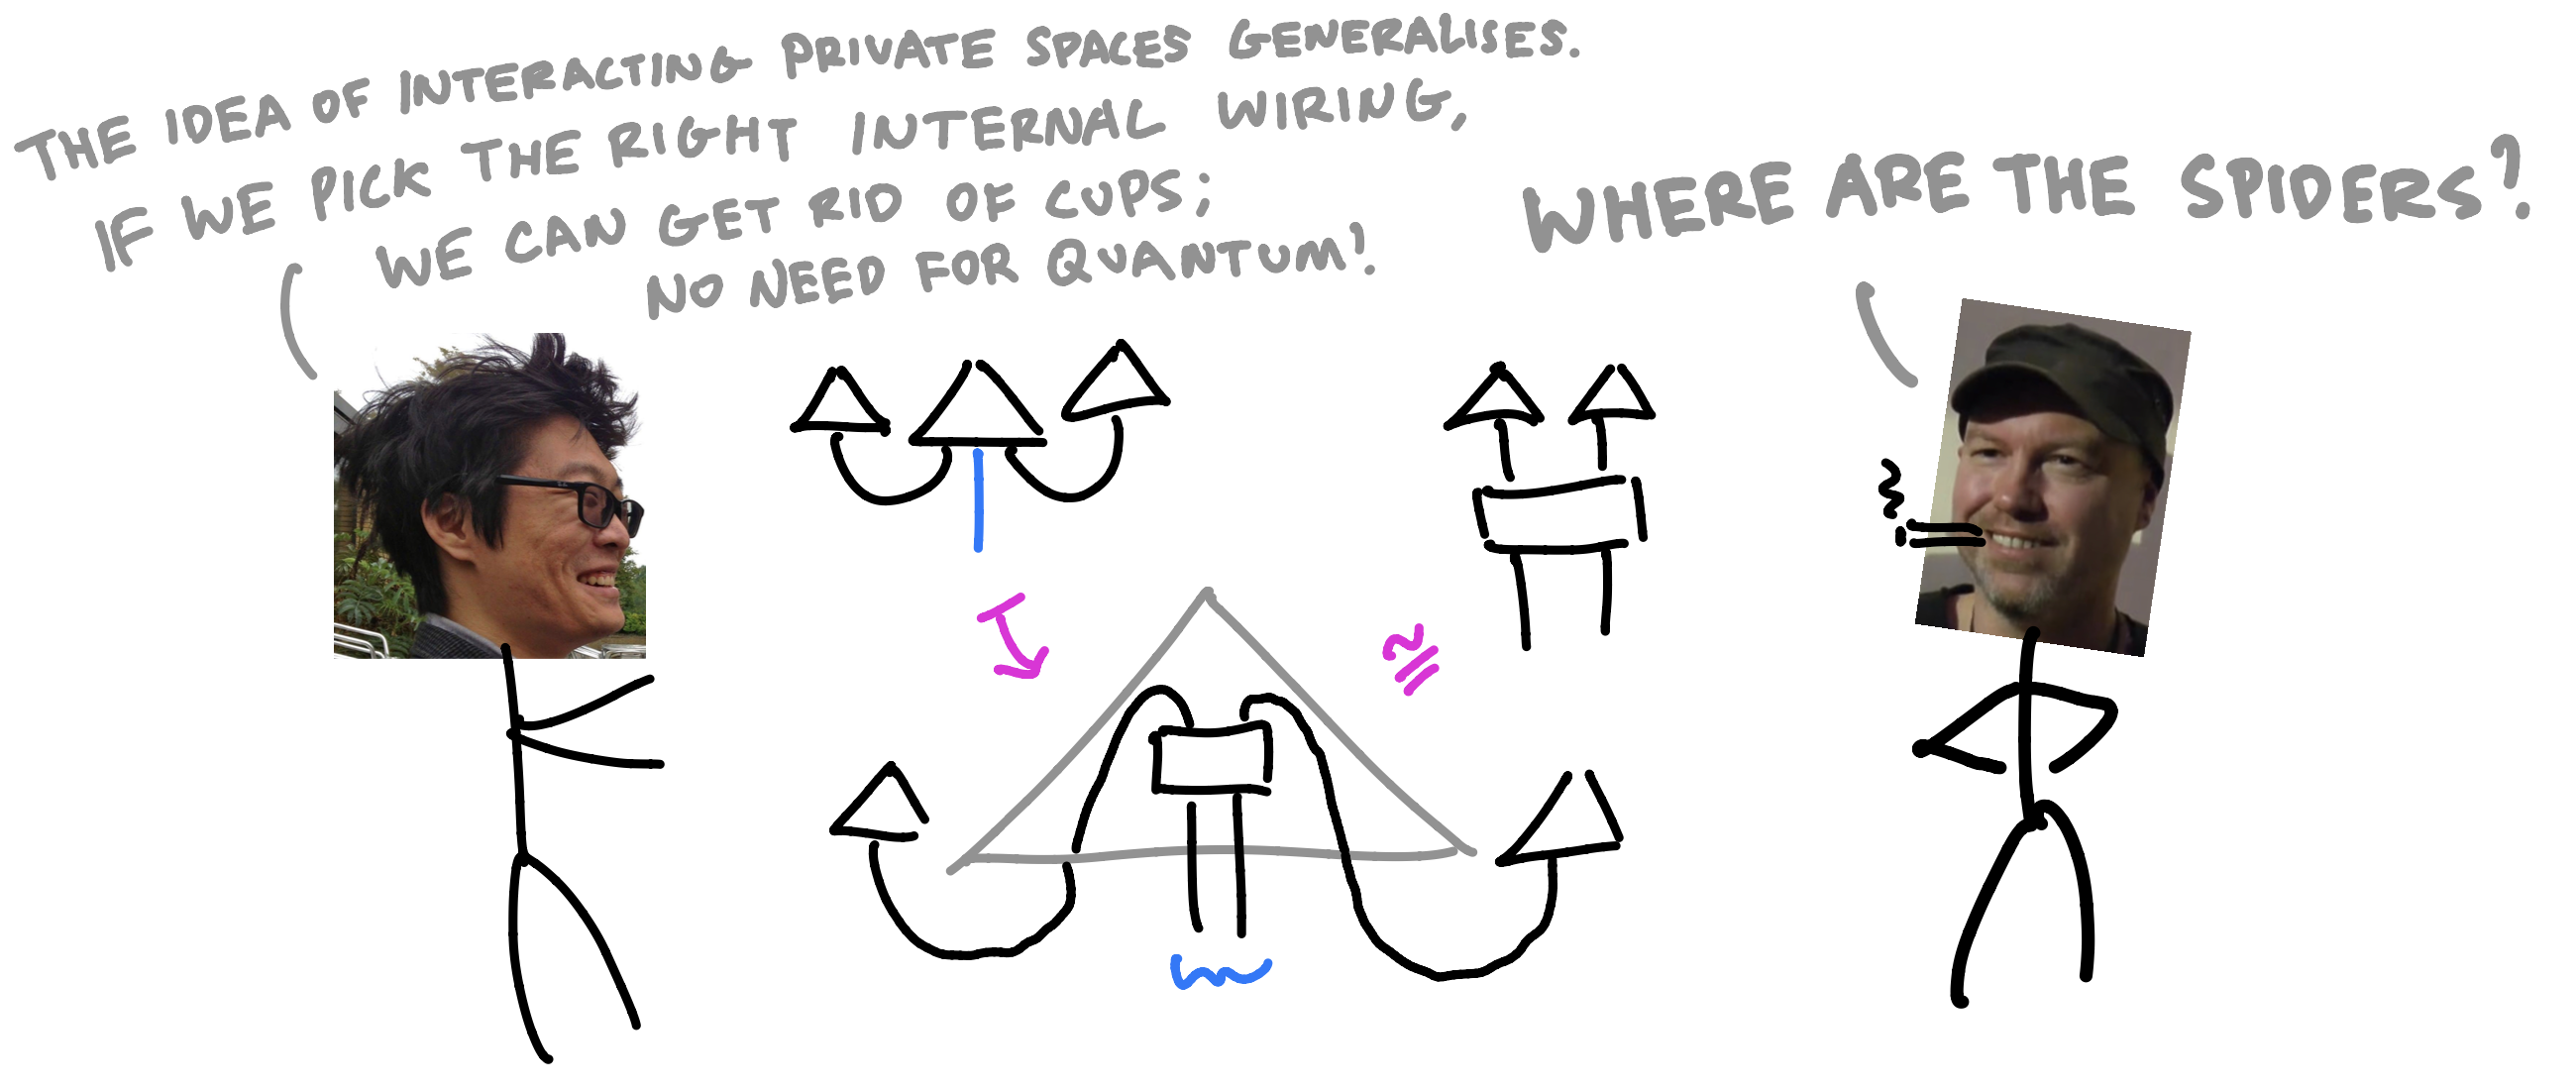
\includegraphics{figures/cartoons/circify2}}
\caption{That this move of splitting up the sentence-wire into a sentence-dependent collection of wires was sufficient to solve what had appeared to be a difficult problem prompted some re-examination of foundations. The free autonomisation trick in conjunction with sentence-wire-as-tensored-nouns seemed promising, but it became clear that right way to drown a DisCoCat thoroughly was to explain and eliminate the spiders.}
\end{figure}

\begin{figure}[h!]
\centering
\scalebox{1}{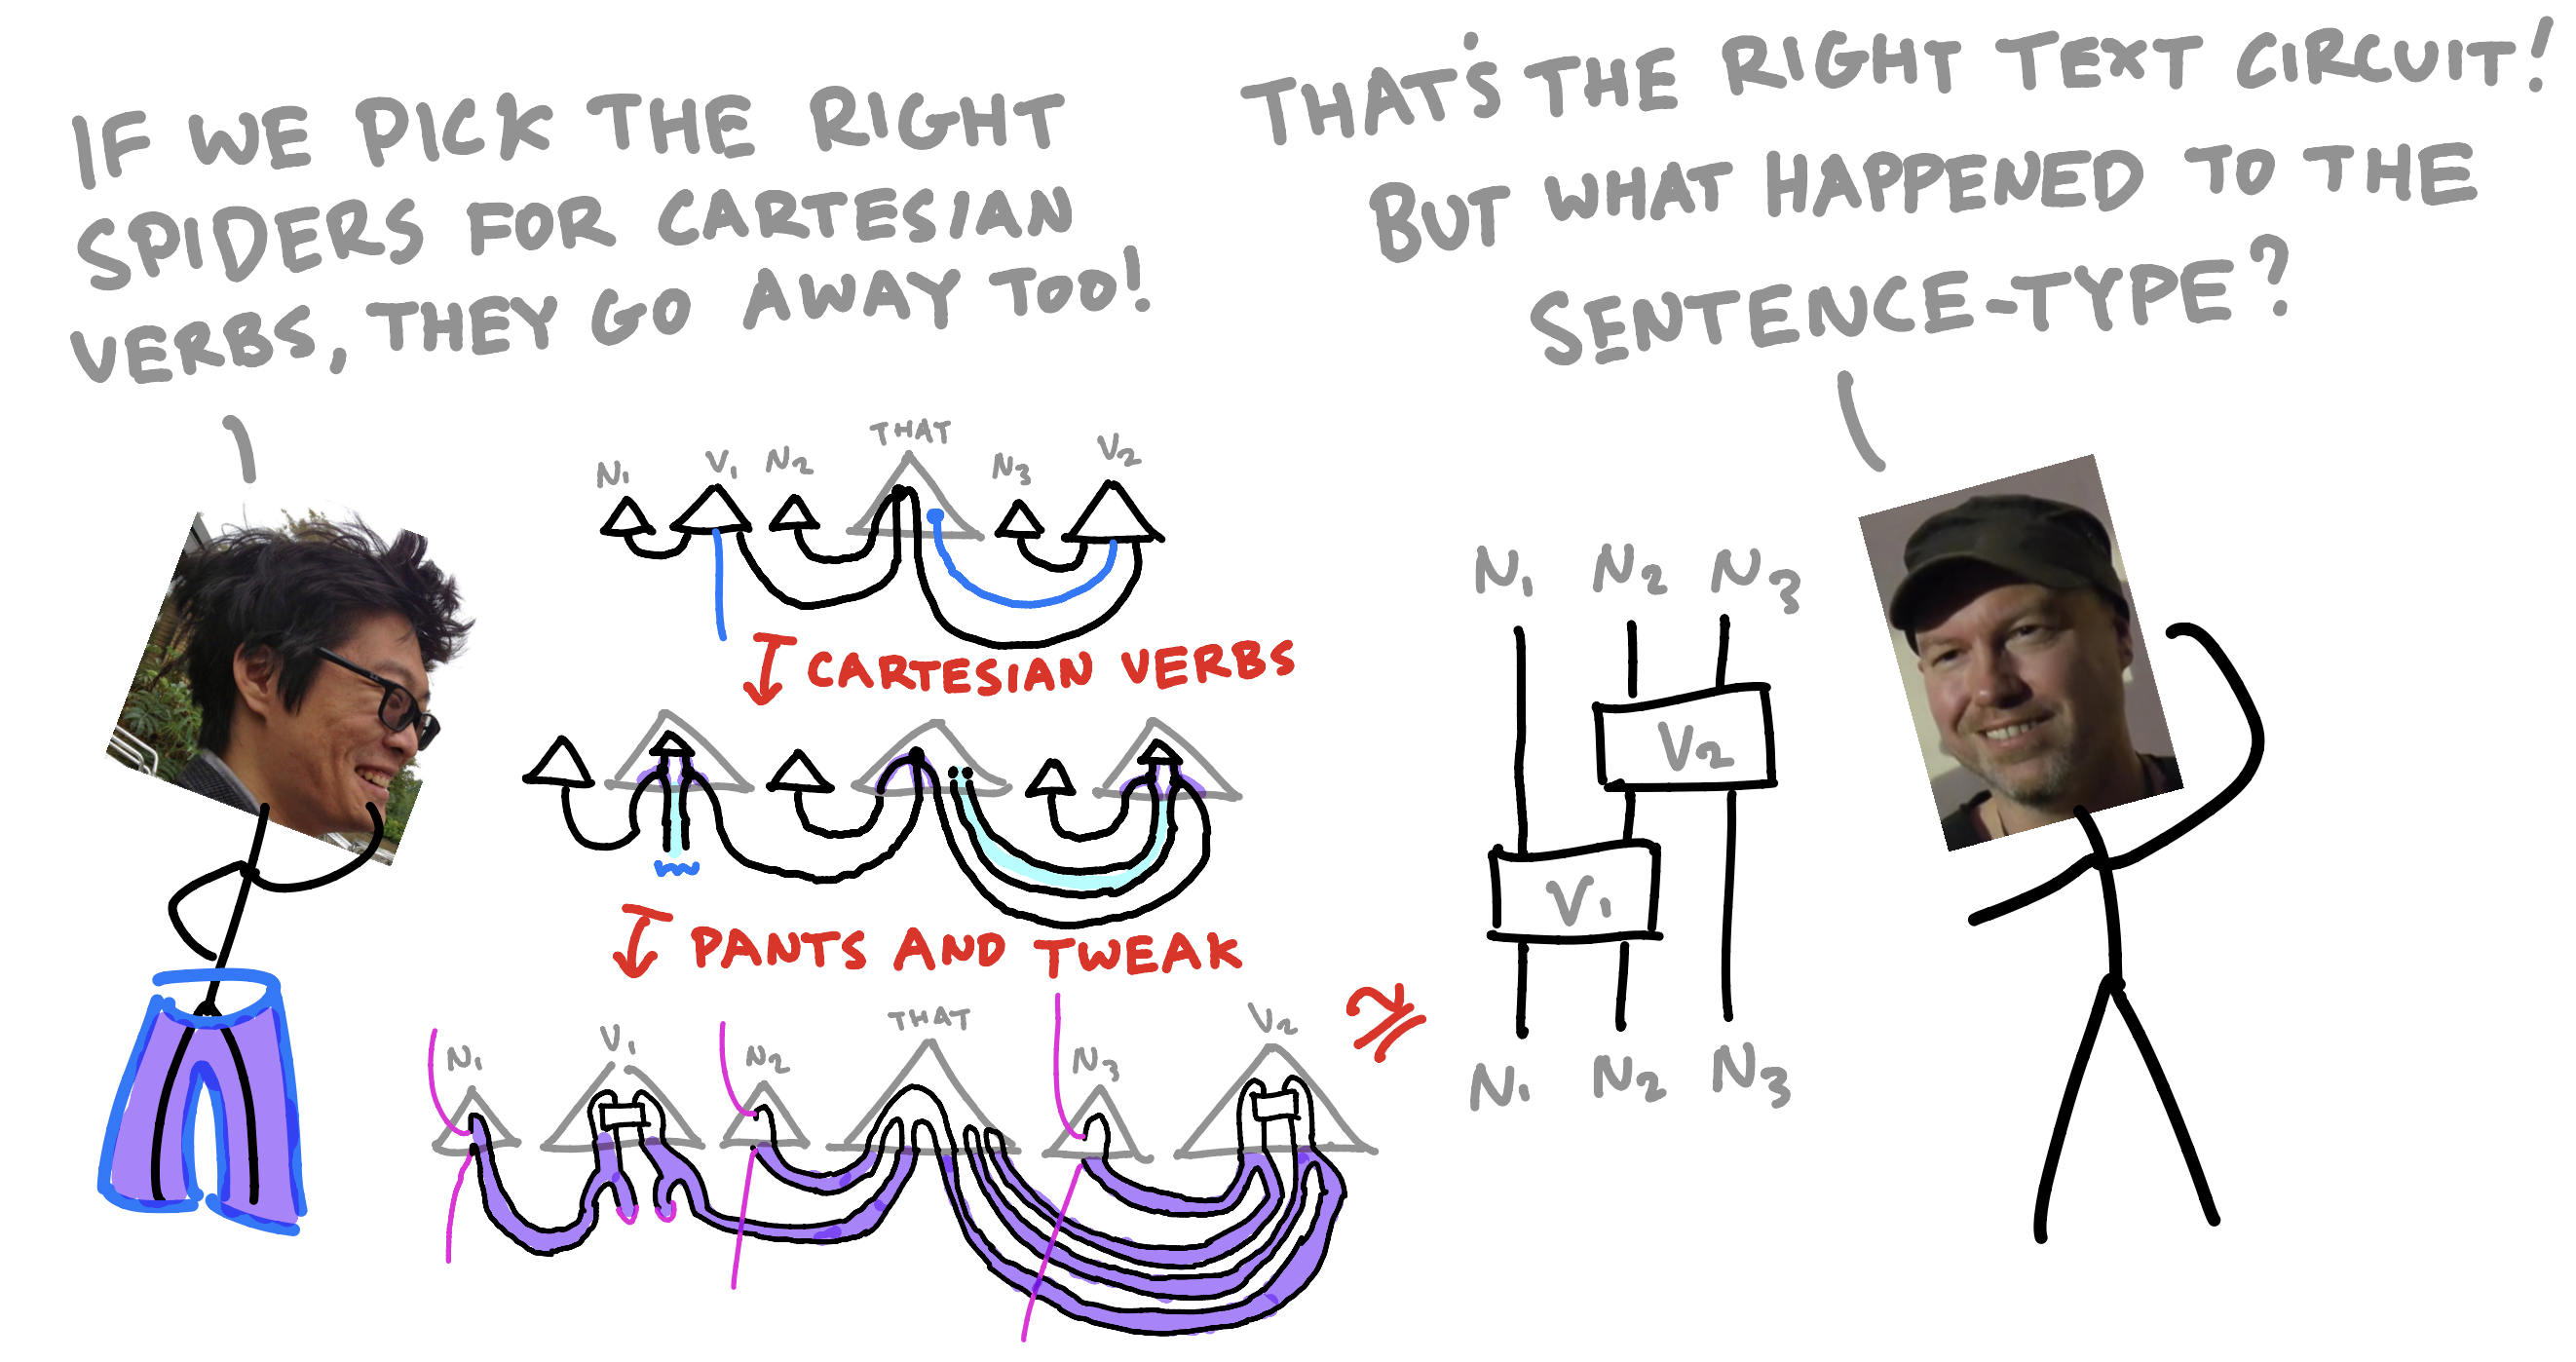
\includegraphics{figures/cartoons/circify3}}
\caption{I then discovered that by interpreting spiders as the well-known "pair of pants" algebra in a compact closed monoidal setting allowed for a procedure in which the final form was purely symmetric monoidal -- the absence of cups and caps meant that there was no practical necessity to interpret diagrams on quantum computers: \emph{any} computer would suffice. The role of spiders for relative pronouns was illuminated in the presence of splitting the sentence wire: the pair-of-pants are the algebra of morphism composition, and splitting the sentence wire into a collection of nouns allowed relative-pronoun-spiders to pick out the participating nouns to compose relationships onto.}
\end{figure}

\begin{figure}[h!]
\centering
\scalebox{1}{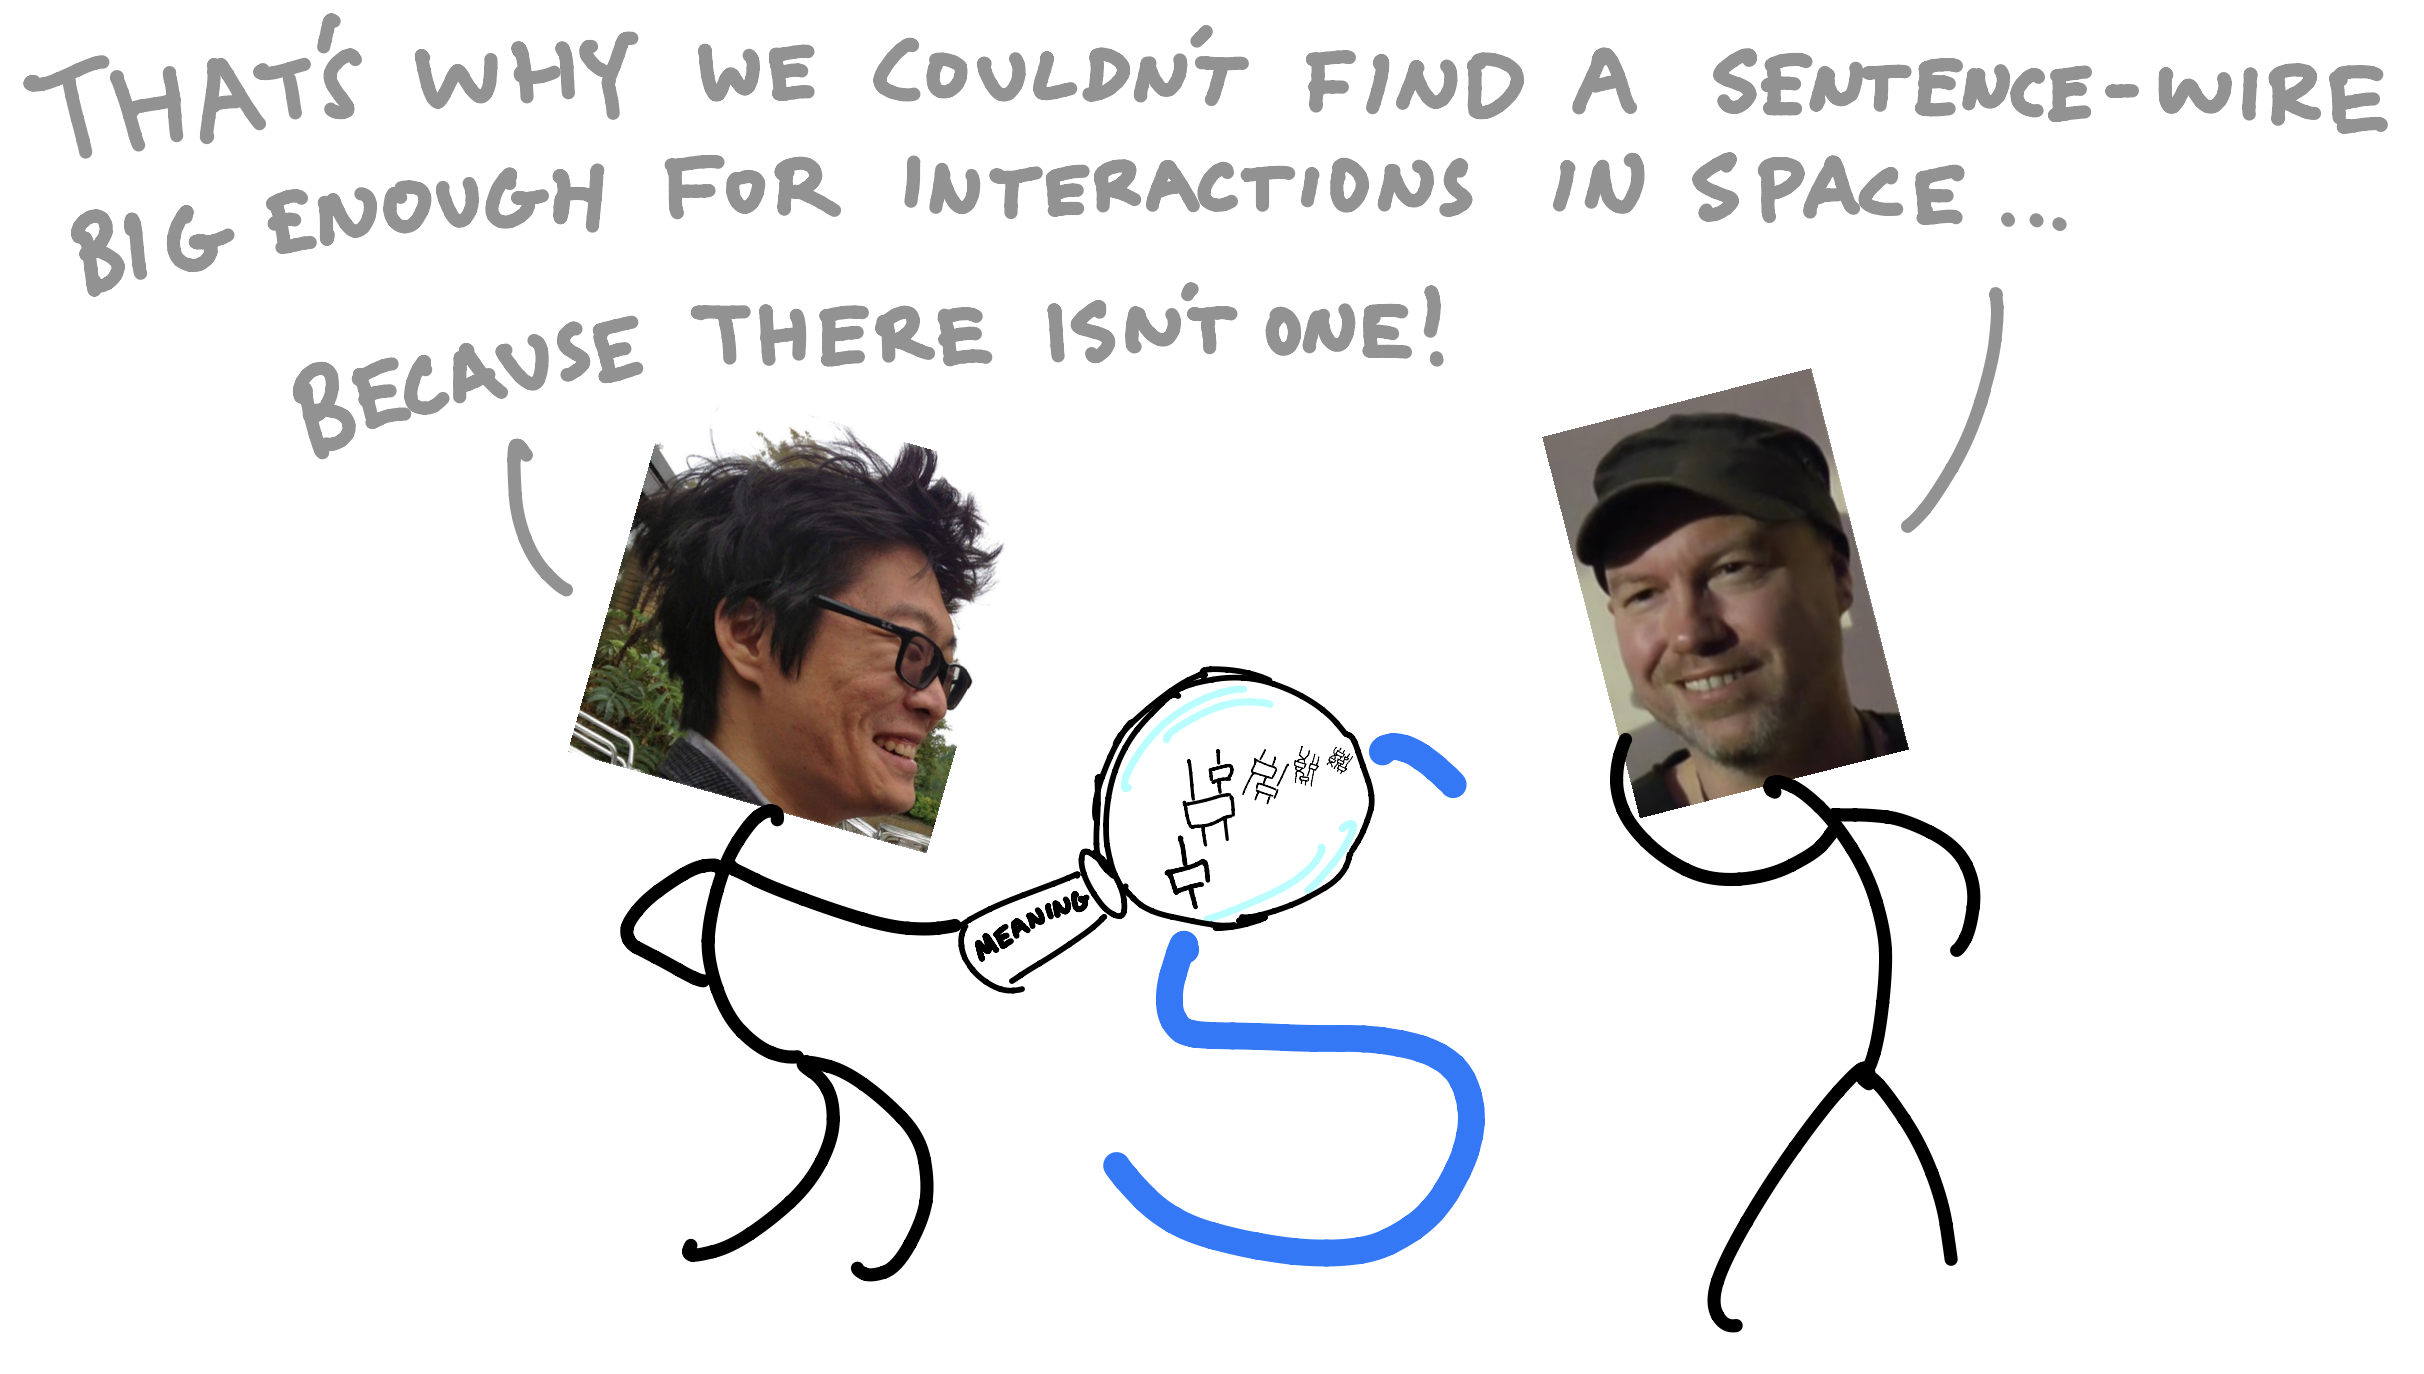
\includegraphics{figures/cartoons/nosent}}
\caption{A coherent conservative generalisation of DisCoCat with less baggage had emerged, or rather, DisCoCirc was placed to formally subsume DisCoCat. It was now understood that the sentence type was a formal syntactic ansatz for the sake of grammar, which was to be interpreted in the semantic domain not as a single wire, but as a sentence-dependent collection of wires. It was further realised that the complexity of pregroup diagrams was due to grammar -- the topological deformation of semantic connections to fit the one-dimensional line of language -- whereas the essential connective content of language could be expressed in a simple form that distilled away the bureaucracy of syntax.}
\end{figure}

\begin{figure}[h!]
\centering
\scalebox{1}{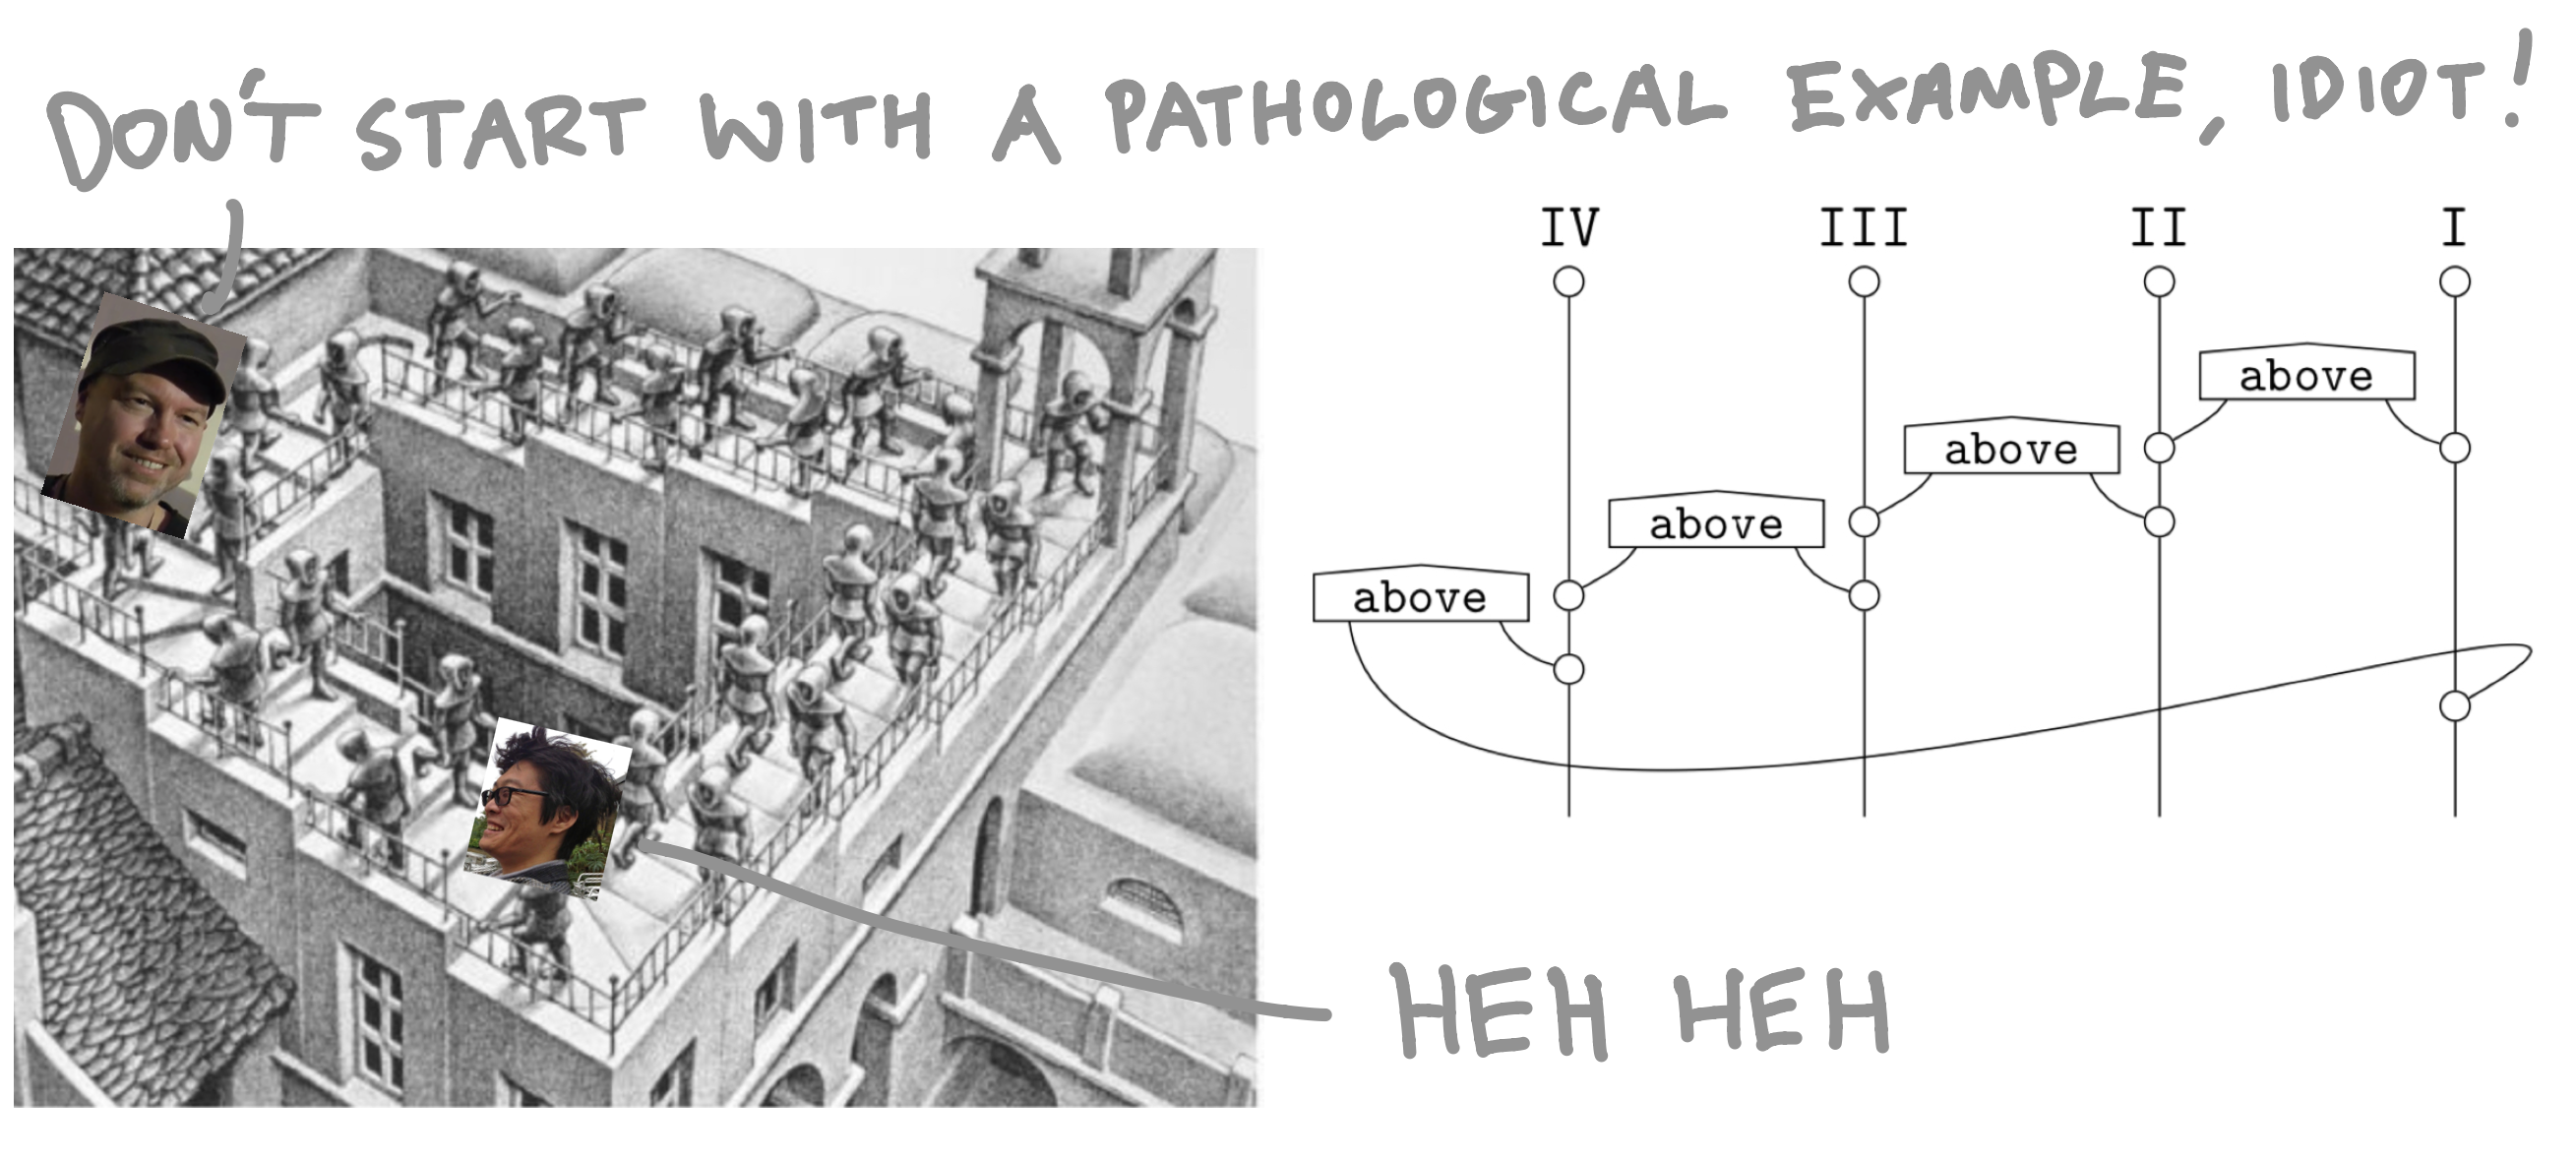
\includegraphics{figures/cartoons/space1}}
\caption{We wrote up the story about spaces in \bR CITE \e, the spiritual successor to \emph{interacting conceptual spaces I}. We could formally calculate the meanings of sentences that used linguistic spatial relations, all using a simple and tactile diagrammatic calculus.}
\end{figure}

\begin{figure}[h!]
\centering
\scalebox{1}{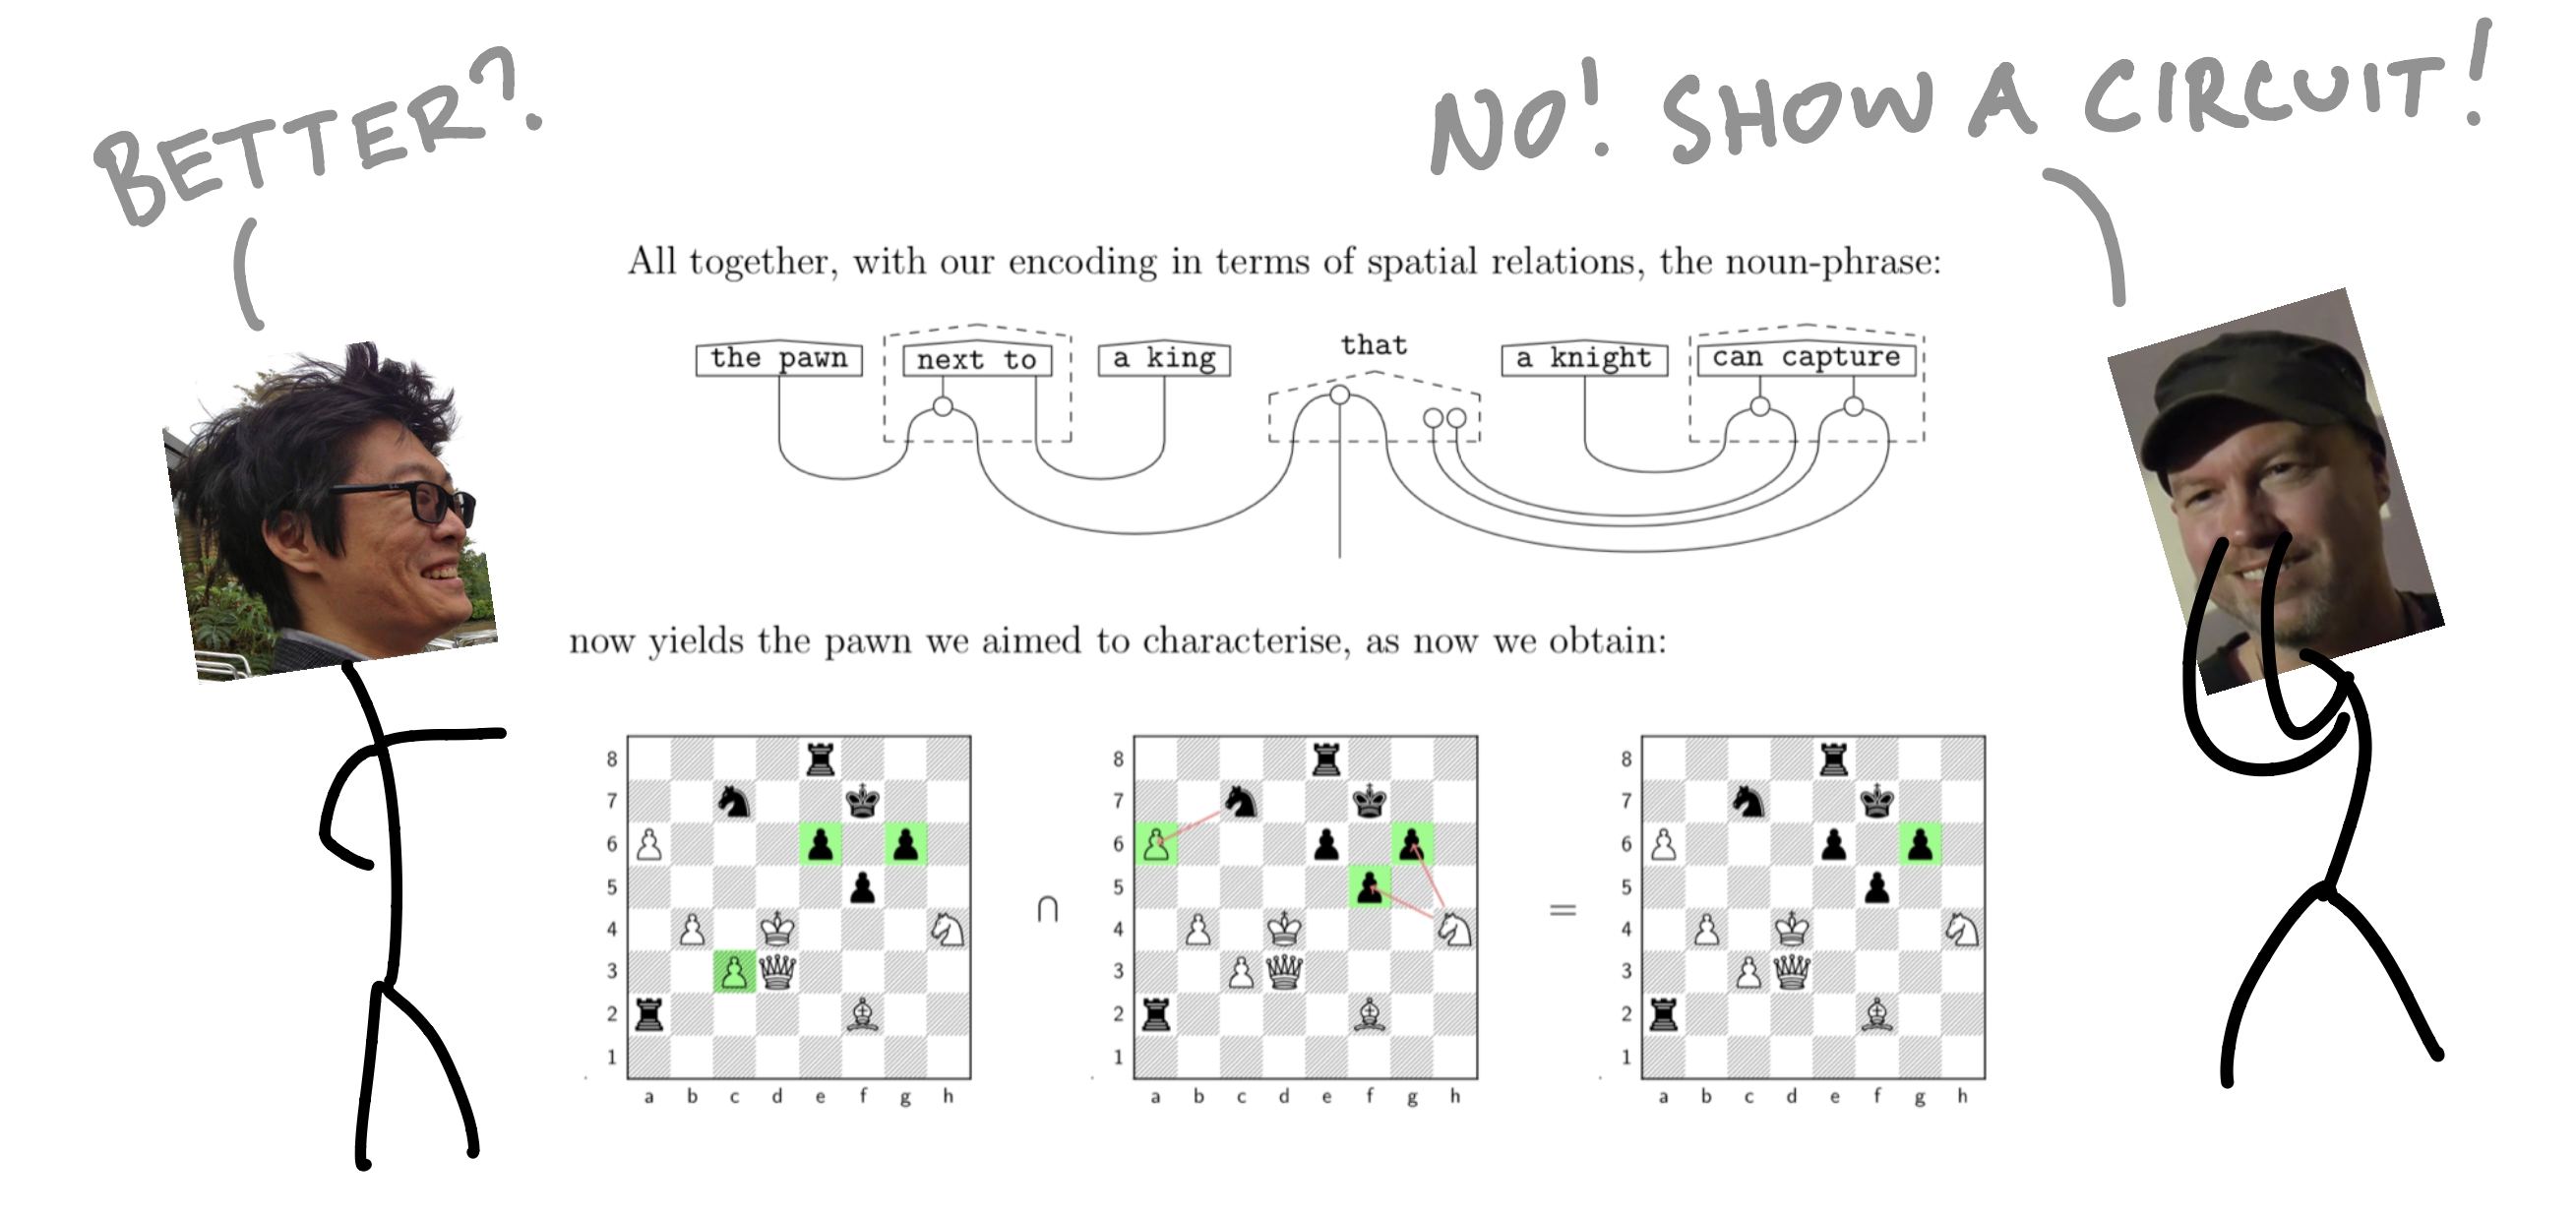
\includegraphics{figures/cartoons/space2}}
\end{figure}

\begin{figure}[h!]
\centering
\scalebox{1}{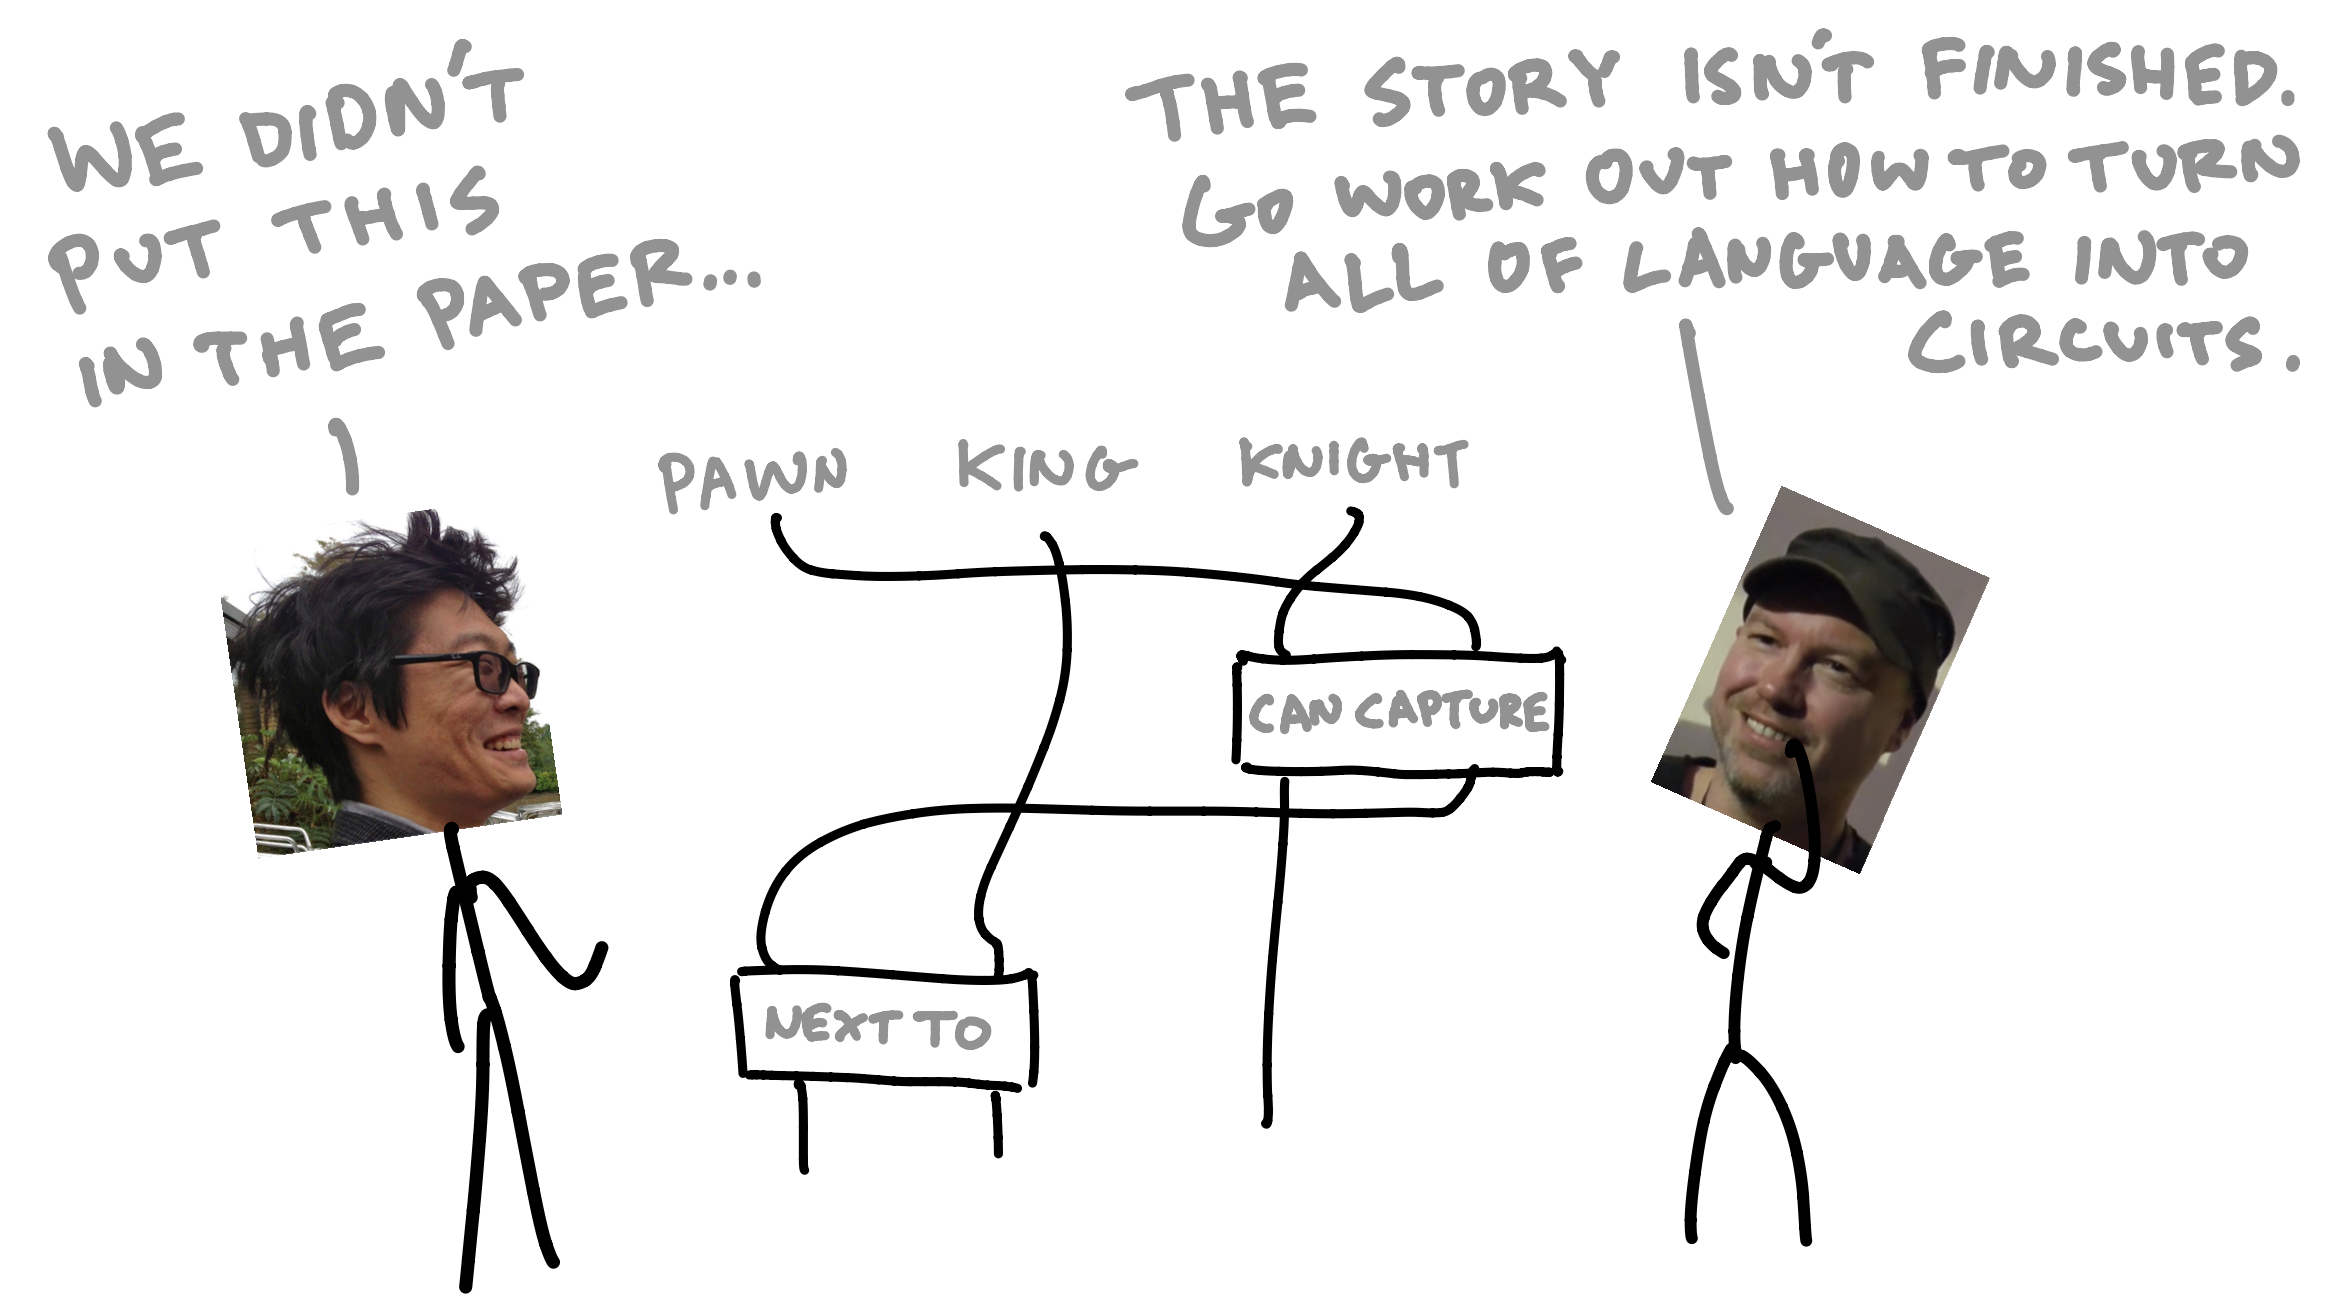
\includegraphics{figures/cartoons/space3}}
\caption{The paper on spatial relations actually came very late, because I was busy with Bob's ludicrous request to go turn "all of language" into circuits. I bitched and moaned about how I wasn't a linguist and how it was an impossible task, but I was in too deep to back out.}
\end{figure}

\begin{figure}[h!]
\centering
\scalebox{1}{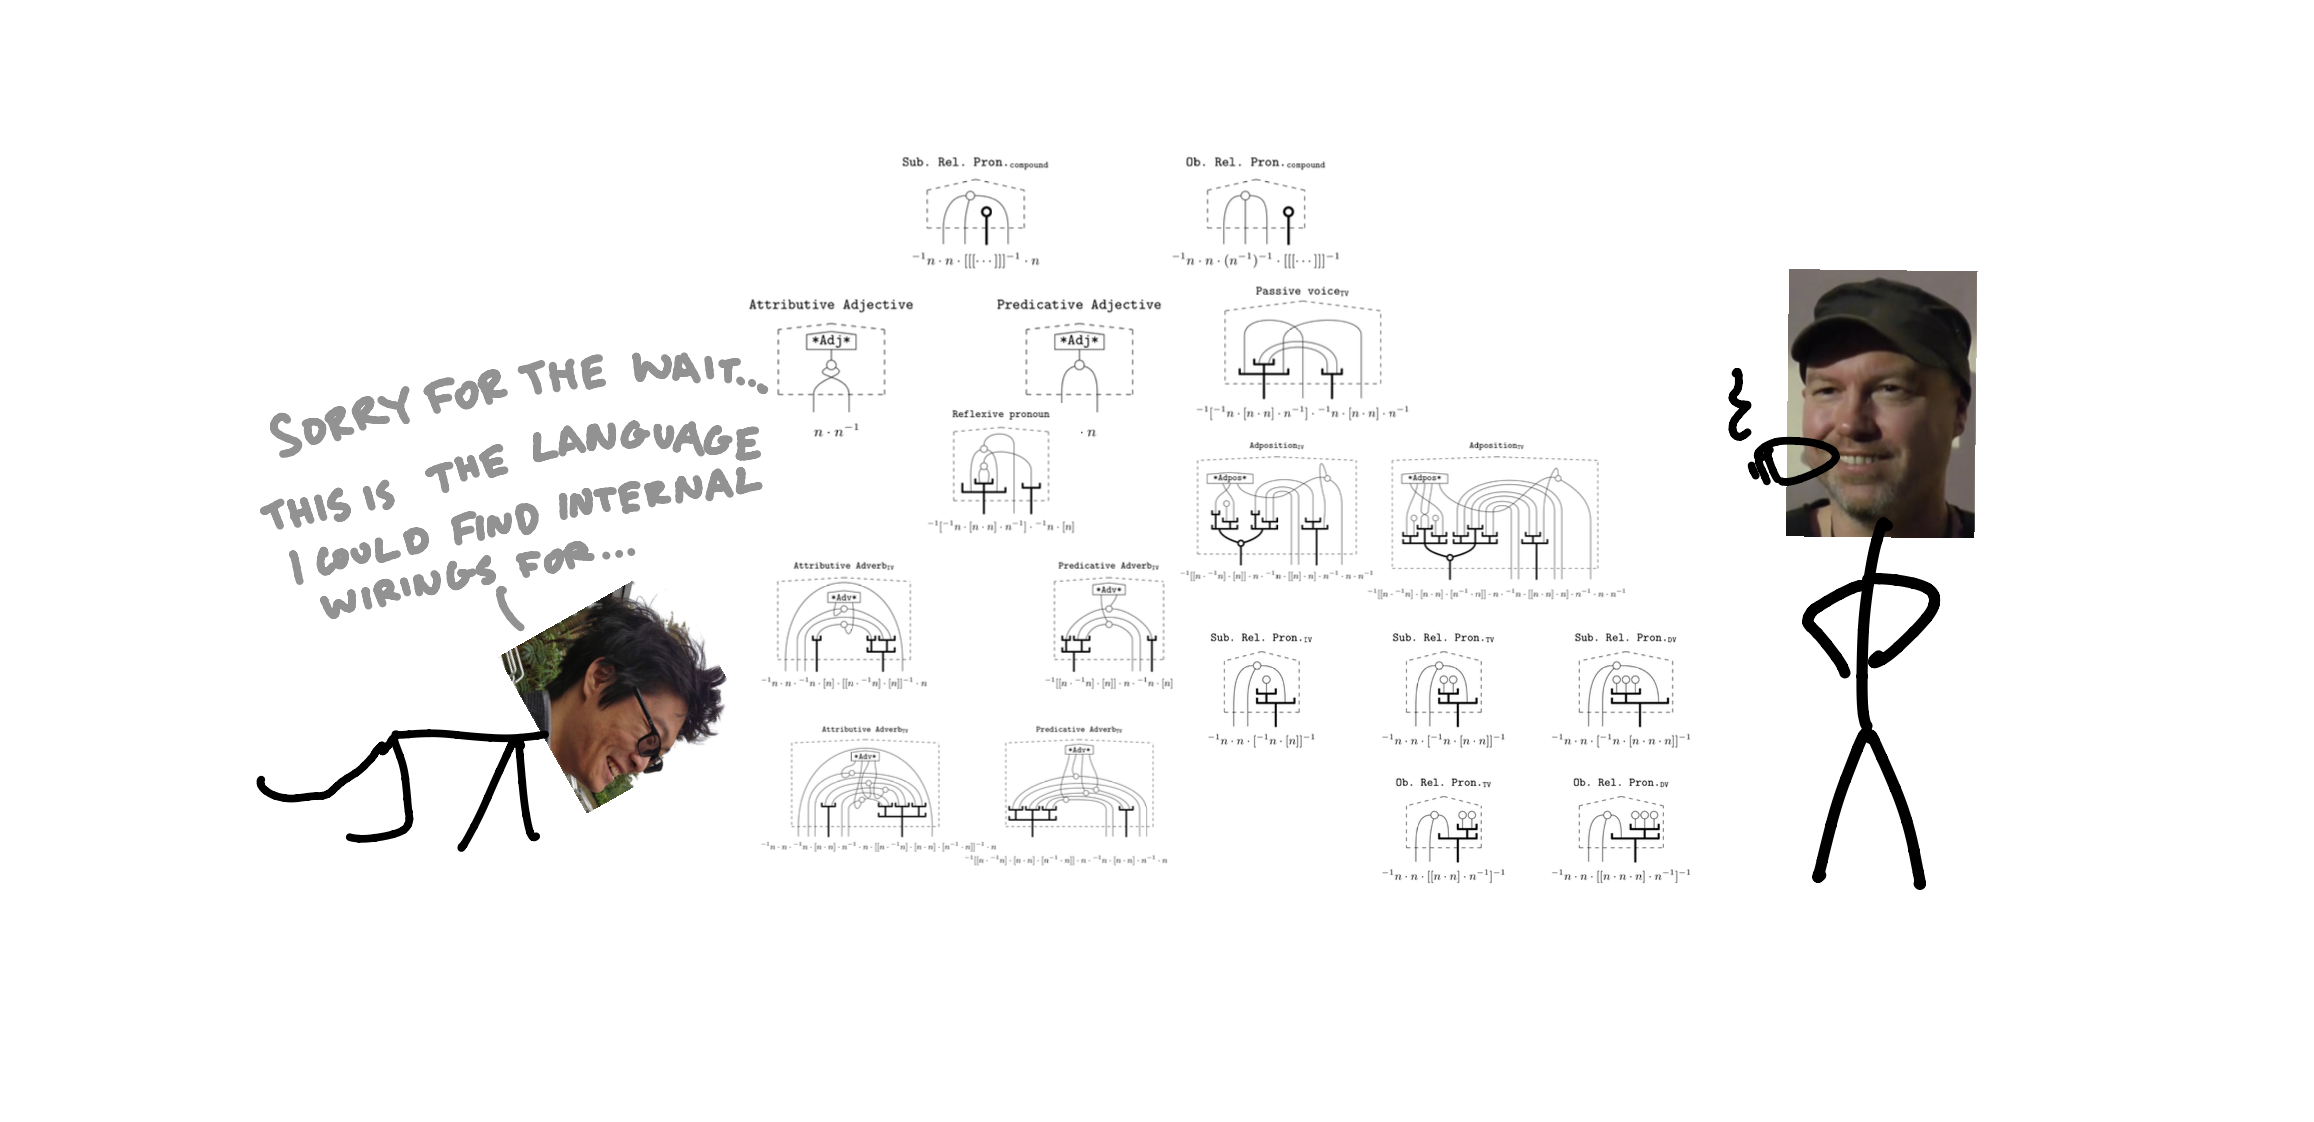
\includegraphics{figures/cartoons/pregroup1}}
\caption{I suppose the nice thing about aiming for the moon is that even failure might mean you leave orbit. So I settled for what I thought was a sensible fragment of English, for which I devised internal wirings and an algorithm that transformed pregroup diagrams with the internal wirings into circuit form. Many tiring diagrams later, I presented my results in the first draft of "distilling text into circuits".}
\end{figure}

\begin{figure}[h!]
\centering
\scalebox{1}{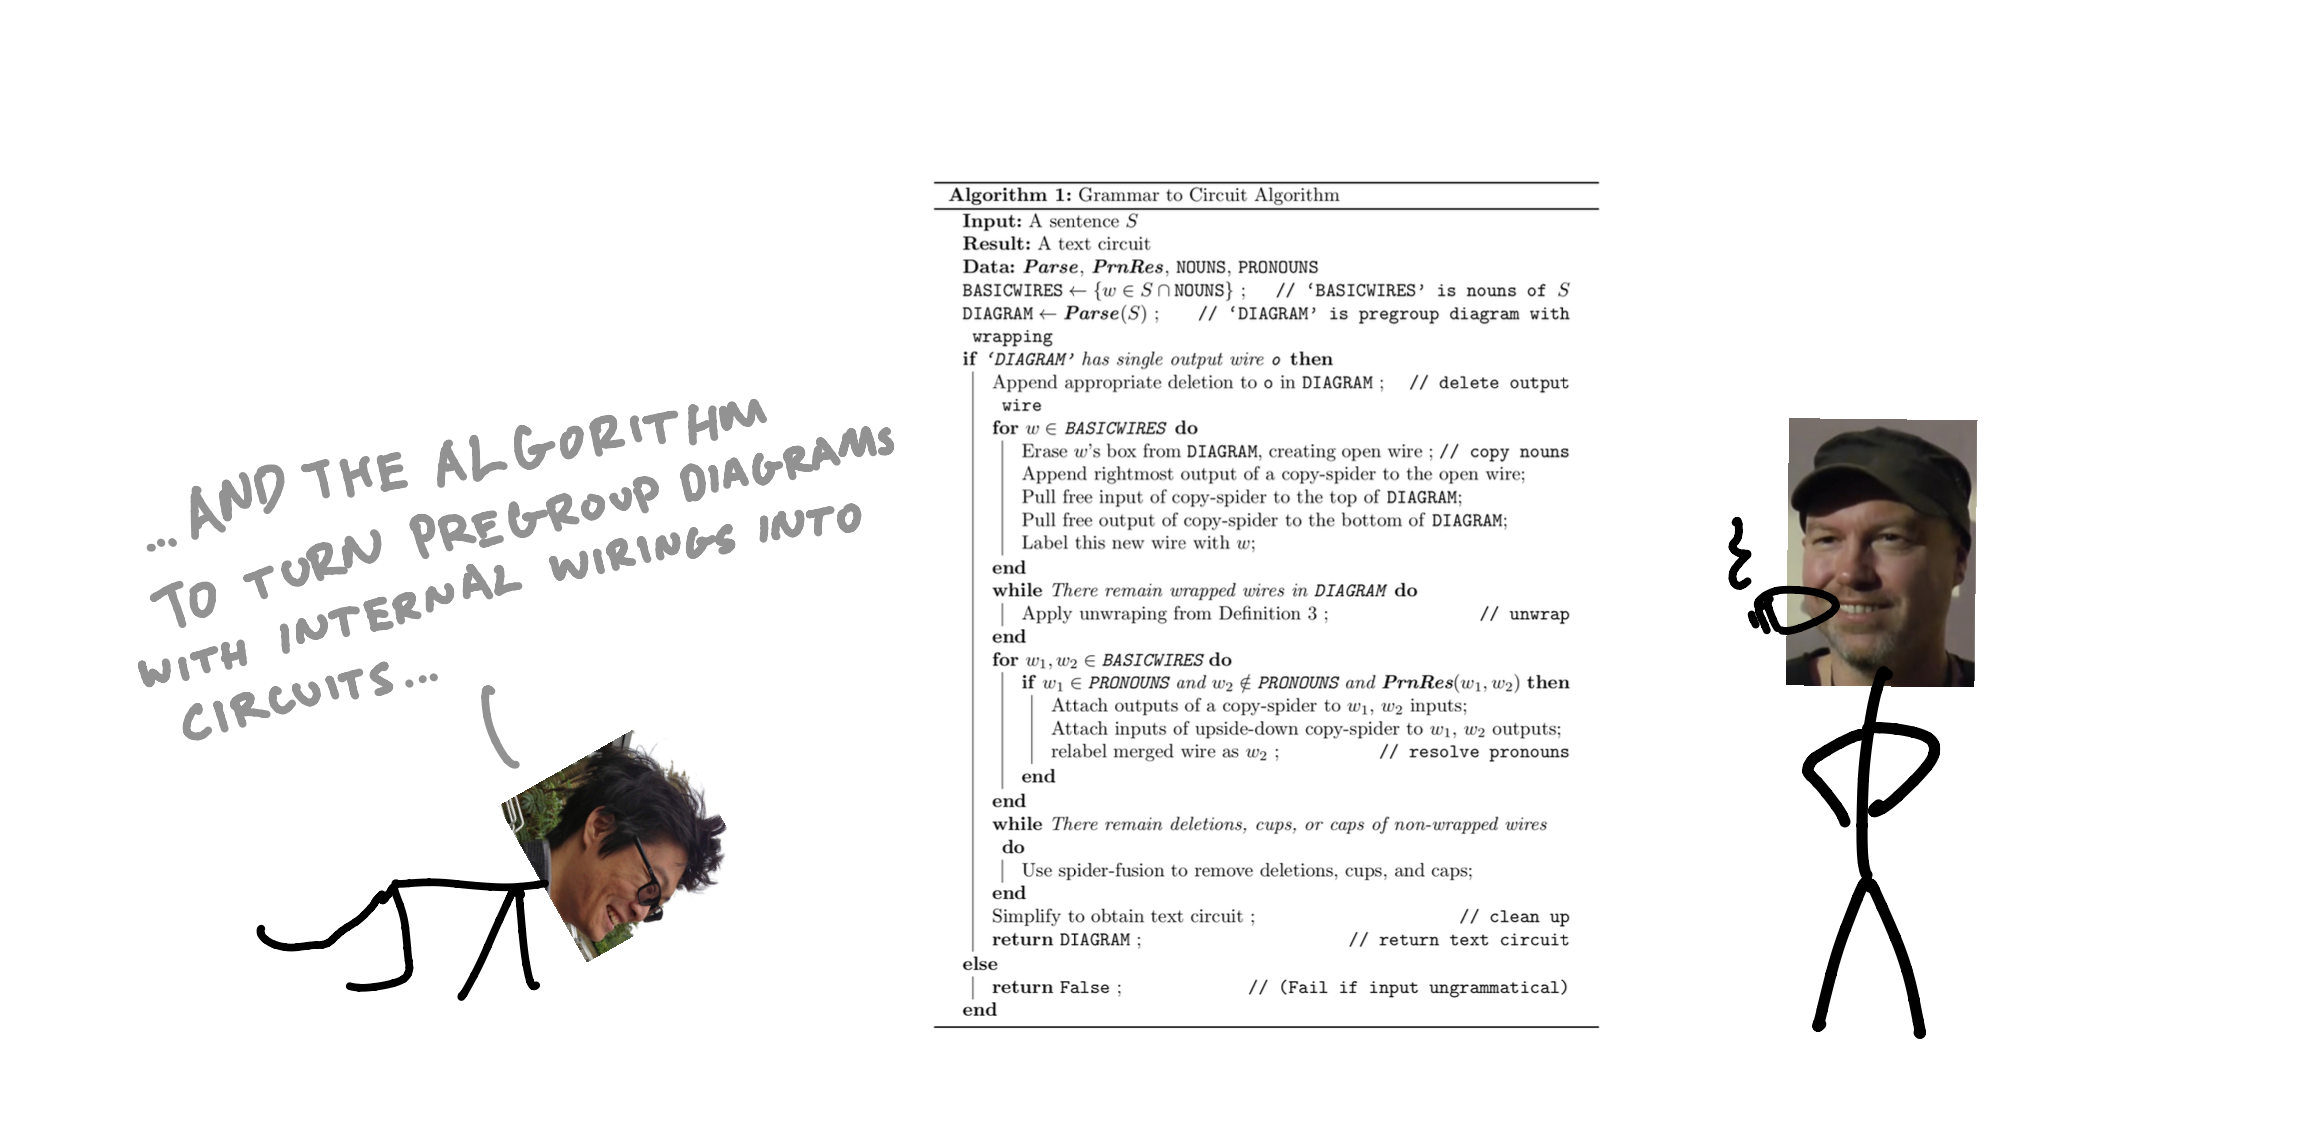
\includegraphics{figures/cartoons/pregroup2}}
\end{figure}

\begin{figure}[h!]
\centering
\scalebox{1}{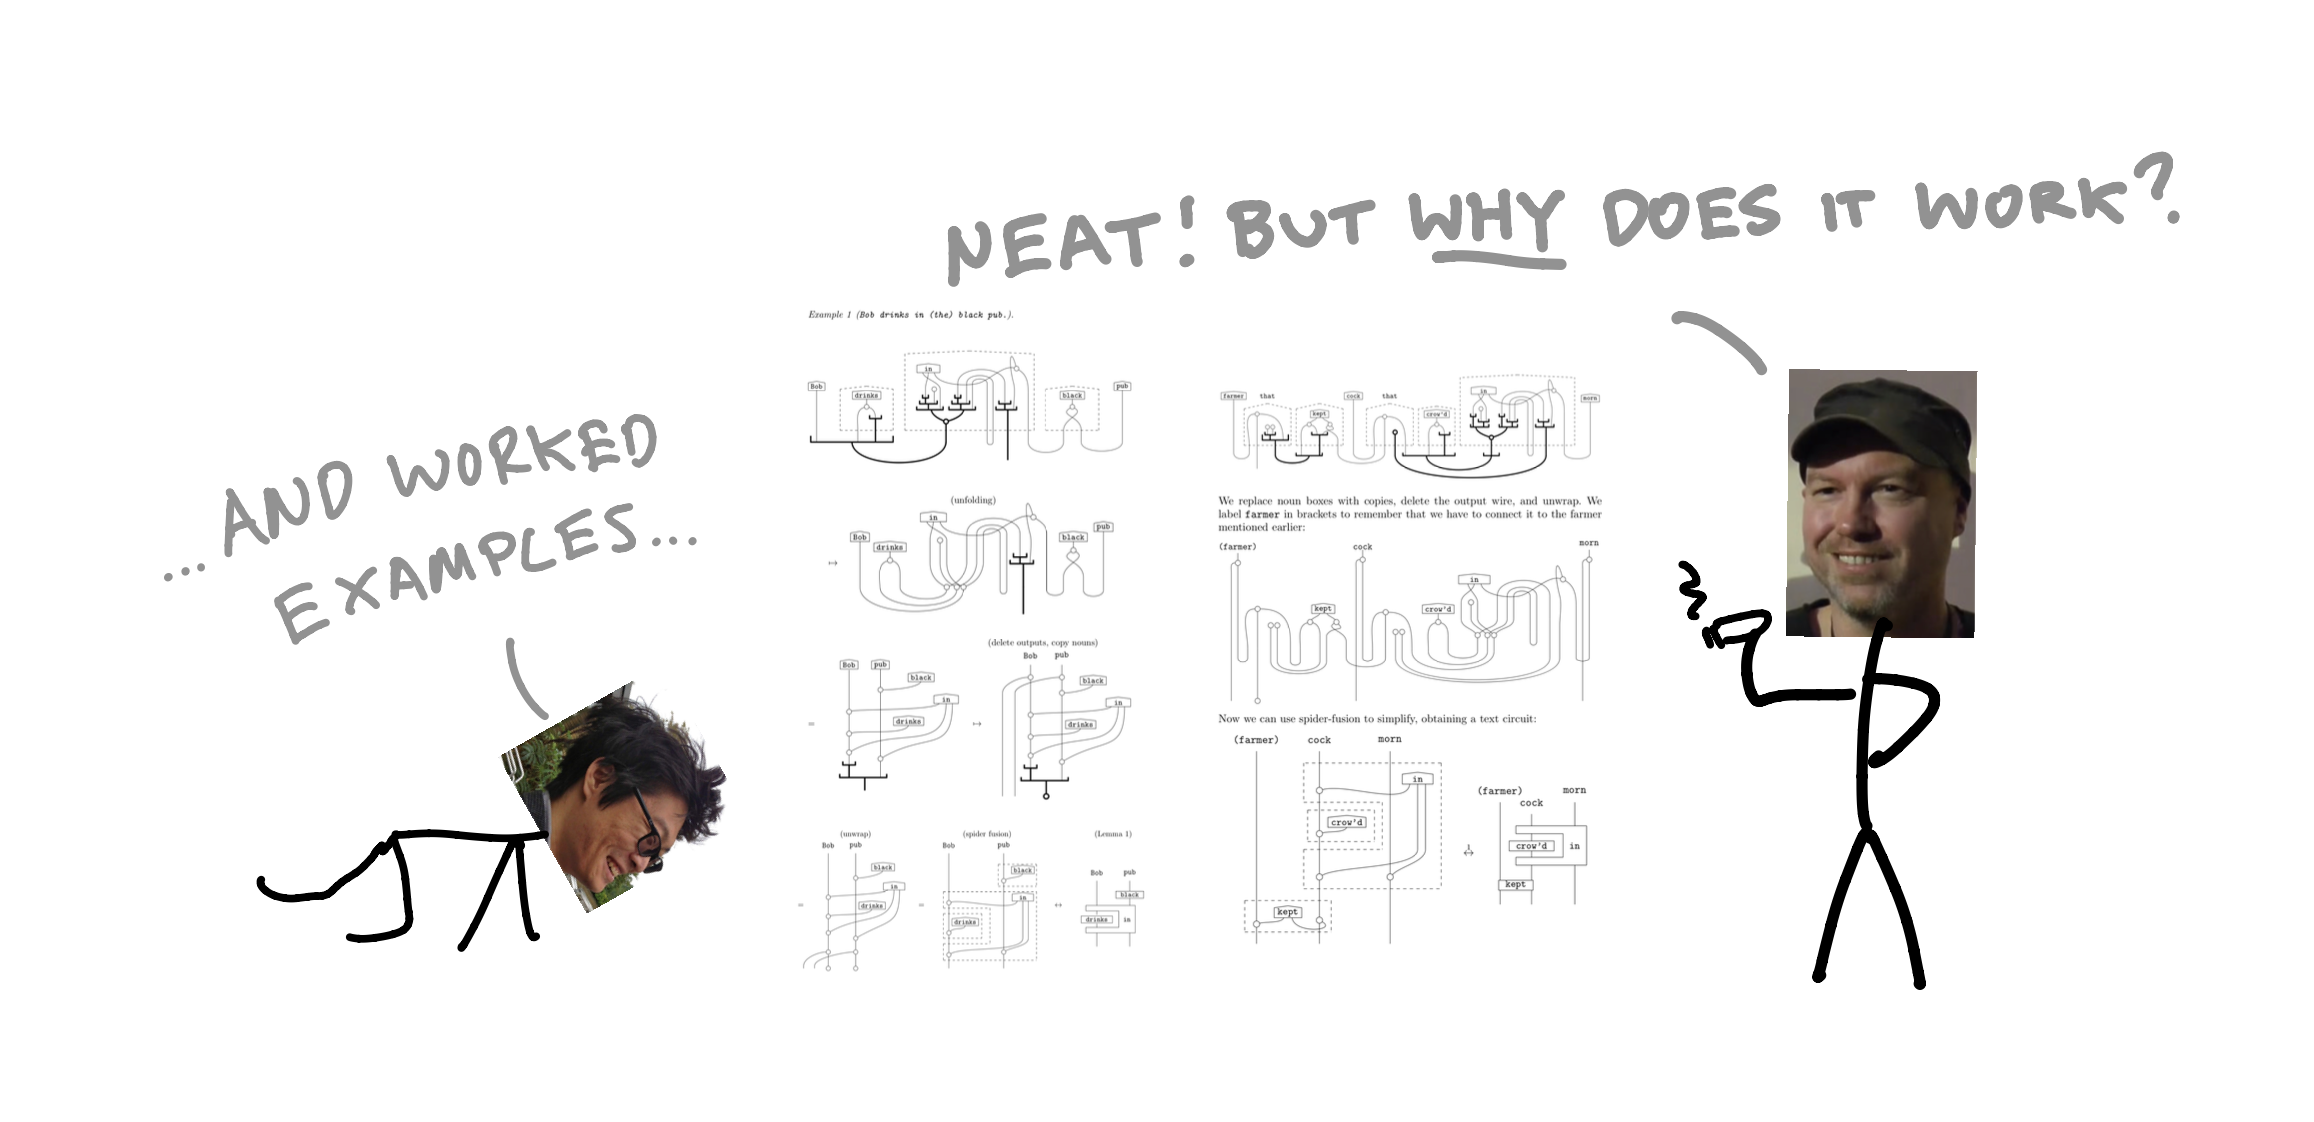
\includegraphics{figures/cartoons/pregroup3}}
\end{figure}

\begin{figure}[h!]
\centering
\scalebox{1}{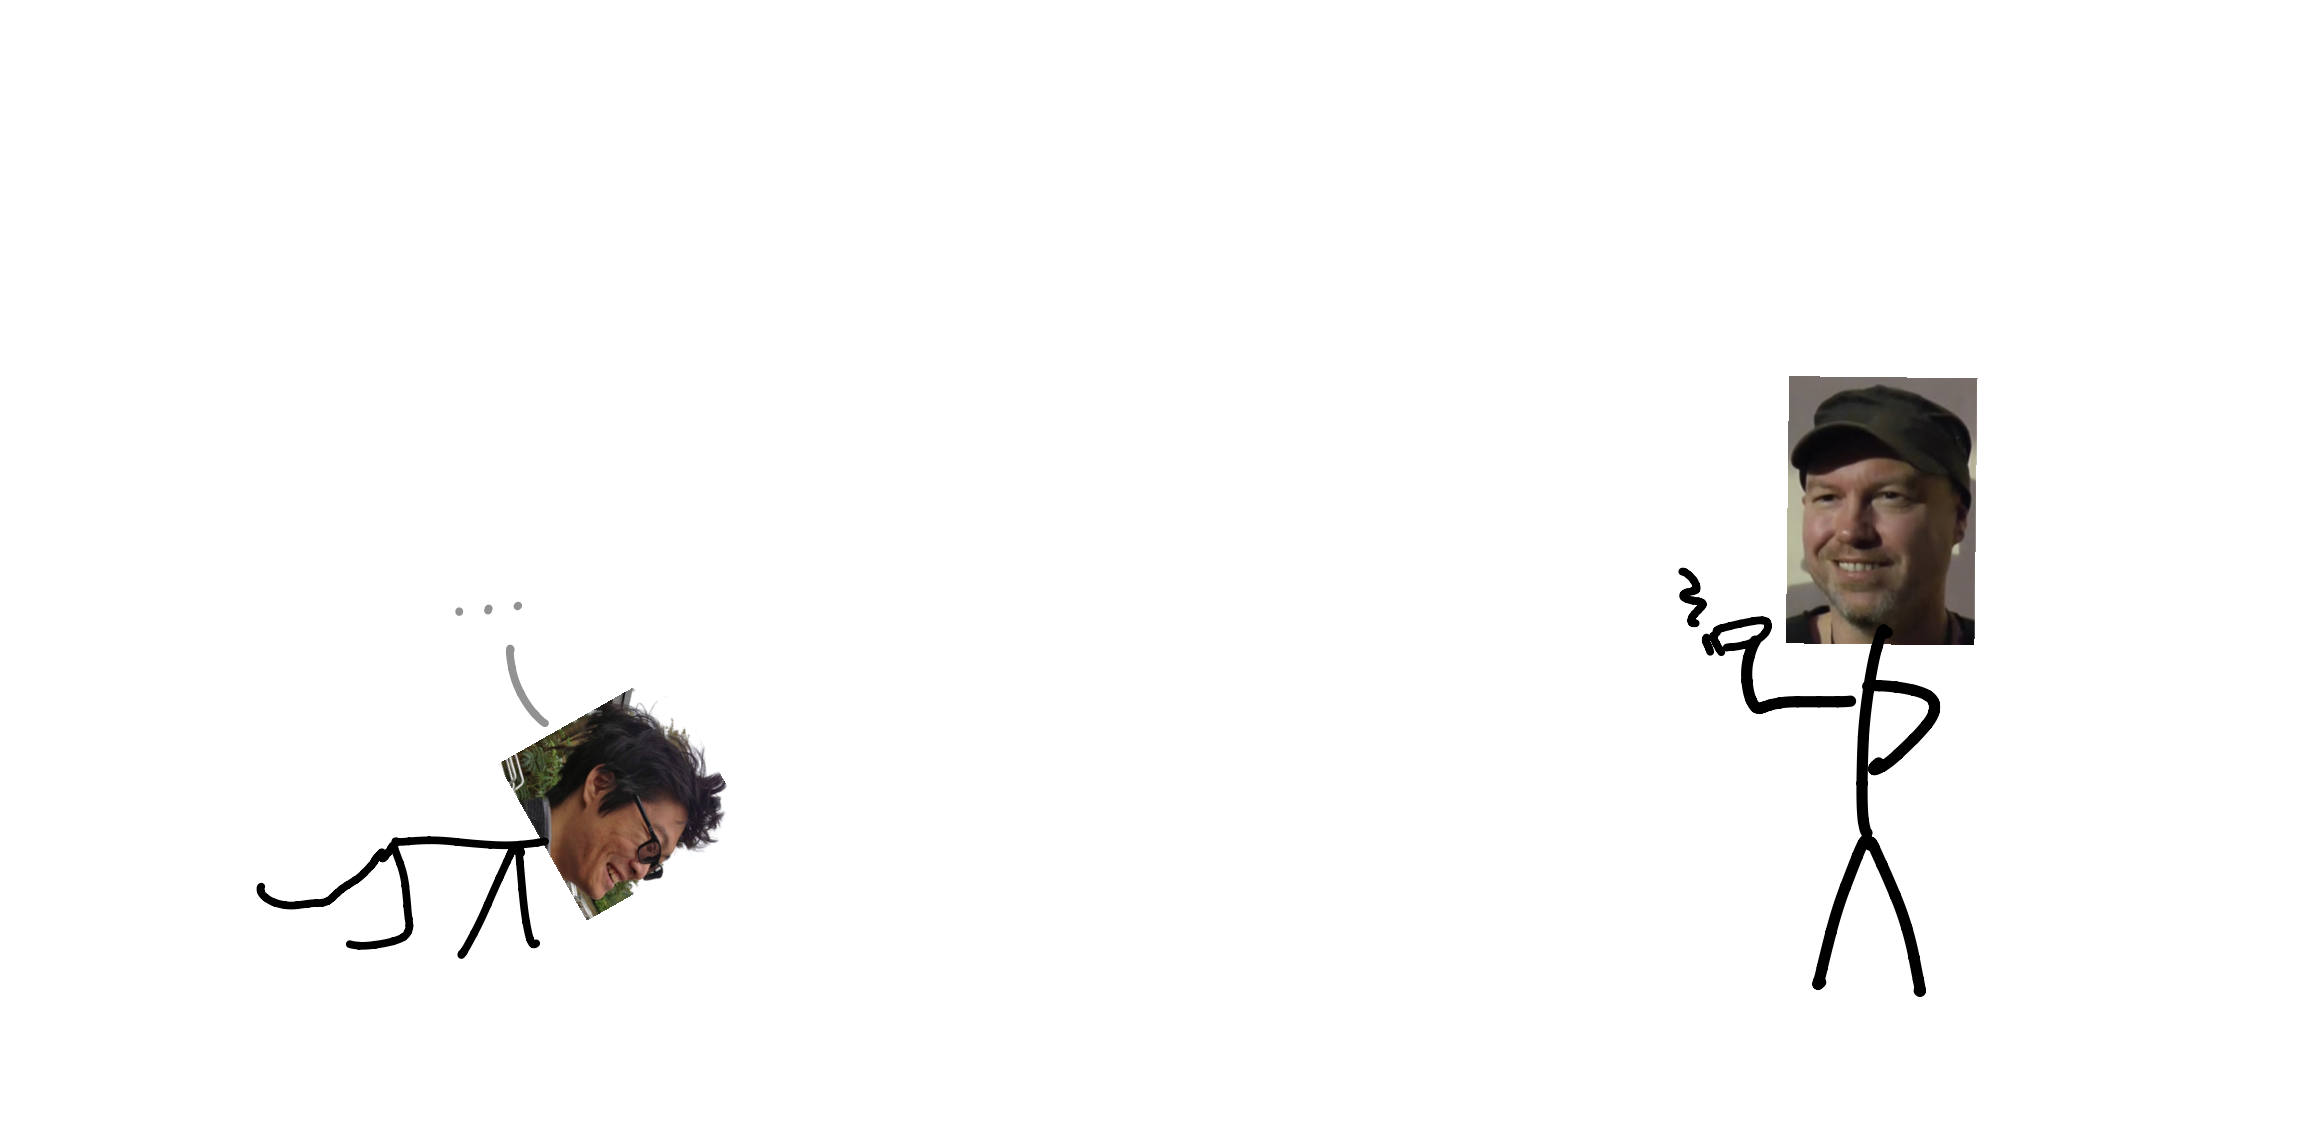
\includegraphics{figures/cartoons/pregroup4}}
\caption{Bob had a good point. Everything worked, but we had no understanding as to why, and accordingly, whether or not it would all break. At this point in time, Jonathon Liu, a masters' student I tutored during COVID, had committed the grave error of thinking diagrams were cool, and was now hanging out with me and Bob. After understanding the procedure, Jono independently devised the same arcane internal wirings as I had, but neither of us could explain how we did it. So we had evidence of an underlying governing structure that was coherent but inarticulable.}
\end{figure}

\begin{figure}[h!]
\centering
\scalebox{1}{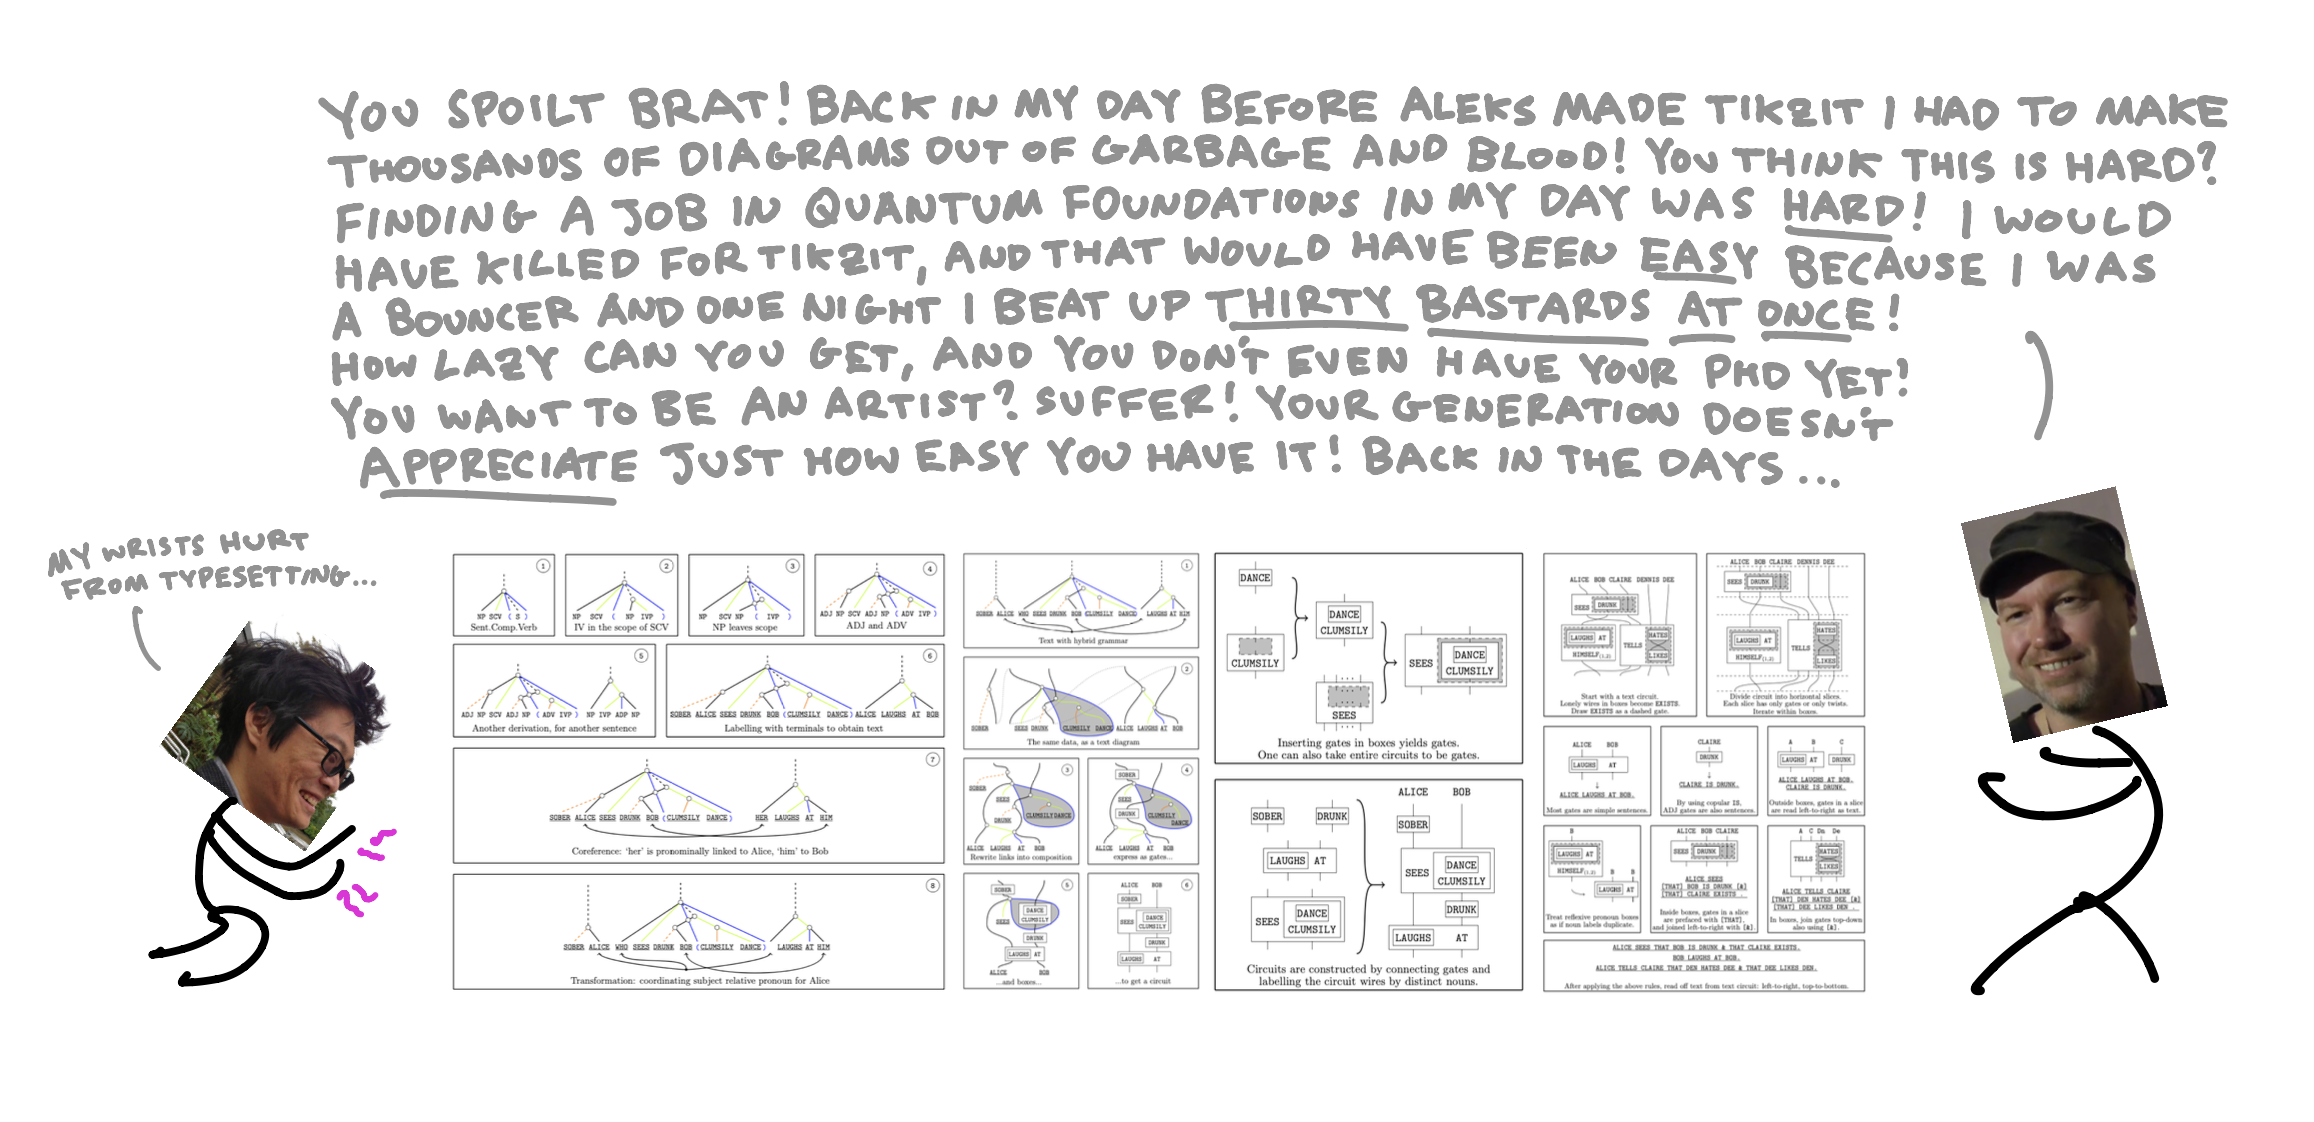
\includegraphics{figures/cartoons/bigpaper1}}
\caption{I realised that our intuitions were coming from an implicit productive grammar, rather than a parsing one, and that the path of least resistance for obtaining formal guarantees for the language-to-circuit procedure was to just handcraft a generative grammar for the fragment of language we were interested in. This meant scrapping everything in the first draft and starting again from scratch. Bob always had a word of gentle encouragement, giving me the motivation to persevere.\\

So now we had two ways to obtain text circuits. One from pregroups (which Jono had extended the technique for to CCGs in his master's thesis \bR CITE \e), and one from handcrafted productive grammars. Then came time for me to write my thesis, and there were three salient questions I wanted to address.\\
Firstly, what are internal wirings?\\
Secondly, how do text circuits relate to other generative grammars?\\
Thirdly, what are text circuits good for?\\
These questions are now what the rest of the thesis seeks to answer.
}
\end{figure}



\bibliographystyle{alpha}
\bibliography{thesis_intro}





\end{document}